%-------------------------------------------------------------------------------
%	PACKAGES AND OTHER DOCUMENT CONFIGURATIONS
%-------------------------------------------------------------------------------

\documentclass[
11pt, % The default document font size, options: 10pt, 11pt, 12pt
%oneside, % Two side (alternating margins) for binding by default, uncomment to switch to one side
english, % ngerman for German
singlespacing, % Single line spacing, alternatives: onehalfspacing or doublespacing
%draft, % Uncomment to enable draft mode (no pictures, no links, overfull hboxes
%indicated) nolistspacing, % If the document is onehalfspacing or doublespacing,
%uncomment this to set spacing in lists to single liststotoc, % Uncomment to add
%the list of figures/tables/etc to the table of contents toctotoc, % Uncomment
%to add the main table of contents to the table of contents parskip, % Uncomment
%to add space between paragraphs nohyperref, % Uncomment to not load the
%hyperref package
headsepline, % Uncomment to get a line under the header
%chapterinoneline, % Uncomment to place the chapter title next to the number on one line
%consistentlayout, % Uncomment to change the layout of the declaration, abstract and acknowledgements pages to match the default layout
]{MastersThesis} % The class file specifying the document structure

\usepackage[utf8]{inputenc} % Required for inputting international characters
\usepackage[T1]{fontenc} % Output font encoding for international characters

\usepackage{mathpazo} % Use the Palatino font by default
\usepackage{tikz}
\usepackage{acronym} % Acronyms
\usetikzlibrary{decorations.pathreplacing,positioning, arrows.meta}
\newcommand{\ImageWidth}{11cm}
\definecolor{myLightGray}{RGB}{191,191,191}
\definecolor{myGray}{RGB}{160,160,160}
\definecolor{myDarkGray}{RGB}{144,144,144}
\definecolor{myDarkRed}{RGB}{167,114,115}
\definecolor{myRed}{RGB}{255,58,70}
\definecolor{myGreen}{RGB}{0,255,71}
\usepackage{hyperref}
\usepackage{parskip}
\usepackage{algorithm}
\usepackage{algpseudocode}
\usepackage{etoolbox}
\usepackage{enumitem}
\usepackage[most]{tcolorbox}
\usepackage{siunitx}
\DeclareSIUnit{\voltpeak}{Vp}
\usepackage{svg}
\usepackage{tikz-3dplot}
\usepackage[a]{esvect}
\usepackage{lipsum}
\usepackage{amsthm}
\usepackage{etoolbox} % for patching
\tcbuselibrary{theorems}


% REFs/Citations/Acronyms/Links blue

% Define boxed definition environment with no rounded corners
\tcolorboxenvironment{definition}{
  enhanced,
  colback=red!5,            % light red background
  boxrule=0pt,            % border thickness
  arc=0mm,                  % no rounded corners
  sharp corners,            % enforce sharp edges
  top=0mm,
  bottom=1mm,
  left=2mm,
  right=2mm,
  before skip=10pt,
  after skip=10pt
}
\tcolorboxenvironment{theorem}{
  enhanced,
  colback=gray!10,        % light grey background
  boxrule=0pt,            % no border
  arc=0mm,
  sharp corners,
  top=0mm,
  bottom=1mm,
  left=2mm,
  right=2mm,
  before skip=10pt,
  after skip=10pt
}

\theoremstyle{definition}
\newtheorem{definition}{Definition}[section]
\theoremstyle{plain}
\newtheorem{theorem}[definition]{Theorem}
\makeatletter
\patchcmd{\@begintheorem}{\ignorespaces}{\vspace{1em}\ignorespaces}{}{}
\patchcmd{\@opargbegintheorem}{\ignorespaces}{\vspace{1em}\ignorespaces}{}{}
\patchcmd{\@endtheorem}{\unskip}{\unskip\vspace{1em}}{}{}
\makeatother

\theoremstyle{remark}
\newtheorem{remark}{Remark}[section]
\theoremstyle{remark}
\newtheorem{example}{Example}[section]

\usetikzlibrary{decorations.pathmorphing} % for zigzag


% Linecomments in algorithms
\usepackage{xcolor}
\newcommand{\commentsymbol}{\textcolor{green!50!black}{//}}% or \% or $\triangleright$
\algrenewcommand\algorithmiccomment[1]{\hfill {\color{green!50!black}\commentsymbol{} #1}}
\makeatletter
\newcommand{\LineComment}[2][\algorithmicindent]{\Statex \hspace{#1}{\color{green!50!black}\commentsymbol{} #2}}
\makeatother
\newcommand{\varfont}{\texttt}

% \usepackage{cleveref}

% \hypersetup{
%     colorlinks=true,
%     linkcolor=blue,
%     filecolor=magenta,      
%     urlcolor=cyan,
%     pdftitle={Overleaf Example},
%     pdfpagemode=FullScreen,
% }

\usepackage[backend=bibtex,natbib=true]{biblatex} % Use the bibtex backend with the authoryear citation style (which resembles APA)

\addbibresource{example.bib} % The filename of the bibliography

\usepackage[autostyle=true]{csquotes} % Required to generate language-dependent quotes in the bibliography

%----------------------------------------------------------------------------------------
%	MARGIN SETTINGS
%----------------------------------------------------------------------------------------

\geometry{
	paper=a4paper, % Change to letterpaper for US letter
	inner=2.5cm, % Inner margin
	outer=3.8cm, % Outer margin
	bindingoffset=.5cm, % Binding offset
	top=1.5cm, % Top margin
	bottom=1.5cm, % Bottom margin
	head=27.2pt, % Adjust head height to avoid warnings
	%showframe, % Uncomment to show how the type block is set on the page
}

%----------------------------------------------------------------------------------------
%	THESIS INFORMATION
%----------------------------------------------------------------------------------------

\thesistitle{Quasi-Monte Carlo Methods and Applications} % Your thesis title, this is used in the title and abstract, print it elsewhere with \ttitle
\supervisor{Prof. Dr. Andreas \textsc{Neuenkirch}} % Your supervisor's name, this is used in the title page, print it elsewhere with \supname
\examiner{} % Your examiner's name, this is not currently used anywhere in the template, print it elsewhere with \examname
\degree{Master of Science} % Your degree name, this is used in the title page and abstract, print it elsewhere with \degreename
\author{Janik V. \textsc{Hrubant}} % Your name, this is used in the title page and abstract, print it elsewhere with \authorname
\addresses{} % Your address, this is not currently used anywhere in the template, print it elsewhere with \addressname

\subject{Mathematics} % Your subject area, this is not currently used anywhere in the template, print it elsewhere with \subjectname
\keywords{} % Keywords for your thesis, this is not currently used anywhere in the template, print it elsewhere with \keywordnames
\university{\href{https://www.uni-mannheim.de/en/}{University of Mannheim}} % Your university's name and URL, this is used in the title page and abstract, print it elsewhere with \univname
\department{\href{http://department.university.com}{Department or School Name}} % Your department's name and URL, this is used in the title page and abstract, print it elsewhere with \deptname
\group{\href{http://researchgroup.university.com}{Research Group Name}} % Your research group's name and URL, this is used in the title page, print it elsewhere with \groupname
\faculty{\href{http://faculty.university.com}{Faculty Name}} % Your faculty's name and URL, this is used in the title page and abstract, print it elsewhere with \facname

\AtBeginDocument{
\hypersetup{pdftitle=\ttitle} % Set the PDF's title to your title
\hypersetup{pdfauthor=\authorname} % Set the PDF's author to your name
\hypersetup{pdfkeywords=\keywordnames} % Set the PDF's keywords to your keywords
}

\begin{document}

\frontmatter % Use roman page numbering style (i, ii, iii, iv...) for the pre-content pages

\pagestyle{plain} % Default to the plain heading style until the thesis style is called for the body content

%----------------------------------------------------------------------------------------
%	TITLE PAGE
%----------------------------------------------------------------------------------------

\begin{titlepage}
\begin{center}

\vspace*{.06\textheight}
{\scshape\LARGE \univname\par}\vspace{1.5cm} % University name
\textsc{\Large Master Thesis}\\[0.5cm] % Thesis type

\HRule \\[0.4cm] % Horizontal line
{\huge \bfseries \ttitle\par}\vspace{0.4cm} % Thesis title
\HRule \\[1.5cm] % Horizontal line
 
\begin{minipage}[t]{0.4\textwidth}
\begin{flushleft} \large
\emph{Author:}\\
\authorname % Author name - remove the \href bracket to remove the link
\end{flushleft}
\end{minipage}
\begin{minipage}[t]{0.4\textwidth}
\begin{flushright} \large
\emph{Supervisors:} \\
\supname % Supervisor name - remove the \href bracket to remove the link  
\end{flushright}
\end{minipage}\\[3cm]
 
\vfill

\large \textit{A thesis submitted in fulfillment of the requirements\\ for the degree of \degreename}\\[0.3cm] % University requirement text
\textit{in the}\\[0.4cm]
\groupname\\\deptname\\[2cm] % Research group name and department name
 
\vfill

{\large \today}\\[4cm] % Date
%\includegraphics{Logo} % University/department logo - uncomment to place it
 
\vfill
\end{center}
\end{titlepage}

%----------------------------------------------------------------------------------------
%	DECLARATION PAGE
%----------------------------------------------------------------------------------------

\begin{declaration}
\addchaptertocentry{\authorshipname} % Add the declaration to the table of contents
Hiermit versichere ich, dass diese Arbeit von mir persönlich verfasst wurde und
dass ich keinerlei fremde Hilfe in Anspruch genommen habe. Ebenso versichere
ich, dass diese Arbeit oder Teile daraus weder von mir selbst noch von anderen
als Leistungsnachweise andernorts eingereicht wurden. Wörtliche oder sinngemäße
Übernahmen aus anderen Schriften und Veröffentlichungen in gedruckter oder
elektronischer Form sind ge- kennzeichnet. Sämtliche Sekundärliteratur und
sonstige Quellen sind nachgewiesen und in der Bibliographie aufgeführt. Das
Gleiche gilt für graphische Darstellungen und Bilder sowie für alle
Internet-Quellen. Ich bin ferner damit einverstanden, dass meine Arbeit zum
Zwecke eines Plagiatsabgleichs in elektronischer Form anonymisiert versendet und
gespeichert werden kann. Mir ist bekannt, dass von der Korrektur der Arbeit ab-
gesehen werden kann, wenn diese Erklärung nicht erteilt wird.
 
\noindent Signed:\\
\rule[0.5em]{25em}{0.5pt} % This prints a line for the signature
 
\noindent Date:\\
\rule[0.5em]{25em}{0.5pt} % This prints a line to write the date
\end{declaration}

\cleardoublepage

%-------------------------------------------------------------------------------
%	QUOTATION PAGE
%-------------------------------------------------------------------------------

% \vspace*{0.2\textheight}

% \noindent\enquote{\itshape Thanks to my solid academic training, today I can write hundreds of words on virtually any topic without possessing a shred of information, which is how I got a good job in journalism.}\bigbreak

% \hfill Dave Barry

%-------------------------------------------------------------------------------
%	ABSTRACT PAGE
%-------------------------------------------------------------------------------d

\begin{abstract}
\addchaptertocentry{\abstractname} % Add the abstract to the table of contents
\lipsum[1-2]
% The idea of PRP is to help both, stores and distribuition centers by making arguable suggestions to automize their replenishment decisions. As their replenishment decisions highly impact their service and different retailers like Mirgros, Coop, Aldi or Lidl have cardinaly different strategies, these tools need to be adjusted for customer needs and product requirements. these results are highly dependent on Notably boths business results are highly dependent from their replanishment decisions on either restocking stores from deliveries by distribuition centers or distribuition center from further suppliers. \\
% These decisions are arguably taken to the \emph{Theory of Constraints (TOC)}
% Procurement of goods and products is a multifaceted process that presents substantial challenges for companies. Each decision, notably those around supplier orders, requires a comprehensive understanding of numerous essential business factors and limitations.This process begins with the critical task of demand prediction, followed by assessing variable prices relative to order quantities and optimizing logistics considering the spatial and weight capacities of transport methods. Concurrently, while striving to maintain ample inventory, companies must be cognizant of definite expiration dates and anticipate potential spoilage.\\
% This thesis concentrates on the accumulation of research outcomes pertaining to multiple dimensions and strategies for resolving the intricate optimization problem inherent in replenishment planning.\\
% Funded by SAP, this research project is aimed at providing informed recommendations to the development team to enhance production code, ultimately leading to the creation of the Predictive Replenishment Planning (PRP) tool, a feature within the S4/HANA Cloud offering.
\end{abstract}

%-------------------------------------------------------------------------------
%	ACKNOWLEDGEMENTS
%-------------------------------------------------------------------------------

% \begin{acknowledgements}
% \addchaptertocentry{\acknowledgementname} % Add the acknowledgements to the table of contents
% The acknowledgments and the people to thank go here, don't forget to include your project advisor\ldots
% \end{acknowledgements}

%-------------------------------------------------------------------------------
%	LIST OF CONTENTS/FIGURES/TABLES PAGES
%-------------------------------------------------------------------------------

\tableofcontents % Prints the main table of contents

% \listoffigures % Prints the list of figures

% \listoftables % Prints the list of tables

%-------------------------------------------------------------------------------
%	ABBREVIATIONS
%-------------------------------------------------------------------------------

\newpage
\begin{acronym}
\acro{rita}[RITA]{Rational Inverse Transform with Aliasing}
\acro{cdf}[CDF]{Cumulative Distribution Function}
\acro{qmc}[QMC]{Quasi-Monte Carlo}
\acro{mc}[MC]{Monte Carlo}
\acro{hu}[HU]{Hounsfield Unit}
\acro{ct}[CT]{Computed Tomography}
\acro{cbct}[CBCT]{Cone-Beam Computed Tomography}
\acro{ffd}[FFD]{Forced Fixed Detection}
\acro{cnn}[CNN]{Convolutional Neural Network}
\acro{dnn}[DNN]{Deep Neural Network}
\acro{pde}[PDE]{Partial Differential Equation}
\end{acronym}

%-------------------------------------------------------------------------------
%	PHYSICAL CONSTANTS/OTHER DEFINITIONS
%-------------------------------------------------------------------------------

% \begin{constants}{lr@{${}={}$}l} % The list of physical constants is a three column table

% % The \SI{}{} command is provided by the siunitx package, see its documentation for instructions on how to use it

% Speed of Light & $c_{0}$ & \SI{2.99792458e8}{\meter\per\second} (exact)\\
% %Constant Name & $Symbol$ & $Constant Value$ with units\\

% \end{constants}

%-------------------------------------------------------------------------------
%	SYMBOLS
%-------------------------------------------------------------------------------

% \begin{symbols}{lll} % Include a list of Symbols (a three column table)

% $a$ & distance & \si{\meter} \\
% $P$ & power & \si{\watt} (\si{\joule\per\second}) \\
% %Symbol & Name & Unit \\

% \addlinespace % Gap to separate the Roman symbols from the Greek

% $\omega$ & angular frequency & \si{\radian} \\

% \end{symbols}

%-------------------------------------------------------------------------------
%	ACRONYMS
%-------------------------------------------------------------------------------

\acro{rita}[RITA]{Rational Inverse Transform with Aliasing}
\acro{cdf}[CDF]{Cumulative Distribution Function}
\acro{qmc}[QMC]{Quasi-Monte Carlo}
\acro{mc}[MC]{Monte Carlo}
\acro{hu}[HU]{Hounsfield Unit}
\acro{ct}[CT]{Computed Tomography}
\acro{cbct}[CBCT]{Cone-Beam Computed Tomography}
\acro{ffd}[FFD]{Forced Fixed Detection}
\acro{cnn}[CNN]{Convolutional Neural Network}
\acro{dnn}[DNN]{Deep Neural Network}
\acro{pde}[PDE]{Partial Differential Equation}

%-------------------------------------------------------------------------------
%	DEDICATION
%-------------------------------------------------------------------------------

% \dedicatory{For/Dedicated to/To my\ldots} 

%-------------------------------------------------------------------------------
%	THESIS CONTENT - CHAPTERS
%-------------------------------------------------------------------------------

\mainmatter % Begin numeric (1,2,3...) page numbering

\pagestyle{thesis} % Return the page headers back to the "thesis" style

% Include the chapters of the thesis as separate files from the Chapters folder
% Uncomment the lines as you write the chapters

%!TEX root = ../main.tex
\part{Fundamentals of Quasi-Monte Carlo Methods}
\label{part1}

\chapter{Monte Carlo and Quasi-Monte Carlo Integration}
\label{chapter1}

% ------------------------------------------------------------------------------
% ------------------------------------------------------------------------------
\section{Motivation and Problem Setting}
% ------------------------------------------------------------------------------
% ------------------------------------------------------------------------------
The numerical evaluation of high-dimensional integrals is a fundamental task in
modern applied mathematics and scientific computing. Applications range from
Bayesian inference and financial mathematics to machine learning and
computational physics. In particular, contemporary domains such as deep neural
network training and medical imaging often require the estimation of integrals
of the form

\begin{equation}
    \label{eq:integration_problem}
    I(f) = \int_{[0,1]^s} f(x)\,dx\,,
\end{equation}

where $s$ denotes the dimensionality of the problem and $f$ is a function that
may be expensive or impractical to evaluate analytically.

One of the most widely used approaches to compute such integrals is the
classical \ac{mc} method, which estimates the expectation based on averages over
randomly sampled points. The primary appeal of \ac{mc} integration lies in its
dimension-independent convergence rate and minimal assumptions on the integrand.
However, its asymptotic error rate of $\mathcal{O}(N^{-1/2})$ limits its
efficiency -- especially when high precision is required or function evaluations
are computationally expensive.

\ac{qmc} methods offer an alternative paradigm: instead of random samples, they employ deterministic sequences -- so-called low-discrepancy sequences—that aim to fill the integration domain more uniformly. This structured sampling allows for faster convergence under certain smoothness conditions and forms the basis for many state-of-the-art techniques in high-dimensional numerical integration.

The goal of this part is to develop a rigorous mathematical foundation for
\ac{qmc} methods and to understand how they improve upon classical Monte Carlo
integration. The key concepts introduced here -- particularly discrepancy theory
and low-discrepancy sequences -- serve as theoretical tools that will be
revisited in later parts of this thesis.
Chapter~\ref{chapter2} will delve into the
measurement of uniformity via star discrepancy and provide concrete
constructions of low-discrepancy sequences such as Sobol and Halton, which are
central to the numerical methods applied in Part~\ref{part2} and
Part~\ref{part3}, dedicated to neural network training and CT-based photon
transport simulation.


% ------------------------------------------------------------------------------
\subsection{High-Dimensional Integration in Applications}
% ------------------------------------------------------------------------------
High-dimensional integration problems arise naturally in a wide range of
scientific and engineering disciplines. Whenever expectations with respect to
multivariate distributions must be computed numerically, they are typically
formulated as integrals over the $s$-dimensional unit cube -- such as the
integral in Equation~\eqref{eq:integration_problem}.

Prominent examples include:
\begin{itemize}
    \item \textbf{Bayesian statistics}: Computing posterior expectations, marginal likelihoods, or predictive distributions.
    \item \textbf{Financial mathematics}: Pricing complex financial derivatives and evaluating risk measures under stochastic models.
    \item \textbf{Machine learning}: Estimating expectations in variational inference, training neural networks using randomized optimization techniques, or evaluating generalization bounds.
    \item \textbf{Medical imaging}: Simulating photon transport and estimating physical quantities based on noisy measurements, especially in \ac{ct} and magnetic resonance imaging (MRI).
\end{itemize}

In all these cases, the dimensionality $s$ can be moderate to very high --
sometimes even exceeding hundreds or thousands of variables. This introduces
significant challenges for numerical integration methods, which must balance
accuracy, computational cost, and robustness with respect to the structure of
the integrand.

The remainder of this chapter explores how \ac{mc} and \ac{qmc} methods address
these challenges. Before doing so, we briefly review the Monte Carlo method and
its fundamental convergence properties in the next section.


% ------------------------------------------------------------------------------
\subsection{Monte Carlo Integration: Principle and Convergence}
% ------------------------------------------------------------------------------
The classical \ac{mc} method is a probabilistic approach to numerical
integration that relies on random sampling. It is particularly suited for
high-dimensional settings, as its convergence rate does not deteriorate with
increasing dimension.

\begin{definition}[Monte Carlo Estimator] \ \\
Let $f \in L^2([0,1]^s)$ and let $X_0, \dots, X_{N-1} \sim
\mathcal{U}([0,1]^s)$ be independent and identically distributed random samples.
The Monte Carlo estimator of the integral \( I \) is given by
\begin{equation}
    I_N^{\mathrm{MC}}(f) := \frac{1}{N} \sum_{n=0}^{N-1} f(X_n)\,.
\end{equation}
\end{definition}


This estimator is unbiased and converges almost surely to the true integral as $N \to \infty$, as established by the Strong Law of Large Numbers:

\begin{theorem}[Strong Law of Large Numbers] \ \\
Let $f \in L^2([0,1]^s)$. Then
\begin{equation}
\mathbb{P}\left[ \lim_{N \to \infty} I_N^{\mathrm{MC}}(f) = \int_{[0,1]^s} f(x)\, dx \right] = 1.
\end{equation}
\end{theorem}

Beyond this almost sure convergence, the expected integration error of the Monte
Carlo estimator can be quantified using the root-mean-square error \cite[Section 1.3]{pillichshammer2010zahlentheoretische}:

\begin{theorem}[Monte Carlo Convergence Rate] \ \\
\label{thm:mc-convergence-rate}
Let $f \in L^2([0,1]^s)$. Then
\begin{equation}
    \mathbb{E}\left[ \left| I_N^{\mathrm{MC}}(f) - I(f) \right| \right] \leq \frac{\sigma[f]}{\sqrt{N}},
\end{equation}
where $\sigma[f] := \sqrt{\mathrm{Var}[f]}$.
\end{theorem}

\begin{proof}[Sketch of Proof]
Using independence and linearity of expectation, the variance of $I_N^{\mathrm{MC}}(f)$ is
\begin{equation}
    \mathrm{Var}[I_N^{\mathrm{MC}}(f)] = \frac{\mathrm{Var}[f]}{N}.
\end{equation}
Applying Jensen's inequality yields the stated bound on the expected absolute error.
\end{proof}

\begin{remark}
The convergence rate $\mathcal{O}(N^{-1/2})$ is independent of the integration
dimension $s$, which is a key advantage of the Monte Carlo method. In contrast,
classical grid-based methods often suffer from the curse of dimensionality,
where the number of required samples grows exponentially with $s$.
\end{remark}

\begin{example}
Let $f \in C^1([0,1]^s)$ be a Lipschitz-continuous function. A uniform grid with
$N = m^s$ points has a worst-case error of $\mathcal{O}(N^{-1/s})$. In high
dimensions, this becomes prohibitively inefficient, while MC integration retains
the dimension-agnostic rate $\mathcal{O}(N^{-1/2})$. \cite[Section
1.1]{leobacher2014introduction}
\end{example}

Despite its robustness and simplicity, MC integration has several well-known limitations:
\begin{itemize}
    \item The convergence rate is relatively slow, especially for smooth integrands.
    \item Error bounds are probabilistic rather than deterministic.
    \item The method does not exploit structural properties of the integrand, such as smoothness or sparsity.
\end{itemize}

These limitations motivate the development of quasi-Monte Carlo methods, which
will be introduced in the next section.


% ------------------------------------------------------------------------------
% ------------------------------------------------------------------------------
\section{Quasi-Monte Carlo Methods}
% ------------------------------------------------------------------------------
% ------------------------------------------------------------------------------

% ------------------------------------------------------------------------------
\subsection{Deterministic Sampling and Intuition}
% ------------------------------------------------------------------------------

Classical \ac{mc} methods approximate integrals over the unit cube $[0,1]^s$
using randomly sampled points. In contrast, \ac{qmc} methods replace
stochasticity with a deterministic strategy, aiming to cover the integration
domain in a more uniform and structured way.

\begin{definition}[Quasi-Monte Carlo Estimator] \ \\
Let $f \colon [0,1]^s \to \mathbb{R}$ be a measurable function and let
$\{\boldsymbol{x}_n\}_{n=1}^{N} \subset [0,1]^s$ be a deterministic point set.
Then the \emph{quasi-Monte Carlo estimator} for the integral
\begin{equation*}
    I(f) = \int_{[0,1]^s} f(\boldsymbol{x}) \, d\boldsymbol{x}
\end{equation*}
is defined as
\begin{equation}
I_N^{\mathrm{QMC}}(f) := \frac{1}{N} \sum_{n=1}^{N} f(\boldsymbol{x}_n).
\end{equation}
\end{definition}

The functions $I$, $I_N^{\mathrm{MC}}$ and $I_N^{\mathrm{QMC}}$ will be further
used without explicit reference to the integrand $f$ when the context is clear.

Unlike in the Monte Carlo setting, these points are not drawn from a probability
distribution, but are generated deterministically — typically by rules that aim
to avoid clustering and oversampling.

Figure~\ref{fig:mc-vs-qmc} illustrates this contrast by comparing $300$ randomly
sampled points to $300$ \ac{qmc} points from the Sobol' sequence in two
dimensions. The quasi-Monte Carlo points distribute more evenly, avoiding both
gaps and clusters.

\begin{figure}[H]
  \centering
  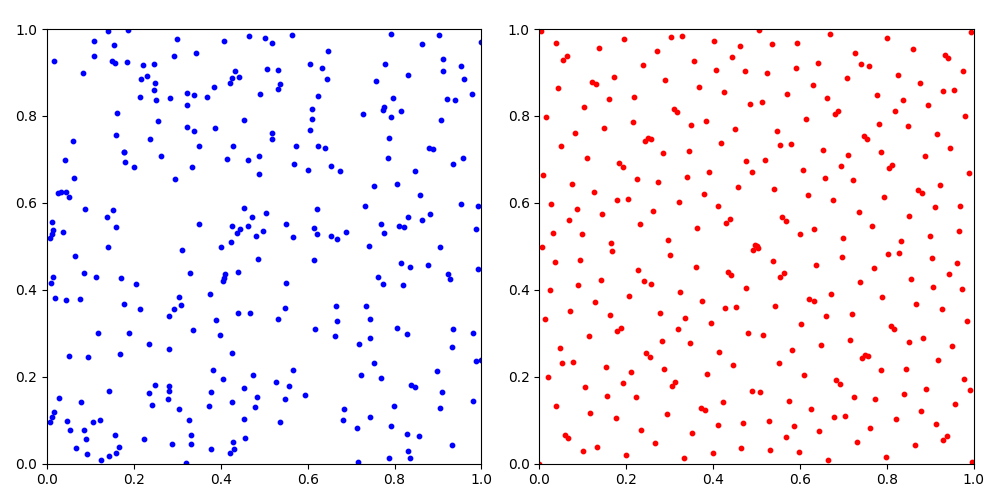
\includegraphics[width=0.8\textwidth]{Figures/mc_vs_qmc.png}
  \caption{Comparison of $300$ sample points in $[0,1]^2$ using (left) standard 
  Monte Carlo and (right) a Sobol' sequence. \ac{qmc} points avoid clustering and 
  fill the domain more evenly.}
  \label{fig:mc-vs-qmc}
\end{figure}

A natural alternative to \ac{mc} sampling is the use of regular tensor-product
grids. However, these grids suffer from the \emph{curse of dimensionality}:
placing $m$ points per dimension leads to a total of $N = m^s$ points, which
becomes infeasible even for moderate $s$. Furthermore, grids are not easily
extensible -- adding new points requires global recomputation and destroys
nesting.

By contrast, many \ac{qmc} sequences, such as Sobol' and Halton (will be
introduced in Chapter~\ref{chapter2}), are designed to be \emph{incremental}:
each new point can be added without changing the existing ones. This makes
\ac{qmc} particularly suitable for adaptive algorithms, especially for anytime
algorithms that might increment the number of samples needed over time. However,
not all \ac{qmc} constructions share this feature such as lattice rules and some
optimized designs are fixed-size by nature.

\ac{qmc} methods thus offer the best of both worlds: they combine the
space-filling structure of grids with the flexibility and scalability of
sampling methods. Low-discrepancy sequences fill the space more evenly than
random points while avoiding the redundancy of regular grids. This often leads
to significantly lower integration errors, especially for smooth functions or
problems with low effective dimension.

This shift from probabilistic to deterministic sampling also changes the way we
analyze error: instead of using statistical bounds, we rely on \emph{discrepancy
measures}, which quantify the uniformity of the point set. These concepts, along
with the notion of function variation, will be introduced in the following
sections.

\begin{remark}
\ac{qmc} estimators retain the same algebraic structure as their \ac{mc}
counterparts, but their convergence behavior is governed by entirely different
theoretical tools -- namely discrepancy theory and function variation.
\end{remark}


% ------------------------------------------------------------------------------
\subsection{Monte Carlo vs. Quasi-Monte Carlo: A First Comparison}
\label{subsec:mc-vs-qmc}
% ------------------------------------------------------------------------------

\ac{mc} and \ac{qmc} methods share the same high-level goal: estimating an
integral by averaging function evaluations at selected sample points. The
difference lies in the sampling strategy -- stochastic versus deterministic --
and the consequences this has for accuracy, convergence and theoretical
guarantees.

Table~\ref{tab:mc-vs-qmc} summarizes key conceptual distinctions between the two paradigms.

\begin{table}[H]
\centering
\resizebox{0.95\textwidth}{!}{
\renewcommand{\arraystretch}{1.4}
\begin{tabular}{l|c|c}
\textbf{Aspect} & \textbf{Monte Carlo (MC)} & \textbf{Quasi-Monte Carlo (QMC)} \\
\hline
Sampling & Independent random points & Deterministic low-discrepancy points \\
Error bounds & Probabilistic (in expectation) & Deterministic (worst-case) \\
Regularity assumptions on $f$ & Square integrability ($L^2$) & Bounded variation (HK) \\
Theoretical convergence & $\mathcal{O}(N^{-1/2})$ & Up to $\mathcal{O}(N^{-1})$ (heuristic) \\
Point extensibility & Trivial & Often supported (e.g., Sobol) \\
Robustness to noise & High & Low \\
\end{tabular}}
\caption{Conceptual comparison of Monte Carlo and quasi-Monte Carlo integration methods.}
\label{tab:mc-vs-qmc}
\end{table}

While \ac{mc} estimators are unbiased and robust even under minimal assumptions,
their convergence is slow and does not improve when the integrand is smooth.
\ac{qmc} methods, on the other hand, exploit structure in the integrand -- such
as smoothness or low effective dimension -- and can yield significantly lower
integration errors.

However, \ac{qmc} methods lack probabilistic guarantees and depend more strongly
on the careful construction of the point set. Their performance can degrade if
the integrand exhibits high variability along many input dimensions or if the
chosen sequence is not well matched to the function.

The next subsection discusses the convergence rates of both methods in more
detail and highlights the interplay between dimensionality and integration
error.


% ------------------------------------------------------------------------------
\subsection{Convergence Rates and the Curse of Dimensionality}
\label{subsec:convergence-vs-dimension}
% ------------------------------------------------------------------------------

A major appeal of the Monte Carlo method is its dimension-agnostic convergence
behavior from Theorem~\ref{thm:mc-convergence-rate}. Under the assumption that
$f \in L^2([0,1]^s)$, the root-mean-square error of the MC estimator satisfies

\begin{equation}
    \mathbb{E}[ | I_N^{\mathrm{MC}} - I |] = \mathcal{O}(N^{-1/2}),
\end{equation}

regardless of the dimension $s$. This makes \ac{mc} a go-to method for very
high-dimensional problems, even when no structure in the integrand is known or
exploitable.

\ac{qmc} methods, while lacking this universality, offer a fundamentally
different convergence profile. For sufficiently regular integrands
(specifically, those of bounded variation in the sense of Hardy and Krause), the
integration error of \ac{qmc} estimators is bounded by

\begin{equation}
    | I_N^{\mathrm{QMC}} - I | \leq D_N^* \cdot V_{\mathrm{HK}}(f),
\end{equation}

where $D_N^*$ is the star discrepancy of the point set and $V_{\mathrm{HK}}(f)$
is the Hardy--Krause variation of the integrand (both formalized later in
\textcolor{blue}{\textbf{TODO}}). For well-constructed low-discrepancy
sequences, it is known that

\begin{equation}
    D_N^* = \mathcal{O}\left( \frac{(\log N)^s}{N} \right).
\end{equation}

This bound implies a near-linear convergence rate in $N$ -- much faster than
\ac{mc} -- but introduces a logarithmic dependence on the dimension $s$. As $s$
increases, the factor $(\log N)^s$ grows rapidly, leading to the curse of
dimensionality in worst-case \ac{qmc} analysis.

Fortunately, in many practical problems, the \emph{effective dimension} of the
integrand is much lower than its nominal input dimension. That is, most of the
function's variation is concentrated along a small number of directions. When
this is the case, QMC methods frequently outperform MC in practice, even in
problems with moderately high $s$.

\begin{example}
In deep learning applications, such as training neural networks, stochastic
gradients often lie near low-dimensional manifolds. Similarly, in CT-based
simulation models, the system's physical response depends more strongly on a few
dominant input parameters. These scenarios are highly favorable for QMC.
\end{example}

We will revisit the precise meaning of discrepancy and variation -- and how they
control the QMC error -- in Chapters~\ref{chapter2} and \ref{chapter3}.


% ------------------------------------------------------------------------------
\section{Uniformity Concepts}
\label{sec:uniformity-concepts}
% ------------------------------------------------------------------------------

The efficiency of \ac{qmc} methods hinges on how well the employed point sets
"fill" the integration domain $[0,1]^s$. This motivates the need for a precise
mathematical understanding of \emph{uniformity}. The present section introduces
two key concepts in this regard -- \emph{uniform distribution modulo one} and
\emph{equidistribution} -- and clarifies their relevance to numerical
integration.

% ------------------------------------------------------------------------------
\subsection{Uniform Distribution vs. Equidistribution}
% ------------------------------------------------------------------------------

While the terms \emph{uniform distribution} and \emph{equidistribution} are
sometimes used interchangeably in informal contexts, they carry distinct
meanings in the context of numerical integration. In quasi-Monte Carlo methods,
the notion of \emph{uniform distribution modulo one} provides a rigorous
criterion for how evenly a sequence covers the unit cube. This concept forms the
foundation for analyzing the convergence behavior of QMC estimators.

\begin{definition}[Uniform Distribution Modulo One] \ \\
Let $(\boldsymbol{x}_n)_{n \in \mathbb{N}_0} \subset [0,1]^s$ be a sequence of
sample points. The sequence is said to be \emph{uniformly distributed modulo
one} (u.d.\ mod~1) if, for every axis-aligned box $[\boldsymbol{a},
\boldsymbol{b}) \subset [0,1]^s$, the proportion of points falling into this box
converges to its Lebesgue measure:
\begin{equation*}
    \lim_{N \to \infty} \frac{1}{N} \sum_{n=0}^{N-1} \chi_{[\boldsymbol{a}, \boldsymbol{b})}(\boldsymbol{x}_n)
    = \lambda_s([\boldsymbol{a}, \boldsymbol{b})) \,,
\end{equation*}
where $\lambda_s$ denotes the $s$-dimensional Lebesgue measure and $\chi_A$ is
the indicator function of the set $A$.
\end{definition}

This definition emphasizes asymptotic spatial coverage: in the limit, every
subregion of the domain is sampled proportionally to its volume. Importantly,
this property is purely deterministic and does not rely on any probabilistic
assumptions — in contrast to Monte Carlo methods, which only guarantee
uniformity in expectation.

In contrast, when speaking of a random sample $\{X_1, \dots, X_N\} \subset [0,1]^s$ drawn i.i.d.\ from the uniform distribution, we refer to a probabilistic concept of uniformity: each point is independently drawn according to the uniform measure, but the empirical distribution may not be uniformly spread in finite samples. Thus, equidistribution refers to the ideal uniform coverage that we seek deterministically, while uniform random sampling only ensures this behavior in expectation or with high probability.

\begin{remark}
Uniform distribution modulo one is a necessary condition for the convergence of quasi-Monte Carlo estimators. If a point sequence is not u.d.\ mod 1, then there exists at least one Riemann-integrable function for which the sample average fails to converge to the integral.
\end{remark}

The following result, known as Weyl’s criterion, provides a necessary and sufficient condition for uniform distribution in terms of exponential sums.

\begin{theorem}[Weyl's Criterion] \ \\
A sequence $(\boldsymbol{x}_n)_{n \geq 0} \subset [0,1)^s$ is uniformly distributed modulo one if and only if, for all nonzero $\boldsymbol{h} \in \mathbb{Z}^s \setminus \{\boldsymbol{0}\}$, we have
\begin{equation*}
    \lim_{N \to \infty} \frac{1}{N} \sum_{n=0}^{N-1} \exp(2\pi i\, \boldsymbol{h} \cdot \boldsymbol{x}_n) = 0.
\end{equation*}
\end{theorem}

\begin{example}
Let $\alpha \in \mathbb{R}$ be irrational. Then the Kronecker sequence $(n \alpha \bmod 1)_{n \geq 0}$ is uniformly distributed in $[0,1]$. This is a consequence of Weyl’s criterion and illustrates the existence of simple, deterministic sequences with excellent uniformity properties.
\end{example}

% ------------------------------------------------------------------------------
\subsection{Why Uniformity Matters in Numerical Integration}
% ------------------------------------------------------------------------------

In \ac{qmc} integration, the objective is to approximate the integral defined in
Equation~\eqref{eq:integration_problem} by a finite average over a deterministic
point set $\{\boldsymbol{x}_0, \dots, \boldsymbol{x}_{N-1}\} \subset [0,1]^s$.
The accuracy of this approximation depends crucially on how uniformly the point
set samples the domain.

Unlike \ac{mc} methods, which rely on probabilistic guarantees and
variance-based error estimates, \ac{qmc} methods exploit deterministic
structure: the integration error is directly influenced by how well the point
set fills the domain. This insight gives rise to one of the most fundamental
theoretical tools in \ac{qmc} analysis: the \emph{Koksma--Hlawka inequality}.

\begin{remark}
The Koksma--Hlawka inequality bounds the integration error of a QMC estimator by
the product of two quantities: the \emph{star discrepancy} of the point set and
the \emph{variation} of the integrand in the sense of Hardy and Krause. In
short,
\begin{equation*}
    \left| \frac{1}{N} \sum_{n=0}^{N-1} f(\boldsymbol{x}_n) - I \right| 
    \leq D_N^*(\{\boldsymbol{x}_n\}) \cdot V_{\mathrm{HK}}(f).
\end{equation*}
A rigorous statement and detailed discussion of this inequality will follow in
Chapter~\ref{chapter3}.
\end{remark}

This inequality highlights why uniformity is essential: if the integrand has
bounded variation, then smaller discrepancy directly implies smaller integration
error. In this sense, discrepancy theory becomes a cornerstone of effective
\ac{qmc} integration.

\begin{remark}
The star discrepancy quantifies the maximal deviation between the empirical
distribution of the point set and the uniform distribution over $[0,1]^s$. It
vanishes asymptotically for uniformly distributed sequences and governs the
convergence behavior of \ac{qmc} estimators.
\end{remark}

The next chapter provides a formal introduction to discrepancy theory. We will
define extreme and star discrepancy, study their geometric interpretation, and
analyze the behavior of structured low-discrepancy sequences such as Halton and
Sobol'. These sequences, due to their uniform space-filling properties, play a
central role in modern high-dimensional numerical integration.

\chapter{Discrepancy Theory and Low-Discrepancy Sequences}
\label{chapter2}

% ------------------------------------------------------------------------------
\section{Measuring Uniformity: Discrepancy}
% ------------------------------------------------------------------------------

One of the cornerstones of \ac{qmc} theory is the concept of \emph{discrepancy},
which quantifies how uniformly a finite point set samples the $s$-dimensional
unit cube $[0,1]^s$. While uniform distribution modulo one describes the
asymptotic behavior of infinite sequences, discrepancy provides a finite-sample
measure of deviation from perfect uniformity. Low-discrepancy sequences are the
foundation of \ac{qmc} methods because they minimize this deviation and thus
yield more accurate numerical integration.

This section introduces formal definitions, geometric intuition and empirical
insights into discrepancy measures. It lays the theoretical groundwork for
understanding how the structure of point sets affects \ac{qmc} integration
performance.

% ------------------------------------------------------------------------------
\subsection{Definition of Discrepancy and Star Discrepancy}
% ------------------------------------------------------------------------------

First, we define the more general \emph{extreme discrepancy}:

\begin{definition}[Extreme Discrepancy] \ \\
Let $\mathcal{P}\subset [0,1)^s$, with $|\mathcal{P}| = N$, being a finite point
set. Then the extreme discrepancy $D_N(\mathcal{P})$ is defined as
\begin{equation*}
    D_N(\mathcal{P}) = \sup\limits_{\substack{\boldsymbol{a,b} \in [0,1]^s \\ \boldsymbol{a} \leq \boldsymbol{b}}} \bigg| \frac{A([\boldsymbol{a},\boldsymbol{b}) , \mathcal{P}, N)}{N} - \lambda_s([\boldsymbol{a},\boldsymbol{b})] \bigg|.
\end{equation*}
Hereby $A([\boldsymbol{a},\boldsymbol{b}), \mathcal{P}, N)$ denotes the number
of points in $\mathcal{P}$ that fall into the box
$[\boldsymbol{a},\boldsymbol{b})$, and
$\lambda_s([\boldsymbol{a},\boldsymbol{b})]$ is the Lebesgue measure of that
box, given by $\prod_{i=1}^{s} (b_i - a_i)$.
\end{definition}

In practice, a common and slightly more tractable variant is the \emph{star
discrepancy}, which restricts the test boxes to be anchored at the origin.

\begin{definition}[Star Discrepancy] \ \\
Let $\mathcal{P}\subset [0,1)^s$, with $|\mathcal{P}| = N$, being a finite point
set. Then the star discrepancy $D_N^*$ is defined as
\begin{equation*}
    D_N^*(\mathcal{P}) = \sup\limits_{\boldsymbol{t} \in [0,1]^s} \bigg| \frac{A([\boldsymbol{0},\boldsymbol{t}), \mathcal{P}, N)}{N} - \lambda_s([\boldsymbol{0},\boldsymbol{t})] \bigg|.
\end{equation*}
\end{definition}

This form is used in the Koksma--Hlawka inequality and serves as a central
measure in \ac{qmc} analysis. Note that both discrepancy definitions are
deterministic and depend solely on the point configuration.

\begin{remark}
A low star discrepancy implies that the empirical distribution of the points
approximates the uniform distribution well over all axis-aligned subrectangles
anchored at the origin.
\end{remark}

% ------------------------------------------------------------------------------
\subsection{Geometric Interpretation and Examples}
% ------------------------------------------------------------------------------

To build geometric intuition, consider the 1-dimensional case. Given $N$ sample
points $x_0, \dots, x_{N-1} \in [0,1)$, we can visualize discrepancy as the
maximum vertical deviation between the empirical distribution function
\begin{equation*}
F_N(t) := \frac{1}{N} \sum_{n=0}^{N-1} \chi_{[0,t)}(x_n)
\end{equation*}
and the uniform cumulative distribution function $F(t) = t$. The discrepancy
corresponds to the largest gap between $F_N(t)$ and $F(t)$.

In higher dimensions, the idea generalizes: the star discrepancy measures the
maximal difference in the number of points falling into an axis-aligned box
$[\boldsymbol{0}, \boldsymbol{t})$ versus the volume of that box. Intuitively,
it quantifies whether the point set "overpopulates" or "underpopulates" certain
regions.

\begin{figure}[H]
\centering
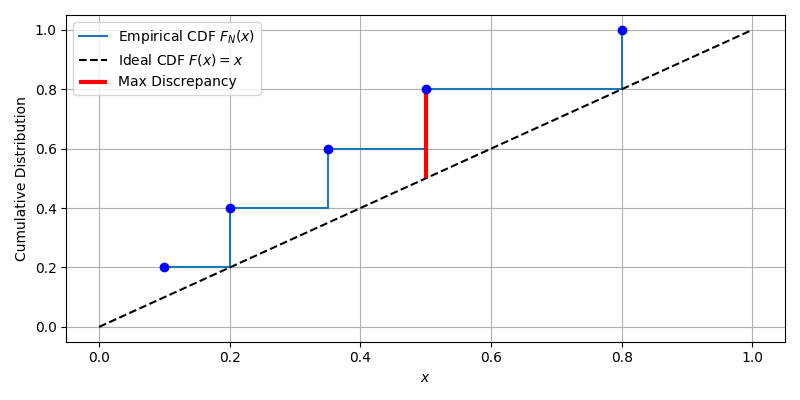
\includegraphics[scale=.67]{Figures/discrepancy1d.png}
\caption{Visualization of 1D discrepancy: the maximum vertical distance between the empirical CDF $F_N(t)$ and the uniform CDF $F(t) = t$.}
\label{fig:discrepancy-1d}
\end{figure}

\begin{example}
Let $x_n = \frac{n}{N}$ for $n = 0, \dots, N-1$. Then $F_N(t)$ is a
piecewise constant staircase function, and the discrepancy can be shown to be
$\mathcal{O}(1/N)$. This is an optimal rate in 1D.
\end{example}

\begin{remark}
Discrepancy provides a worst-case error metric over all subintervals. Thus, even
a point set that appears visually well-distributed may have large discrepancy
due to subtle gaps or clustering in certain regions.
\end{remark}

% ------------------------------------------------------------------------------
\subsection{Empirical Observation of Discrepancy in QMC}
% ------------------------------------------------------------------------------

Discrepancy is not just a theoretical construct -- its practical relevance
becomes evident when comparing the behavior of \ac{qmc} sequences with \ac{mc}
samples. In particular, structured point sets like Halton and Sobol sequences
achieve much lower discrepancy than random samples of the same size.

\begin{figure}[H]
\centering
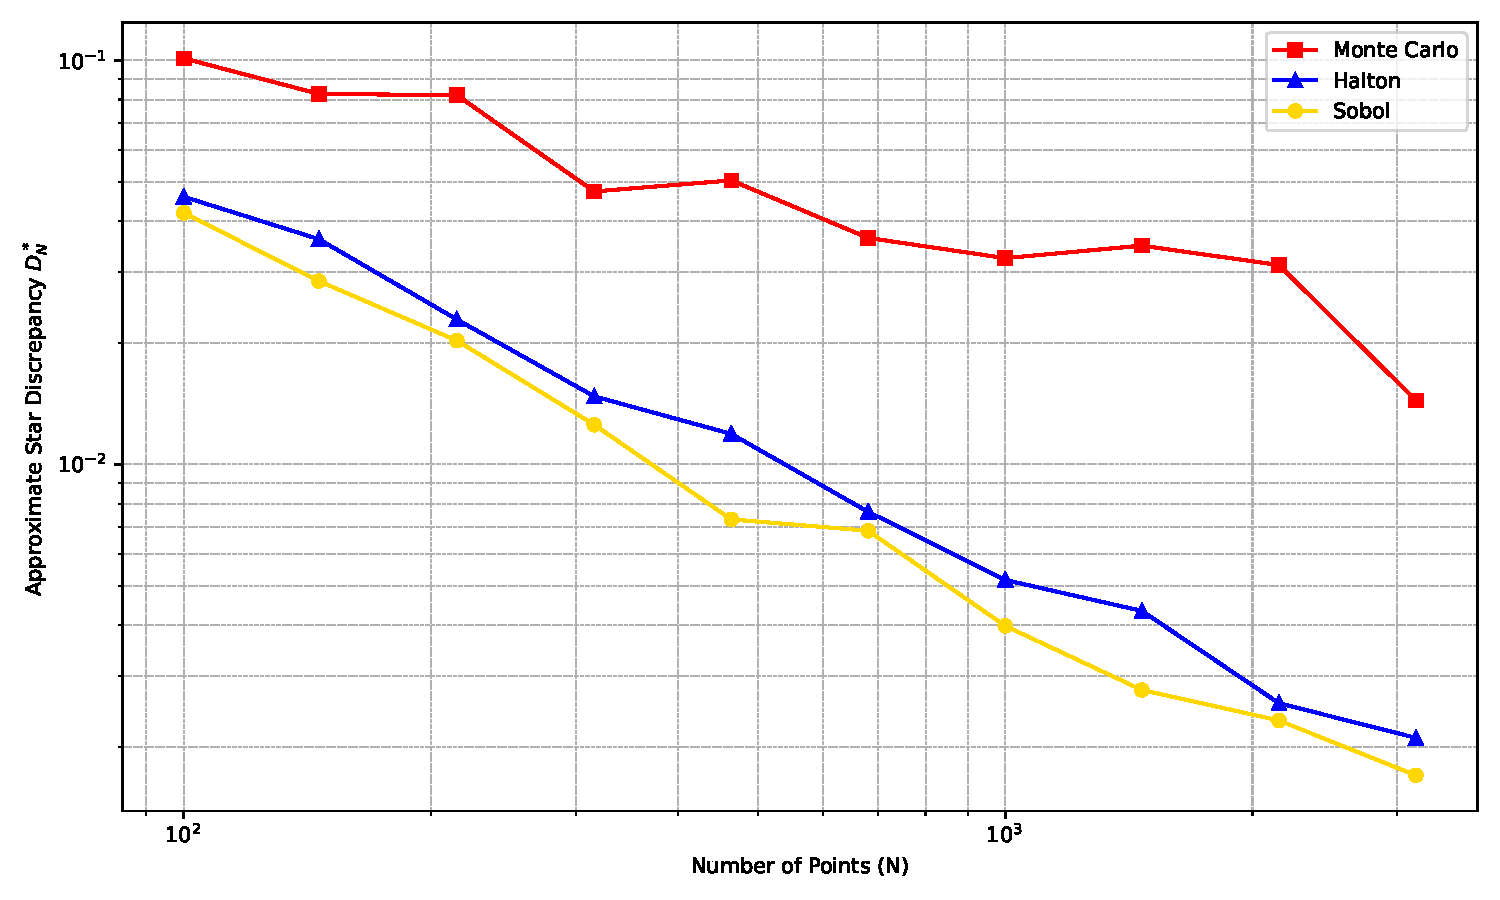
\includegraphics[width=0.9\textwidth]{Figures/qmc_discrepancy_comparison.pdf}
\caption{Comparison of discrepancy growth for Sobol, Halton and random (\ac{mc})
point sets in 2D. Low-discrepancy sequences exhibit significantly slower
discrepancy growth.}
\label{fig:qmc-discrepancy-comparison}
\end{figure}

\begin{remark}
The expected star discrepancy of i.i.d. Monte Carlo samples decreases at the
rate $\mathcal{O}(N^{-1/2})$, whereas for low-discrepancy sequences, provable
upper bounds of order $\mathcal{O}((\log N)^s / N)$ exist.
\cite[Section~2.2]{leobacher2014introduction}
\end{remark}

The next section will introduce specific constructions of low-discrepancy
sequences and analyze their dimensional performance and implementation details.


% ------------------------------------------------------------------------------
\section{Construction of Low-Discrepancy Sequences}
% ------------------------------------------------------------------------------
In this section, we will explore several well-known constructions of
low-discrepancy sequences, focusing on their mathematical foundations and
properties.


% ------------------------------------------------------------------------------
\subsection{The Halton Sequence}
\label{subsec:halton-sequence}
% ------------------------------------------------------------------------------

The Halton sequence is one of the earliest and most widely used constructions of low-discrepancy sequences in arbitrary dimensions. It generalizes the one-dimensional van der Corput sequence to multiple dimensions by using mutually prime bases.

\begin{definition}[Halton Sequence]
Let $b_1, \dots, b_s$ be pairwise coprime integers greater than $1$, typically
chosen as the first $s$ prime numbers. The $n$-th point $\boldsymbol{x}_n \in
[0,1)^s$ of the $s$-dimensional Halton sequence is defined componentwise by
\begin{equation*}
    \boldsymbol{x}_n = \left( \phi_{b_1}(n), \dots, \phi_{b_s}(n) \right),
\end{equation*}
where $\phi_b(n)$ denotes the van der Corput radical-inverse function in base
$b$. The Halton sequence is then given by $\mathcal{S}_{b_1, \dots, b_s} = (x_n)_{n\in \mathbb{N}}$.
\end{definition}

\begin{example}[First Elements of the Halton Sequence in 2D] \ \\
Consider the two-dimensional Halton sequence based on the first two prime bases $b_1 = 2$ and $b_2 = 3$. The first three elements are obtained by computing the radical-inverse values $\phi_{b_1}(n)$ and $\phi_{b_2}(n)$ for $n = 1, 2, 3$:

\begin{itemize}
    \item $n = 1$: $\boldsymbol{x}_1 = \left( \phi_2(1), \phi_3(1) \right) = \left( \tfrac{1}{2}, \tfrac{1}{3} \right)$
    \item $n = 2$: $\boldsymbol{x}_2 = \left( \phi_2(2), \phi_3(2) \right) = \left( \tfrac{1}{4}, \tfrac{2}{3} \right)$
    \item $n = 3$: $\boldsymbol{x}_3 = \left( \phi_2(3), \phi_3(3) \right) = \left( \tfrac{3}{4}, \tfrac{1}{9} \right)$
\end{itemize}

This illustrates how the Halton sequence fills the unit square in a low-discrepancy manner even for small $n$.
\end{example}






The radical-inverse function $\phi_b(n)$ maps an integer $n$ to a real number in $[0,1)$ by reflecting its base-$b$ representation about the decimal point:
\begin{equation*}
    \phi_b(n) = \sum_{k=0}^\infty d_k b^{-k-1}, \quad \text{where } n = \sum_{k=0}^\infty d_k b^k.
\end{equation*}

Intuitively, this construction ensures that each component of the sequence explores the unit interval in a structured, non-redundant way. By combining several one-dimensional van der Corput sequences in different coprime bases, the resulting multi-dimensional point set avoids regular grid-like patterns and achieves asymptotic uniformity.

The Halton sequence has star discrepancy of order
\begin{equation*}
    D_N^*(\{\boldsymbol{x}_0, \dots, \boldsymbol{x}_{N-1}\}) = \mathcal{O}\left( \frac{(\log N)^s}{N} \right),
\end{equation*}
making it a prototypical example of a low-discrepancy sequence. However, for
larger dimensions, correlation effects between the different base components can
lead to degraded uniformity and higher discrepancy. Variants such as scrambling
or leaping are commonly employed to mitigate this issue.

\begin{remark}
The Halton sequence is extensible in $N$ and $s$, making it suitable for
applications that require growing or adaptive point sets. However, its
performance in high dimensions is often inferior to more modern constructions
like the Sobol sequence.
\end{remark}


% ------------------------------------------------------------------------------
  \subsection{The Sobol Sequence}
% ------------------------------------------------------------------------------



% ------------------------------------------------------------------------------
    \subsubsection{Direction Numbers and Gray Code}
% ------------------------------------------------------------------------------



% ------------------------------------------------------------------------------
    \subsubsection{Scrambling Techniques for Sobol}
% ------------------------------------------------------------------------------



% ------------------------------------------------------------------------------
  \subsection{Dimensional Performance and Sequence Comparison}
% ------------------------------------------------------------------------------

\part{Quasi-Monte Carlo Sampling for Neural Network Training}

\chapter{Motivation and Problem Formulation}

\begin{itemize}
    \item Many-query problems and the need for surrogate models
    \item Limitations of randomly sampled training data in DNNs
    \item Formal definition of the supervised learning setup
    \item Motivation for using low-discrepancy sampling in training
\end{itemize}

% % Chapter Template

% \chapter{Neural Network Training with QMC in Deterministic Settings} % Main chapter title

% \label{Chapter3} % Change X to a consecutive number; for referencing this chapter elsewhere, use \ref{ChapterX}

% %----------------------------------------------------------------------------------------
% %	SECTION 1
% %----------------------------------------------------------------------------------------

% \section{Problem Setup and Input Space Design}

% Lorem ipsum dolor sit amet, consectetur adipiscing elit. Aliquam ultricies lacinia euismod. Nam tempus risus in dolor rhoncus in interdum enim tincidunt. Donec vel nunc neque. In condimentum ullamcorper quam non consequat. Fusce sagittis tempor feugiat. Fusce magna erat, molestie eu convallis ut, tempus sed arcu. Quisque molestie, ante a tincidunt ullamcorper, sapien enim dignissim lacus, in semper nibh erat lobortis purus. Integer dapibus ligula ac risus convallis pellentesque.

% %----------------------------------------------------------------------------------------
% %	SECTION 2
% %----------------------------------------------------------------------------------------

% \section{Generation of Training Sets via QMC and MC}

% Sed ullamcorper quam eu nisl interdum at interdum enim egestas. Aliquam placerat justo sed lectus lobortis ut porta nisl porttitor. Vestibulum mi dolor, lacinia molestie gravida at, tempus vitae ligula. Donec eget quam sapien, in viverra eros. Donec pellentesque justo a massa fringilla non vestibulum metus vestibulum. Vestibulum in orci quis felis tempor lacinia. Vivamus ornare ultrices facilisis. Ut hendrerit volutpat vulputate. Morbi condimentum venenatis augue, id porta ipsum vulputate in. Curabitur luctus tempus justo. Vestibulum risus lectus, adipiscing nec condimentum quis, condimentum nec nisl. Aliquam dictum sagittis velit sed iaculis. Morbi tristique augue sit amet nulla pulvinar id facilisis ligula mollis. Nam elit libero, tincidunt ut aliquam at, molestie in quam. Aenean rhoncus vehicula hendrerit.

% %----------------------------------------------------------------------------------------
% %	SECTION 3
% %----------------------------------------------------------------------------------------

% \section{Network Architecture and Training Protocols}

% Sed ullamcorper quam eu nisl interdum at interdum enim egestas. Aliquam placerat justo sed lectus lobortis ut porta nisl porttitor. Vestibulum mi dolor, lacinia molestie gravida at, tempus vitae ligula. Donec eget quam sapien, in viverra eros. Donec pellentesque justo a massa fringilla non vestibulum metus vestibulum. Vestibulum in orci quis felis tempor lacinia. Vivamus ornare ultrices facilisis. Ut hendrerit volutpat vulputate. Morbi condimentum venenatis augue, id porta ipsum vulputate in. Curabitur luctus tempus justo. Vestibulum risus lectus, adipiscing nec condimentum quis, condimentum nec nisl. Aliquam dictum sagittis velit sed iaculis. Morbi tristique augue sit amet nulla pulvinar id facilisis ligula mollis. Nam elit libero, tincidunt ut aliquam at, molestie in quam. Aenean rhoncus vehicula hendrerit.

% %----------------------------------------------------------------------------------------
% %	SECTION 4
% %----------------------------------------------------------------------------------------

% \section{Convergence Evaluation and Error Metrics}

% Sed ullamcorper quam eu nisl interdum at interdum enim egestas. Aliquam placerat justo sed lectus lobortis ut porta nisl porttitor. Vestibulum mi dolor, lacinia molestie gravida at, tempus vitae ligula. Donec eget quam sapien, in viverra eros. Donec pellentesque justo a massa fringilla non vestibulum metus vestibulum. Vestibulum in orci quis felis tempor lacinia. Vivamus ornare ultrices facilisis. Ut hendrerit volutpat vulputate. Morbi condimentum venenatis augue, id porta ipsum vulputate in. Curabitur luctus tempus justo. Vestibulum risus lectus, adipiscing nec condimentum quis, condimentum nec nisl. Aliquam dictum sagittis velit sed iaculis. Morbi tristique augue sit amet nulla pulvinar id facilisis ligula mollis. Nam elit libero, tincidunt ut aliquam at, molestie in quam. Aenean rhoncus vehicula hendrerit.

% %----------------------------------------------------------------------------------------
% %	SECTION 5
% %----------------------------------------------------------------------------------------

% \section{Comparative Results}

% Sed ullamcorper quam eu nisl interdum at interdum enim egestas. Aliquam placerat justo sed lectus lobortis ut porta nisl porttitor. Vestibulum mi dolor, lacinia molestie gravida at, tempus vitae ligula. Donec eget quam sapien, in viverra eros. Donec pellentesque justo a massa fringilla non vestibulum metus vestibulum. Vestibulum in orci quis felis tempor lacinia. Vivamus ornare ultrices facilisis. Ut hendrerit volutpat vulputate. Morbi condimentum venenatis augue, id porta ipsum vulputate in. Curabitur luctus tempus justo. Vestibulum risus lectus, adipiscing nec condimentum quis, condimentum nec nisl. Aliquam dictum sagittis velit sed iaculis. Morbi tristique augue sit amet nulla pulvinar id facilisis ligula mollis. Nam elit libero, tincidunt ut aliquam at, molestie in quam. Aenean rhoncus vehicula hendrerit.
%!TEX root = ../main.tex
\part{Quasi-Monte Carlo Sampling for Neural Network Training}
\label{part2}

\chapter{Motivation and Problem Formulation}
\label{chapter4}

The second part of this thesis investigates the application of \acfp{qmc}
sampling techniques to enhance the training of \acfp{dnn} in \emph{many-query
problems} -- computational tasks in which a parameterized map must be evaluated for
a large number of inputs, each requiring costly simulations or numerical
solutions of PDEs. This situation arises frequently in scientific computing,
e.g. in uncertainty quantification, Bayesian inversion, optimal control and
model calibration.

Such problems motivate the use of surrogate models $\hat{f}_\theta$, typically
based on deep neural networks, which are trained offline on a set of inputs and
then used for fast evaluation online. However, using random sampling for
generating training data yields to star discrepancy $\mathcal{O}(N^{-1/2})$ as
introduced in Part~\ref{part1}.

To overcome this limitation, this thesis explores the use of low-discrepancy sequences as training data which fill the input domain more
uniformly. Under mild regularity assumptions, they can significantly reduce the
generalization error due to improved equidistribution properties.

\section{Many-Query Problems in Scientific Computing}
Many-query problems refer to scenarios in which a computationally expensive
model $f(x)$ must be evaluated for many different parameter values $x \in
\mathcal{X} \subset \mathbb{R}^s$. Typical applications include:
\begin{itemize}
  \item \textbf{Uncertainty quantification (UQ)}: Compute statistics of $f(x)$
  for uncertain $x$.
  \item \textbf{Optimal design/control}: Evaluate objective functions $f(x)$ for
  many designs $x$.
  \item \textbf{Inverse problems}: Repeatedly evaluate $f(x)$ during parameter
  inference.
\end{itemize}

The sheer cost of evaluating $f(x)$ (e.g., via numerical PDE solvers) motivates
the use of surrogate models. Once trained, a surrogate $\hat{f}_\theta$ can
provide rapid predictions for unseen inputs at a fraction of the computational
cost.

\section{The Role of Function Approximation}
We formalize the problem as learning a map $f \colon [0,1]^s \to \mathbb{R}^m$
from data. The assumption of a unit hypercube domain reflects common practice in
\ac{qmc} theory and is justified via homeomorphic mappings from more general
compact and simply connected input spaces.

The surrogate model $\hat{f}_\theta$ can be chosen from the class of deep neural
networks and trained on data $\{(x_i, f(x_i))\}_{i=1}^N$. The aim is to
approximate $f$ with high accuracy while minimizing the number of required
evaluations.

\aclp{dnn} are known to be universal approximators. Under mild conditions on the
later introduced \emph{activation functions} they proved to be able to
approximate any continuous function on compact sets arbitrarily well
\cite{cybenko1989approximation}.

\section{Limitations of Random Sampling in Neural Network Training}
Typically, training data is generated using \acl{mc} sampling, where points $x_i$ are drawn independently and identically distributed (i.i.d.) according to a probability measure $\mu$ on $[0,1]^s$. Under this approach, statistical learning theory provides an estimate for the expected generalization error $\mathbb{E}[E_G]$ as follows:
\begin{equation*}
\mathbb{E}[E_G] \leq E_T + \mathcal{O}\left(\frac{1}{\sqrt{N}}\right),
\end{equation*}
where $E_T$ is the empirical training error. However, as argued
in~\cite{mishra2021enhancing}, this rate is unsatisfactory in many-query
problems because:
\begin{itemize}
  \item A small generalization error requires a large $N$, which is costly due
  to expensive evaluations of $f(x)$.
  \item The constant in the bound depends on the variance and correlations in
  the training process, which are hard to control.
\end{itemize}

\section{QMC-Based Surrogates: A Promising Alternative}
Low-discrepancy sequences (Sobol', Halton, etc.) provide a way to sample the
domain $[0,1]^s$ more uniformly than random sampling. In \acl{qmc} theory, the Koksma-Hlawka inequality (Theorem~\ref{thm:koksma-hlawka}) gives an error bound of the form
\begin{equation*}
|E_G - E_T| \leq V_{\mathrm{HK}}(|f - \hat{f}_\theta|) \cdot D^*_N \leq  V_{\mathrm{HK}}(|f - \hat{f}_\theta|) \cdot C \frac{(\log N)^s}{N},
\end{equation*}
where $V_{\mathrm{HK}}$ denotes the Hardy--Krause variation and $D^*_N$ is the
star-discrepancy of the training points.

This suggests that \ac{qmc} sampling can lead to significantly smaller generalization
gaps -- especially when $f$ has bounded variation and the activation functions used
in $\hat{f}_\theta$ are smooth.

\section{Overview of Part~\ref{part2}} The remainder of this part is structured
as follows:
\begin{itemize}
  \item \textbf{Chapter~\ref{chapter5}} introduces the mathematical foundations
  of deep neural networks and their use in function approximation.
  \item \textbf{Chapter~\ref{chapter6}} discusses the concepts of training and
  generalization error, including classical and QMC-based bounds.
  \item \textbf{Chapter~\ref{chapter7}} presents the theoretical analysis of
  QMC-based training, including discrepancy, variation, and convergence
  guarantees.
  \item \textbf{Chapter~\ref{chapter8}} provides an empirical evaluation
  comparing QMC and Monte Carlo training strategies across different benchmark
  tasks.
\end{itemize}

The ultimate goal of this part is to demonstrate that quasi-random sampling
provides a viable and theoretically grounded strategy to reduce the cost and
improve the accuracy of deep neural network training in scientific computing.


%!TEX root = ../main.tex
\chapter{Theoretical Foundations of QMC-Based Learning}

\begin{itemize}
    \item Adapting QMC theory to supervised learning
    \item Hardy-Krause variation of the loss function
    \item Generalization error bounds using low-discrepancy samplin\item 
    \item Comparison to MC-based bounds and practical implication\item 
    \item Validity conditions and smoothness assumptions
\end{itemize}

% % Chapter Template

% \chapter{Neural Network Training for Stochastic Functions} % Main chapter title

% \label{Chapter4} % Change X to a consecutive number; for referencing this chapter elsewhere, use \ref{ChapterX}

% %----------------------------------------------------------------------------------------
% %	SECTION 1
% %----------------------------------------------------------------------------------------

% \section{Modeling Randomness in Physical Simulations}

% Lorem ipsum dolor sit amet, consectetur adipiscing elit. Aliquam ultricies lacinia euismod. Nam tempus risus in dolor rhoncus in interdum enim tincidunt. Donec vel nunc neque. In condimentum ullamcorper quam non consequat. Fusce sagittis tempor feugiat. Fusce magna erat, molestie eu convallis ut, tempus sed arcu. Quisque molestie, ante a tincidunt ullamcorper, sapien enim dignissim lacus, in semper nibh erat lobortis purus. Integer dapibus ligula ac risus convallis pellentesque.

% %----------------------------------------------------------------------------------------
% %	SECTION 2
% %----------------------------------------------------------------------------------------

% \section{Sampling Stochastic Variables with QMC and MC}

% Sed ullamcorper quam eu nisl interdum at interdum enim egestas. Aliquam placerat justo sed lectus lobortis ut porta nisl porttitor. Vestibulum mi dolor, lacinia molestie gravida at, tempus vitae ligula. Donec eget quam sapien, in viverra eros. Donec pellentesque justo a massa fringilla non vestibulum metus vestibulum. Vestibulum in orci quis felis tempor lacinia. Vivamus ornare ultrices facilisis. Ut hendrerit volutpat vulputate. Morbi condimentum venenatis augue, id porta ipsum vulputate in. Curabitur luctus tempus justo. Vestibulum risus lectus, adipiscing nec condimentum quis, condimentum nec nisl. Aliquam dictum sagittis velit sed iaculis. Morbi tristique augue sit amet nulla pulvinar id facilisis ligula mollis. Nam elit libero, tincidunt ut aliquam at, molestie in quam. Aenean rhoncus vehicula hendrerit.

% %----------------------------------------------------------------------------------------
% %	SECTION 3
% %----------------------------------------------------------------------------------------

% \section{Data Generation: Simulating Photon Scatter}

% Sed ullamcorper quam eu nisl interdum at interdum enim egestas. Aliquam placerat justo sed lectus lobortis ut porta nisl porttitor. Vestibulum mi dolor, lacinia molestie gravida at, tempus vitae ligula. Donec eget quam sapien, in viverra eros. Donec pellentesque justo a massa fringilla non vestibulum metus vestibulum. Vestibulum in orci quis felis tempor lacinia. Vivamus ornare ultrices facilisis. Ut hendrerit volutpat vulputate. Morbi condimentum venenatis augue, id porta ipsum vulputate in. Curabitur luctus tempus justo. Vestibulum risus lectus, adipiscing nec condimentum quis, condimentum nec nisl. Aliquam dictum sagittis velit sed iaculis. Morbi tristique augue sit amet nulla pulvinar id facilisis ligula mollis. Nam elit libero, tincidunt ut aliquam at, molestie in quam. Aenean rhoncus vehicula hendrerit.

% %----------------------------------------------------------------------------------------
% %	SECTION 4
% %----------------------------------------------------------------------------------------

% \section{Learning Setup and Experimental Design}

% Sed ullamcorper quam eu nisl interdum at interdum enim egestas. Aliquam placerat justo sed lectus lobortis ut porta nisl porttitor. Vestibulum mi dolor, lacinia molestie gravida at, tempus vitae ligula. Donec eget quam sapien, in viverra eros. Donec pellentesque justo a massa fringilla non vestibulum metus vestibulum. Vestibulum in orci quis felis tempor lacinia. Vivamus ornare ultrices facilisis. Ut hendrerit volutpat vulputate. Morbi condimentum venenatis augue, id porta ipsum vulputate in. Curabitur luctus tempus justo. Vestibulum risus lectus, adipiscing nec condimentum quis, condimentum nec nisl. Aliquam dictum sagittis velit sed iaculis. Morbi tristique augue sit amet nulla pulvinar id facilisis ligula mollis. Nam elit libero, tincidunt ut aliquam at, molestie in quam. Aenean rhoncus vehicula hendrerit.

% %----------------------------------------------------------------------------------------
% %	SECTION 5
% %----------------------------------------------------------------------------------------

% \section{Convergence and Performance Comparison}

% Sed ullamcorper quam eu nisl interdum at interdum enim egestas. Aliquam placerat justo sed lectus lobortis ut porta nisl porttitor. Vestibulum mi dolor, lacinia molestie gravida at, tempus vitae ligula. Donec eget quam sapien, in viverra eros. Donec pellentesque justo a massa fringilla non vestibulum metus vestibulum. Vestibulum in orci quis felis tempor lacinia. Vivamus ornare ultrices facilisis. Ut hendrerit volutpat vulputate. Morbi condimentum venenatis augue, id porta ipsum vulputate in. Curabitur luctus tempus justo. Vestibulum risus lectus, adipiscing nec condimentum quis, condimentum nec nisl. Aliquam dictum sagittis velit sed iaculis. Morbi tristique augue sit amet nulla pulvinar id facilisis ligula mollis. Nam elit libero, tincidunt ut aliquam at, molestie in quam. Aenean rhoncus vehicula hendrerit.
%!TEX root = ../main.tex
\chapter{QMC-Based Deep Learning Algorithm}
\label{chapter6}
\begin{itemize}
    \item Algorithm description (based on Mishra \& Rusch Algirthm 2.2)
    \item Network Architecture, activation functions and regularization
    \item QMC vs. MC sampling: sample complexity and efficiency
    \item Discussion of smooth vs. non-smooth activations (e.g. ReLU vs. tanh)
    \item Practical considerations: dimensionality, optimal choices
\end{itemize}
%!TEX root = ../main.tex
\chapter{Empirical Enaluation and Discussion}
\label{chapter7}

\begin{itemize}
    \item Overview of benchmark tasks:
    \begin{itemize}
        \item Synthetic function approximation
        \item ODE simulation (projectile motion)
        \item Computational finance (option pricing)
        \item CFD (airfoil flow)
    \end{itemize}
    \item Comparison of DLsob (QMC) and DLrand (MC) Performance
    \item Error metrics and convergence plots
    \item Limitations, edge cases and future directions
\end{itemize}
%!TEX root = ../main.tex
\part{X-ray Simulation using QMC Methods}
\label{part3}

\chapter{Motivation and Problem Statement} % Main chapter title
\label{Chapter6}


%-------------------------------------------------------------------------------
%	SECTION 1
\section{Computed Tomography Imaging}
%-------------------------------------------------------------------------------

\ac{ct} imaging is a powerful medical imaging technique that provides detailed
cross-sectional images of the body by combining multiple X-ray projections taken
from different angles. This technique is widely used for diagnostic purposes,
allowing clinicians to visualize internal structures with high spatial
resolution.

The process involves rotating an X-ray source around the patient while
simultaneously capturing X-ray projections on a detector array. Each projection
represents the cumulative attenuation of X-rays as they pass through various
tissues, influenced by the density and composition of the materials they
encounter.

The collected data is then reconstructed into a three-dimensional volume
using advanced algorithms, such as filtered backprojection or iterative
reconstruction methods. These algorithms convert the raw projection data into
cross-sectional images, which can be further processed to enhance contrast,
reduce noise, and improve overall image quality.

To achieve accurate reconstructions, it is crucial to acquire high-quality X-ray
projection images. However, one of the most significant challenges in CT imaging
is the presence of scattered radiation - such as Comton and Rayleigh scattering
- which can lead to artifacts and distortions in the reconstructed images.

Throughout this thesis, the term \textit{scatter reduction in \ac{ct}} refers to
the mitigation of scatter-induced artifacts in the two-dimensional X-ray
projection images acquired by the detector array during a CT scan. These
projections serve as the input for reconstructing the final three-dimensional
volume. Given the complexity of the full reconstruction process, the focus of
this work is limited to analyzing and correcting scatter effects at the level of
the two-dimensional projection data.


%-------------------------------------------------------------------------------
%	SECTION 2
\section{X-ray Imaging and the Challenge of Scatter}
%-------------------------------------------------------------------------------

X-ray \ac{ct} relies on measuring the attenuation of X-rays along straight-line
paths through a phantom. Here, the X-ray beam is further abstracted as
individual photons with defined initial energies and directions. The photon
trajectories typically extend from an X-ray source $\mathcal{S}$ to a detector
element $\mathcal{D}$, forming the path:

$$l = \overrightarrow{\mathcal{S}\mathcal{D}}$$

Under idealized conditions, the attenuation process is governed by the
\emph{Lambert-Beer law}, which describes an exponential decay in intensity $I$
as the beam interacts with the material. As stated in
\cite[Chap.~7]{medicalImagingSystemsIntro2019:}, this relationship is given by:

\begin{equation}
    \label{eq:lambert_beer_law}
     I = I_0(E)\cdot \int_0^{E_\text{max}} \exp\bigg(-\int_{{\mathcal{S}}}^{\mathcal{D}} \mu(x,E) \, dx\bigg) \, dE
\end{equation}

Here, $I_0(E)$ denotes the incident intensity of X-rays with initial energy $E$
at the source $\mathcal{S}$, and $\mu(x,E)$ represents the linear attenuation
coefficient at spatial location $x$ along the path $l$, for energy $E$. The
resulting intensity $I$ is measured at the detector element $\mathcal{D}$.

Although exponential attenuation along straight-line paths such as
$\overrightarrow{\mathcal{S}\mathcal{D}}$ is the idealized model for X-ray
imaging, this assumption is systematically violated in practice. As X-rays
traverse the scanned phantom, many photons undergo scattering interactions -
such as Compton or Rayleigh scattering - that alter their trajectories. Despite
deviating from the primary path, these scattered photons may still reach the
detector, adding unintended signal components. As a result, the measured
intensities no longer represent pure line integrals of the attenuation map. This
discrepancy introduces nonlinear errors and visible artifacts in the
reconstructed image, ultimately degrading both visual quality and quantitative
accuracy.

Scattered radiation is a major source of image artifacts - such as cupping and
streaks - and reduces both spatial and contrast resolution. These effects not
only degrade visual image quality but also compromise the accuracy of
quantitative measurements, such as Hounsfield units $\mu_*$, which are used for
clinical interpretation, such as tissue characterization
\cite[Chap.~8]{medicalImagingSystemsIntro2019:}. Hounsfield units represent a
normalized attenuation relative to the attenuation of water:

\begin{equation}
    \mu_* = \left(\frac{\mu}{\mu_{\text{water}}} -1\right) \cdot 1000
\end{equation}

The impact of scatter becomes especially pronounced in modern CT systems using
high-energy X-rays or large-area flat-panel detectors, where scatter may
dominate the measured signal. As such, accurate modeling and correction of
scatter are essential for achieving high-fidelity CT images, particularly in
clinical applications where precision and reliability are paramount
\citep{medicalImagingSystemsIntro2019:}.


%-------------------------------------------------------------------------------
%	SECTION 3
\section{Scatter Correction Methods for X-ray Imaging}
%-------------------------------------------------------------------------------

\subsection{Overview of Scatter Correction Techniques}

In X-ray imaging, scattered photons are a major source of image artifacts and
quantitative inaccuracies. To mitigate these effects, a range of computational
scatter correction methods has been developed. These approaches can be broadly
classified into the following categories:

\begin{itemize}
    \item \textbf{Empirical and Analytical Methods:} \\
        These include techniques such as primary modulation, convolution-based
        correction, and energy windowing. Scatter is typically estimated using
        simplified models or empirical kernels, often assuming a smooth
        background distribution, and then subtracted from the measured signal.
        While computationally efficient, these methods rely on assumptions
        regarding the spatial and energy distribution of scattered photons. As a
        result, they may fail to accurately model complex scatter phenomena in
        heterogeneous anatomical structures.

    \item \textbf{Physics-Based Models:} \\
        These methods aim to provide a more accurate representation of the
        underlying photon transport physics, including scattering phenomena.
        Among them, \ac{mc} simulation is regarded as the most rigorous and
        comprehensive technique due to its ability to statistically model
        complex photon interactions without relying on simplifying assumptions.
        In such simulations, primary and scattered photon contributions are
        detected separately, allowing the estimated scatter signal to be
        subtracted from measured data in order to restore image fidelity.
\end{itemize}

In \citeyear{mcffd2011}, \citeauthor{mcffd2011} \cite{mcffd2011} already
demonstrated promising results using computationally expensive \ac{mc}
simulations of CT scans of a cylindrical phantom with two bone inserts. The
results showed significant improvements in image quality, as illustrated by
\citeauthor{mcffd2011} in Figure~\ref{fig:scatter_correction_comparison}.

\captionsetup{justification=justified,singlelinecheck=false}
\begin{figure}[H]
    \centering
    \includegraphics[width=0.8\textwidth]{Figures/mcffd.png}
    \caption{\ac{cbct} of a 70\,mm soft-tissue cylinder with two bone inserts.
    Right: Simulation of a X-ray image with scattering, exibiting typical
    cupping and streak artifacts. Right: Image after scatter correction applying
    \ac{mc} techniques for the simulation of $5 \times 10^6$ photons, showing
    improved uniformity and quantitative accuracy. Right: Image without
    correction, exhibiting typical cupping and streak artifacts. (Figure adapted from \cite{mcffd2011}, \textcopyright 2011 IEEE)}
    \label{fig:scatter_correction_comparison}
\end{figure}


\subsection{Monte Carlo Simulation}

To achieve scatter correction using \ac{mc} simulation, a three-dimensional
phantom is first estimated by analyzing the X-ray projections. Then, an
\ac{mc} simulation is performed to estimate the scatter signal
$I_\text{scattered}$ for each detector pixel. This estimated scatter signal is
then subtracted from the measured intensity $I_\text{measured}$:

\begin{equation}
    \label{eq:scatter_correction}
    I_{\text{corrected}} = I_\text{measured} - I_\text{scattered}
\end{equation}

The \ac{mc} simulation is a powerful computational technique that follows
physics-based principles to model the transport of photons through matter. It is
widely recognized as the gold standard for scatter correction in CT and related
imaging modalities. This status is attributed to several key factors:

\begin{itemize}
    \item \textbf{Physical Accuracy:} \\
        \ac{mc} methods simulate the stochastic nature of photon interactions -
        including Compton and Rayleigh scattering, photoelectric absorption, and
        multiple scattering events - based on fundamental physical
        cross-sections and material properties.

    \item \textbf{Comprehensive Modeling:} \\
        Unlike analytical or empirical methods, \ac{mc} simulations can account
        for complex geometries, heterogeneous materials and realistic X-ray
        spectra, providing highly accurate estimates of the scatter signal.

    \item \textbf{Validation Benchmark:} \\
        Due to their accuracy, \ac{mc}-based scatter estimates are routinely
        used as reference standards for validating and benchmarking faster,
        approximate correction methods.
\end{itemize}


%-------------------------------------------------------------------------------
%	SECTION 4
\section{High-Level Overview of the Monte Carlo Simulation}
%-------------------------------------------------------------------------------

The \ac{mc} simulation of photon transport for scatter correction typically involves the following key steps \cite{mcffd2011}:

\begin{enumerate}
    \item \textbf{Photon Emission:} \\
        Photons are emitted from a virtual X-ray source, with their energies sampled
        from a predefined source spectrum.
        
    \item \textbf{Photon Tracking:} \\
        Each photon is tracked as it propagates through the object. At every
        step, the probability of interaction (either scattering or absorption)
        is determined by the local material properties and corresponding
        interaction cross-sections.
        
    \item \textbf{Interaction Sampling:} \\
        Upon interaction, the event type (e.g., Compton scattering, Rayleigh
        scattering, or photoelectric absorption) and the resulting change in
        photon direction and energy are sampled from the relevant probability
        distributions.
        
    \item \textbf{Detection:} \\
        Photons that reach the detector—either unscattered or after one or more
        scattering events—are recorded. The simulation distinguishes between
        primary and scattered photons, thereby enabling an accurate estimation
        of the scatter contribution at each detector element.
        
    \item \textbf{Statistical Averaging:} \\
        By simulating a large number of photons, the method builds a
        statistically robust estimate of the scatter distribution. The accuracy
        of the result increases with the number of simulated photons and
        ultimately converges toward a stable intensity distribution.
\end{enumerate}

The schematic flow of the Monte Carlo simulation process is summarized in
Figure~\ref{fig:photon-transport-pseudocode}.

\begin{figure}[H]
\centering
\begin{tcolorbox}[colback=white!95!gray, colframe=black!60, width=0.9\textwidth, title=Monte Carlo Photon Transport Algorithm, fonttitle=\bfseries]
\begin{itemize}[leftmargin=1.5em]
    \item \textbf{Initialization:} Define geometry, material composition, and source
    spectrum.
    
    \item \textbf{Loop over photons:}
    \begin{itemize}
        \item Sample the step size to the next interaction point.
        \item Move the photon; check for boundary crossings.
        \item Sample the interaction type; update direction and energy.
        \item If the photon reaches the detector, record the event.
        \item If the photon is absorbed or exits the system, terminate its trajectory.
    \end{itemize}
    
    \item \textbf{Aggregation:} Compute both scatter and primary intensity distributions.
\end{itemize}
\end{tcolorbox}
\caption{Pseudocode representation of the Monte Carlo algorithm for photon transport in scatter modeling.}
\label{fig:photon-transport-pseudocode}
\end{figure}


%-------------------------------------------------------------------------------
%SECTION 5
\section{Monte Carlo Methods: Benefits \& Drawbacks}
%-------------------------------------------------------------------------------

\ac{mc} simulations are widely regarded as the gold standard for scatter
correction in computed tomography due to their ability to model photon-matter
interactions from first principles. These simulations accurately reproduce all
relevant physical scattering phenomena - including Compton and Rayleigh
scattering - and can accommodate arbitrarily complex geometries and
heterogeneous material compositions. Owing to this high degree of physical
fidelity, MC-based methods yield highly accurate scatter estimates and are
commonly employed as reference standards for evaluating and validating
alternative correction approaches.

However, the high accuracy of Monte Carlo simulations comes at the cost of
substantial computational effort. Producing low-noise scatter estimates requires
the simulation of a large number of photon histories to ensure statistical
convergence. Consequently, the runtime scales with the desired level of
accuracy and may range from several minutes to multiple hours or even days,
depending on the complexity of the scene and the available computational
resources. This computational burden poses a major limitation, particularly in
applications involving large datasets or iterative reconstruction workflows.

To address the computational inefficiency of slow-converging \ac{mc}
methods, recent research has explored strategies to accelerate physically
accurate photon transport simulations. Among these, the application of
\ac{qmc} methods has gained increasing attention. By replacing random sampling
with deterministic low-discrepancy sequences, \ac{qmc} techniques can achieve
significantly faster convergence while maintaining comparable accuracy.
Recent \ac{qmc}-based scatter correction algorithms have demonstrated runtime
reductions of multiple orders of magnitude, thereby enabling high-fidelity
simulations even in time-sensitive or resource-constrained environments
\cite{qmcXray2023,lin2025scatter, doignies2024echantillonnage}.

%!TEX root = ../main.tex
\chapter{Physical laws of Photon Simulation}
\label{chapter9}

This chapter introduces the physical and mathematical principles underlying the
simulation of X-ray imaging. Central to this is the modeling of individual
photon interactions with matter, including attenuation and scattering processes.
These interactions are inherently stochastic due to the quantum nature of
radiation-matter interactions. The stochastic nature of photons and their interactions with matter is modelled using monte Carlo methods of uniformly distributed values between 0 and 1, which are then transformed to follow the physical probability distributions relevant to the specific interactions being simulated. This approach allows for a realistic representation of photon transport and interaction within the imaging system.

\begin{figure}[H]
    \centering
    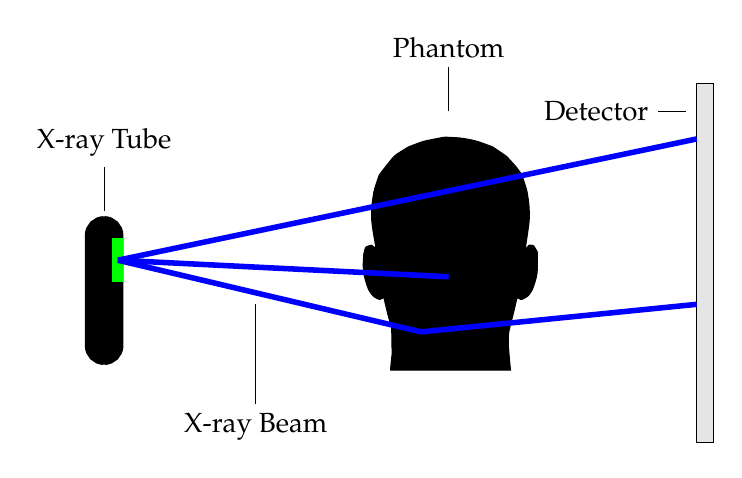
\begin{tikzpicture}[scale=.07]
        \draw[fill=black, rounded corners=5pt, line width=4] (-50,-40) rectangle (-45,-15);
        \draw[draw=green, line width=4] (-45,-18) -- (-45,-26);

        
        \draw[fill=gray!20] (60,10) rectangle (63,-55);
        
        \draw[fill=black]
        (349.5pt, -1.599976pt) .. controls (310.3pt, -9.299927pt) and (295pt,
        -12.79993pt) .. (287.5pt, -15.59998pt) -- (287.5pt, -15.59998pt) --
        (287.5pt, -15.59998pt) -- (287.5pt, -15.59998pt) .. controls (261.5pt,
        -25.09998pt) and (221.4pt, -40.19995pt) .. (219.6pt, -41.19995pt) --
        (219.6pt, -41.19995pt) -- (219.6pt, -41.19995pt) -- (219.6pt,
        -41.19995pt) .. controls (216.9pt, -42.59998pt) and (168.1pt, -73pt) ..
        (156.8pt, -80.29993pt) -- (156.8pt, -80.29993pt) -- (156.8pt,
        -80.29993pt) -- (156.8pt, -80.29993pt) .. controls (149.5pt, -85pt) and
        (146.4pt, -88pt) .. (138pt, -98.09998pt) -- (138pt, -98.09998pt) --
        (138pt, -98.09998pt) -- (138pt, -98.09998pt) .. controls (116.2pt,
        -124.2999pt) and (79.00001pt, -171.4999pt) .. (69.3pt, -185.4999pt) --
        (69.3pt, -185.4999pt) -- (69.3pt, -185.4999pt) -- (69.3pt, -185.4999pt)
        .. controls (67.3pt, -188.2999pt) and (50.10001pt, -239.1pt) .. (44.5pt,
        -258.4999pt) -- (44.5pt, -258.4999pt) -- (44.5pt, -258.4999pt) --
        (44.5pt, -258.4999pt) .. controls (40.3pt, -273.2pt) and (32.9pt,
        -320.7pt) .. (30.9pt, -345.9999pt) -- (30.9pt, -345.9999pt) -- (30.9pt,
        -345.9999pt) -- (30.9pt, -345.9999pt) .. controls (30.3pt, -353.9999pt)
        and (29.7pt, -374.2pt) .. (29.7pt, -390.9999pt) -- (29.7pt, -390.9999pt)
        -- (29.7pt, -390.9999pt) -- (29.7pt, -390.9999pt) .. controls (29.6pt,
        -418.2pt) and (29.9pt, -423.9pt) .. (32.2pt, -443.6pt) -- (32.2pt,
        -443.6pt) -- (32.2pt, -443.6pt) -- (32.2pt, -443.6pt) .. controls
        (33.7pt, -455.7pt) and (37.8pt, -482.1pt) .. (41.4pt, -502.1pt) --
        (41.4pt, -502.1pt) -- (41.4pt, -502.1pt) -- (41.4pt, -502.1pt) ..
        controls (49.10001pt, -544.8pt) and (51pt, -556.7pt) .. (51pt, -563.4pt)
        -- (51pt, -563.4pt) -- (51pt, -563.4pt) -- (51pt, -563.4pt) -- (51pt,
        -568.4pt) -- (51pt, -568.4pt) -- (40.6pt, -558.1pt) -- (40.6pt,
        -558.1pt) -- (40.6pt, -558.1pt) -- (40.6pt, -558.1pt) .. controls (29pt,
        -546.7pt) and (31.3pt, -547.4pt) .. (17.2pt, -551.1pt) -- (17.2pt,
        -551.1pt) -- (17.2pt, -551.1pt) -- (17.2pt, -551.1pt) .. controls
        (8.200001pt, -553.4999pt) and (0.500001pt, -557.3pt) .. (-1.499999pt,
        -560.3pt) -- (-1.499999pt, -560.3pt) -- (-1.499999pt, -560.3pt) --
        (-1.499999pt, -560.3pt) .. controls (-3.4pt, -563.2pt) and (-8.7pt,
        -580.7pt) .. (-10.5pt, -590.3pt) -- (-10.5pt, -590.3pt) -- (-10.5pt,
        -590.3pt) -- (-10.5pt, -590.3pt) .. controls (-11.3pt, -594.3pt) and
        (-12.5pt, -610.9pt) .. (-13.2pt, -627.3pt) -- (-13.2pt, -627.3pt) --
        (-13.2pt, -627.3pt) -- (-13.2pt, -627.3pt) -- (-14.4pt, -657.1pt) --
        (-14.4pt, -657.1pt) -- (-11.1pt, -683.8pt) -- (-11.1pt, -683.8pt) --
        (-11.1pt, -683.8pt) -- (-11.1pt, -683.8pt) .. controls (-7.4pt,
        -712.8pt) and (-5.099999pt, -723.2pt) .. (4.400002pt, -751.5pt) --
        (4.400002pt, -751.5pt) -- (4.400002pt, -751.5pt) -- (4.400002pt,
        -751.5pt) .. controls (14.6pt, -781.8pt) and (17.2pt, -786.9pt) ..
        (30.8pt, -803.4pt) -- (30.8pt, -803.4pt) -- (30.8pt, -803.4pt) --
        (30.8pt, -803.4pt) .. controls (38.2pt, -812.5pt) and (43.2pt, -816.3pt)
        .. (56.5pt, -823pt) -- (56.5pt, -823pt) -- (56.5pt, -823pt) -- (56.5pt,
        -823pt) .. controls (71.00001pt, -830.3pt) and (71.7pt, -830.3pt) ..
        (82.4pt, -823.5pt) -- (82.4pt, -823.5pt) -- (82.4pt, -823.5pt) --
        (82.4pt, -823.5pt) .. controls (89.2pt, -819.1pt) and (91.40001pt,
        -818.1pt) .. (92.10001pt, -819.2pt) -- (92.10001pt, -819.2pt) --
        (92.10001pt, -819.2pt) -- (92.10001pt, -819.2pt) .. controls
        (92.90001pt, -820.4pt) and (94.60001pt, -827.3pt) .. (107.5pt, -882pt)
        -- (107.5pt, -882pt) -- (107.5pt, -882pt) -- (107.5pt, -882pt) ..
        controls (115.6pt, -916.2pt) and (119.4pt, -930.2pt) .. (126.5pt,
        -952pt) -- (126.5pt, -952pt) -- (126.5pt, -952pt) -- (126.5pt, -952pt)
        -- (132.8pt, -971.5pt) -- (132.8pt, -971.5pt) -- (134pt, -1040.5pt) --
        (134pt, -1040.5pt) -- (135.1pt, -1109.5pt) -- (135.1pt, -1109.5pt) --
        (131.1pt, -1149.1pt) -- (131.1pt, -1149.1pt) -- (131.1pt, -1149.1pt) --
        (131.1pt, -1149.1pt) .. controls (128.8pt, -1170.9pt) and (127pt,
        -1189.7pt) .. (127pt, -1190.9pt) -- (127pt, -1190.9pt) -- (127pt,
        -1190.9pt) -- (127pt, -1190.9pt) -- (127pt, -1193pt) -- (127pt, -1193pt)
        -- (436.5pt, -1193pt) -- (436.5pt, -1193pt) -- (746.0001pt, -1193pt) --
        (746.0001pt, -1193pt) -- (745.5001pt, -1189.3pt) -- (745.5001pt,
        -1189.3pt) -- (745.5001pt, -1189.3pt) -- (745.5001pt, -1189.3pt) ..
        controls (744.0001pt, -1177.4pt) and (737.3pt, -1102pt) .. (735.4pt,
        -1075.5pt) -- (735.4pt, -1075.5pt) -- (735.4pt, -1075.5pt) -- (735.4pt,
        -1075.5pt) .. controls (733.4pt, -1047.1pt) and (733.9pt, -1024.6pt) ..
        (737.0001pt, -996pt) -- (737.0001pt, -996pt) -- (737.0001pt, -996pt) --
        (737.0001pt, -996pt) .. controls (739.5001pt, -972.6pt) and (740.1pt,
        -969.7pt) .. (748.0001pt, -946pt) -- (748.0001pt, -946pt) --
        (748.0001pt, -946pt) -- (748.0001pt, -946pt) .. controls (754.0001pt,
        -928.2pt) and (758.0001pt, -912.4pt) .. (771.1pt, -855.5pt) -- (771.1pt,
        -855.5pt) -- (771.1pt, -855.5pt) -- (771.1pt, -855.5pt) .. controls
        (778.4pt, -823.6pt) and (779.7pt, -819pt) .. (781.3pt, -819pt) --
        (781.3pt, -819pt) -- (781.3pt, -819pt) -- (781.3pt, -819pt) .. controls
        (782.0001pt, -819pt) and (785.3pt, -820.6pt) .. (788.6pt, -822.6pt) --
        (788.6pt, -822.6pt) -- (788.6pt, -822.6pt) -- (788.6pt, -822.6pt) ..
        controls (799.4pt, -829.3pt) and (799.7pt, -829.4pt) .. (804.4pt,
        -828pt) -- (804.4pt, -828pt) -- (804.4pt, -828pt) -- (804.4pt, -828pt)
        .. controls (810.3pt, -826.3pt) and (825.2001pt, -818.4pt) .. (831.8pt,
        -813.5pt) -- (831.8pt, -813.5pt) -- (831.8pt, -813.5pt) -- (831.8pt,
        -813.5pt) .. controls (839.3pt, -808.1pt) and (852.1pt, -791.1pt) ..
        (857.6pt, -779.5pt) -- (857.6pt, -779.5pt) -- (857.6pt, -779.5pt) --
        (857.6pt, -779.5pt) .. controls (862.1pt, -769.9pt) and (873.3pt,
        -736.7pt) .. (877.4pt, -721pt) -- (877.4pt, -721pt) -- (877.4pt, -721pt)
        -- (877.4pt, -721pt) .. controls (878.7001pt, -715.8pt) and (881.0001pt,
        -703.8pt) .. (882.4pt, -694.3pt) -- (882.4pt, -694.3pt) -- (882.4pt,
        -694.3pt) -- (882.4pt, -694.3pt) .. controls (884.9pt, -677.7pt) and
        (885.0001pt, -675.5pt) .. (885.0001pt, -632pt) -- (885.0001pt, -632pt)
        -- (885.0001pt, -632pt) -- (885.0001pt, -632pt) -- (885.0001pt,
        -586.8pt) -- (885.0001pt, -586.8pt) -- (881.0001pt, -576.7pt) --
        (881.0001pt, -576.7pt) -- (881.0001pt, -576.7pt) -- (881.0001pt,
        -576.7pt) .. controls (877.2001pt, -567.1pt) and (875.4pt, -564.2pt) ..
        (867.1pt, -554.2pt) -- (867.1pt, -554.2pt) -- (867.1pt, -554.2pt) --
        (867.1pt, -554.2pt) .. controls (863.5001pt, -549.8pt) and (862.9pt,
        -549.6pt) .. (848.9pt, -548.6pt) -- (848.9pt, -548.6pt) -- (848.9pt,
        -548.6pt) -- (848.9pt, -548.6pt) -- (842.3pt, -548.1pt) -- (842.3pt,
        -548.1pt) -- (834.4pt, -556.1pt) -- (834.4pt, -556.1pt) -- (834.4pt,
        -556.1pt) -- (834.4pt, -556.1pt) .. controls (830.1pt, -560.4999pt) and
        (825.3pt, -564.9999pt) .. (823.8pt, -566.1pt) -- (823.8pt, -566.1pt) --
        (823.8pt, -566.1pt) -- (823.8pt, -566.1pt) .. controls (821.4pt,
        -567.8pt) and (821.2001pt, -567.9pt) .. (821.6pt, -566.3pt) -- (821.6pt,
        -566.3pt) -- (821.6pt, -566.3pt) -- (821.6pt, -566.3pt) .. controls
        (823.1pt, -559.7pt) and (836.5001pt, -470.9pt) .. (839.0001pt,
        -450.9999pt) -- (839.0001pt, -450.9999pt) -- (839.0001pt, -450.9999pt)
        -- (839.0001pt, -450.9999pt) .. controls (843.3pt, -415.4pt) and
        (843.8pt, -406.4999pt) .. (842.9pt, -377.9999pt) -- (842.9pt,
        -377.9999pt) -- (842.9pt, -377.9999pt) -- (842.9pt, -377.9999pt) ..
        controls (841.8pt, -344.7pt) and (840.7001pt, -332.9pt) .. (835.9pt,
        -301.1pt) -- (835.9pt, -301.1pt) -- (835.9pt, -301.1pt) -- (835.9pt,
        -301.1pt) .. controls (830.4pt, -264.7999pt) and (831.3pt, -268.4pt) ..
        (815.5001pt, -219.9pt) -- (815.5001pt, -219.9pt) -- (815.5001pt,
        -219.9pt) -- (815.5001pt, -219.9pt) -- (805.2001pt, -188.4pt) --
        (805.2001pt, -188.4pt) -- (794.7pt, -171.9pt) -- (794.7pt, -171.9pt) --
        (794.7pt, -171.9pt) -- (794.7pt, -171.9pt) .. controls (788.8pt,
        -162.8999pt) and (780.5001pt, -151.2pt) .. (776.2pt, -146pt) --
        (776.2pt, -146pt) -- (776.2pt, -146pt) -- (776.2pt, -146pt) .. controls
        (769.8pt, -138.2pt) and (745.9pt, -112pt) .. (726.5001pt, -91.29993pt)
        -- (726.5001pt, -91.29993pt) -- (726.5001pt, -91.29993pt) --
        (726.5001pt, -91.29993pt) .. controls (724.3pt, -89pt) and (706.8pt,
        -76.69995pt) .. (687.5001pt, -63.8999pt) -- (687.5001pt, -63.8999pt) --
        (687.5001pt, -63.8999pt) -- (687.5001pt, -63.8999pt) -- (652.6pt,
        -40.69995pt) -- (652.6pt, -40.69995pt) -- (626.0001pt, -30.79993pt) --
        (626.0001pt, -30.79993pt) -- (626.0001pt, -30.79993pt) -- (626.0001pt,
        -30.79993pt) .. controls (585.2pt, -15.49988pt) and (570pt, -10.69995pt)
        .. (545pt, -5.499878pt) -- (545pt, -5.499878pt) -- (545pt, -5.499878pt)
        -- (545pt, -5.499878pt) .. controls (512.4pt, 1.200073pt) and (497pt,
        3.800049pt) .. (481.9pt, 5.000122pt) -- (481.9pt, 5.000122pt) --
        (481.9pt, 5.000122pt) -- (481.9pt, 5.000122pt) .. controls (460.8pt,
        6.600098pt) and (415.2pt, 9.000122pt) .. (408pt, 8.900024pt) -- (408pt,
        8.900024pt) -- (408pt, 8.900024pt) -- (408pt, 8.900024pt) .. controls
        (404.2pt, 8.800049pt) and (380pt, 4.500122pt) .. (349.5pt, -1.599976pt)
        -- cycle ;
        \draw[blue, line width=2] (-45,-22) -- (60,0);
        \draw[blue, line width=2] (-45,-22) -- (10,-35);
        \draw[blue, line width=2] (-45,-22) -- (15,-25);
        \draw[blue, line width=2] (10,-35) -- (60,-30);

        \draw (-47.5,-13) -- (-47.5,-5) node[above] {X-ray Tube};
        \draw (15,5) -- (15,13) node[above] {Phantom};
        \draw (58,5) -- (53,5) node [left] {Detector};
        \draw (-20,-30) -- (-20,-48) node[below] {X-ray Beam};
    \end{tikzpicture}
    \caption{Schematic illustration of photon transport in X-ray imaging.}
    \label{fig:photon_transport}
\end{figure}

In a typical simulation workflow, individual photons are emitted from the X-ray
tube and propagate through air before reaching the phantom. Upon entering the
phantom, they may interact with the material through scattering or absorption,
depending on the local composition of the tissue and photon energy. Only a
fraction of the photons will exit the phantom, continue their path through air,
and ultimately reach the detector, contributing to the final image formation.

The simulation framework described here forms the basis for all subsequent
analyses presented in this thesis.


%-------------------------------------------------------------------------------%	SECTION 2
\section{X-Ray Tube}
%-------------------------------------------------------------------------------

X-ray beams are generated within evacuated glass tubes containing several
critical components that convert electrical energy into X-ray photons and heat.
The X-ray tube acts as an energy converter, where the vast majority of the input
energy is transformed into heat and only a small fraction becomes useful
radiation. The following Figure~\ref{fig:xray_tube} illustrates the basic
construction of an X-ray tube as in \cite{poludniowski2022calculating}

\begin{figure}[htbp]
    \centering
    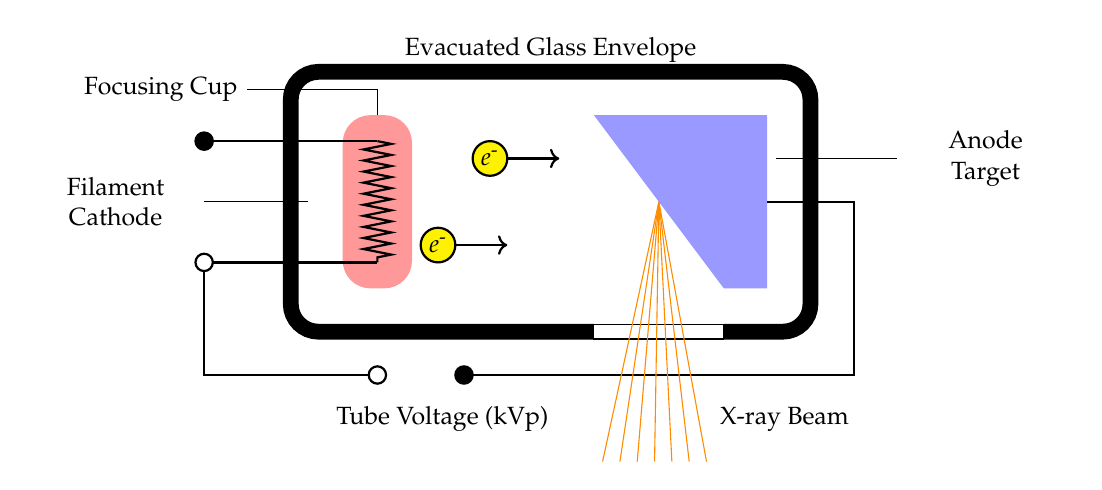
\begin{tikzpicture}[scale=1.1, every node/.style={font=\small}]
        % Glass envelope
        \draw[line width=2mm, rounded corners=10pt] (.5,-1.5) -- (-3,-1.5) -- (-3,1.5) -- (3,1.5) -- (3,-1.5) -- (2,-1.5);
        % Optional: dashed or lighter line to indicate the open section
        \draw (0.5,-1.415) rectangle (2,-1.585);
        \node[above] at (0,1.5) {Evacuated Glass Envelope};
        
        % Focusing Cup
        \draw[rounded corners=10pt, fill=red!40, draw=none] (-2.4,1) rectangle (-1.6,-1);
        \draw (-2,1) -- (-2,1.3) -- (-3.5,1.3) node [left] {Focusing Cup};

        % Filament (cathode)
        \draw[thick] (-4,.7) -- (-2,.7);
        \draw[thick, fill=black] (-4,.7) circle [radius=0.1];
        \draw[thick] (-4,-.7) -- (-2,-.7);
        \draw[thick] (-2,-2) -- (-4,-2) -- (-4,-.7);
        \draw[thick, fill=white] (-4,-.7) circle [radius=0.1];
        \draw[thick, decorate, decoration={zigzag, segment length=4pt, 
        amplitude=5pt}] (-2,.7) -- (-2,-.7);
        \draw (-2.8,0) -- (-4,0) node[left, align=center, text width=2cm] {Filament\\Cathode};

        % Anode Target
        \draw[fill=blue!40, draw=none] (.5,1) -- (2.5,1) -- (2.5,-1) -- (2,-1) -- cycle;
        \draw (2.6,.5) -- (4,.5) node[right, align=center, text width=2cm] {Anode\\Target};

        % Anode Voltage
        \draw[thick] (2.5,0) -- (3.5,0) -- (3.5,-2) -- (-1,-2);
        \draw[thick, fill=black] (-1,-2) circle [radius=0.1];
        \draw[thick, fill=white] (-2,-2) circle [radius=0.1];
        \node[below, align=center, text height=.5cm] at (-1.25,-2) {Tube Voltage (kVp)};

        % Electrons
        \draw[thick,->] (-1.3,-.5) -- (-.5,-.5);
        \draw[thick, fill=yellow] (-1.3,-.5) circle [radius=0.2] node[font=\small] {$e^{\text{-}}$};
        \draw[thick,->] (-.7,.5) -- (.1,.5);
        \draw[thick, fill=yellow] (-.7,.5) circle [radius=0.2] node[font=\small] {$e^{\text{-}}$};

        % Photon Beam
        \draw[orange!90!yellow] (.6,-3) -- (1.25,0);
        \draw[orange!90!yellow] (.8,-3) -- (1.25,0);
        \draw[orange!90!yellow] (1,-3) -- (1.25,0);
        \draw[orange!90!yellow] (1.2,-3) -- (1.25,0);
        \draw[orange!90!yellow] (1.4,-3) -- (1.25,0);
        \draw[orange!90!yellow] (1.6,-3) -- (1.25,0);
        \draw[orange!90!yellow] (1.8,-3) -- (1.25,0);
        \node[right, below, align=center, text height=.5cm] at (2.7,-2) {X-ray Beam};
    \end{tikzpicture}
    \caption{Schematic of an X-ray tube.}
    \label{fig:xray_tube}
\end{figure}


\subsection{Photon Generation}

To capture this randomness, Monte Carlo methods
are employed. In such simulations, random numbers—typically sampled uniformly
from the interval $[0,1]$ are transformed into physically meaningful
quantities according to the relevant probability distributions. This
probabilistic modeling enables realistic simulation of photon transport and
forms the basis for the analyses presented in this thesis.



The key components are:

\begin{itemize}
    \item \textbf{Filament (Cathode):} A tungsten wire filament serves as the
    electron source through thermionic emission. When a current of approximately
    3-6\,A passes through it, the filament reaches incandescence, releasing
    electrons from its surface. These free electrons form a cloud near the
    cathode until they are accelerated toward the anode by the applied high
    voltage.

    \item \textbf{Focusing Cup:} The filament is embedded in a negatively
    charged, nickel-made focusing cup. Its function is to electrostatically
    shape and direct the electron stream toward the anode’s focal spot, thereby
    influencing the resolution and size of the resulting X-ray beam.

    \item \textbf{Anode Target:} The anode consists of a tungsten target, often
    embedded in a copper support. Tungsten is used for its high atomic number
    and melting point, enhancing X-ray production and durability. The copper
    base improves heat dissipation. Typically, less than 1\% of the electron
    energy is converted into X-rays, with the remainder generating heat that
    must be effectively managed.

    \item \textbf{Evacuated Glass Envelope:} All components are sealed within a
    borosilicate glass or metal-ceramic housing evacuated to a low pressure
    (typically $10^{-5}$ to $10^{-7}$\,hPa). The vacuum allows unimpeded
    electron flow and prevents arcing. The housing is usually immersed in
    insulating oil to provide thermal and electrical isolation.
\end{itemize}

When high-energy electrons strike the tungsten target, X-ray photons are
produced through two primary mechanisms:

\begin{itemize}
    \item \textbf{Bremsstrahlung (Braking Radiation):} This accounts for
    approximately 80\% of X-ray production. When electrons pass close to
    tungsten nuclei, they are decelerated by the electrostatic attraction,
    causing them to lose kinetic energy that is emitted as X-ray photons. This
    process produces a continuous spectrum of X-ray energies from near zero up
    to the maximum electron energy.

    \item \textbf{Characteristic Radiation:} This occurs when high-energy
    electrons knock inner shell electrons from tungsten atoms. When outer shell
    electrons drop down to fill these vacancies, they emit X-rays with discrete,
    characteristic energies specific to tungsten. Therefore peaks are occuring
    at the difference of the binding energies of the electron shells. For
    reference, the atomic model of tungsten is given in
    Figure~\ref{fig:tungsten_atomic_model} and the approximate binding energies
    of the electron shells in Table~\ref{tab:tungsten_binding_energies}.

    \begin{table}[!h]
        \centering
        \begin{tabular}{cc}
            \toprule
            \textbf{Shell / Subshell} & \textbf{Binding Energy (keV)} \\
            \midrule
            K        & 69.5 \\
            L$_1$    & 12.1 \\
            L$_2$    & 11.5 \\
            L$_3$    & 10.2 \\
            M$_1$    & 2.82 \\
            M$_2$    & 2.30 \\
            M$_3$    & 2.15 \\
            N$_1$    & 0.43 \\
            N$_2$    & 0.32 \\
            N$_3$    & 0.22 \\
            \bottomrule
        \end{tabular}
        \caption{Approximate Electron Binding Energies of Tungsten (W, Z = 74)}
        \label{tab:tungsten_binding_energies}
    \end{table}

    % TODO: W und Z sollten als Abkürzungen in \ac{acronym} definiert werden

    \begin{figure}
        \centering
        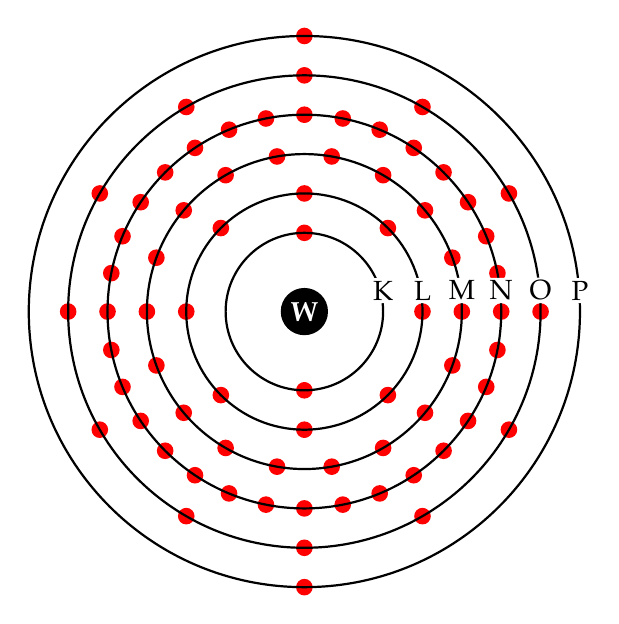
\begin{tikzpicture}[scale=1]
            % Kern
            \fill[black] (0,0) circle (0.3);
            \node at (0,0) [white] {\textbf{W}};

            % Elektronen (vereinfacht verteilt)
            % K-Schale: 2
            \foreach \angle in {90, 270} {
                \fill[color=red] (0,0) ++(\angle:1) circle (3pt);
            }

            % L-Schale: 8
            \foreach \angle in {0, 45, 90, 135, 180, 225, 270, 315} {
                \fill[color=red] (0,0) ++(\angle:1.5) circle (3pt);
            }

            % M-Schale: 18
            \foreach \angle in {0, 20, 40, 60, 80, 100, 120, 140, 160, 180, 200, 220, 240, 260, 280, 300, 320, 340} {
                \fill[color=red] (0,0) ++(\angle:2cm) circle (3pt);
            }

            % N-Schale: 32
            \foreach \angle in {0,11.25,...,348.75} {
                \fill[color=red] (0,0) ++(\angle:2.5cm) circle (3pt);
            }

            % O-Schale: 12
            \foreach \angle in {0,30,...,330} {
                \fill[color=red] (0,0) ++(\angle:3cm) circle (3pt);
            }

            % P-Schale: 2
            \foreach \angle in {90, 270} {
                \fill[color=red] (0,0) ++(\angle:3.5cm) circle (3pt);
            }
            
            % Schalen
            \foreach \radius/\label in {
                1/K,
                1.5/L,
                2/M,
                2.5/N,
                3/O,
                3.5/P
            } {
                \draw[thick] (0,0) circle (\radius);
                \node[above, fill=white, inner sep=1pt, rounded corners=1pt] at (\radius, 0.1) {\label};
            }
        \end{tikzpicture}
        \caption{Bohr model of the tungsten atom (W, Z = 74) with electron shells and subshells.}
        \label{fig:tungsten_atomic_model}
    \end{figure}

    In Table~\ref{tab:tungsten_binding_energies} only binding energies of the K,
    L and M shells are given, since these are the most relevant for X-ray
    production. The binding energies of the N shell and higher shells are
    negligible in this context due to their low binding energies.   
    
\end{itemize}

Although it is not necessary to understand every technical detail of the X-ray
apparatus for the purposes of simulation, I found it important to briefly
present the fundamental working principles of the X-ray tube. This background
allows one to appreciate how key simulation parameters for photon generation -
specifically the tube voltage and the cathode material - influence the resulting
X-ray spectrum and photon behavior.

Figure~\ref{fig:spectrum100kvp} below shows an resulting energy spectrum for an
X-ray tube with a tungsten cathode operated at 100 kVp. It illustrates the
resulting distribution of photon energies, which is shaped by both the material
and the applied voltage. The intensity of the different photon energies is
measured in \emph{spectral fluence} in
\si{\per\square\centi\meter\per\kilo\electronvolt}, which describes the number
of X-ray photons per unit area per unit energy interval. It certainly shows the
two components of the X-ray spectrum: the continuous bremsstrahlung spectrum and
the characteristic radiation peaks:

\begin{figure}[H]
    \centering
    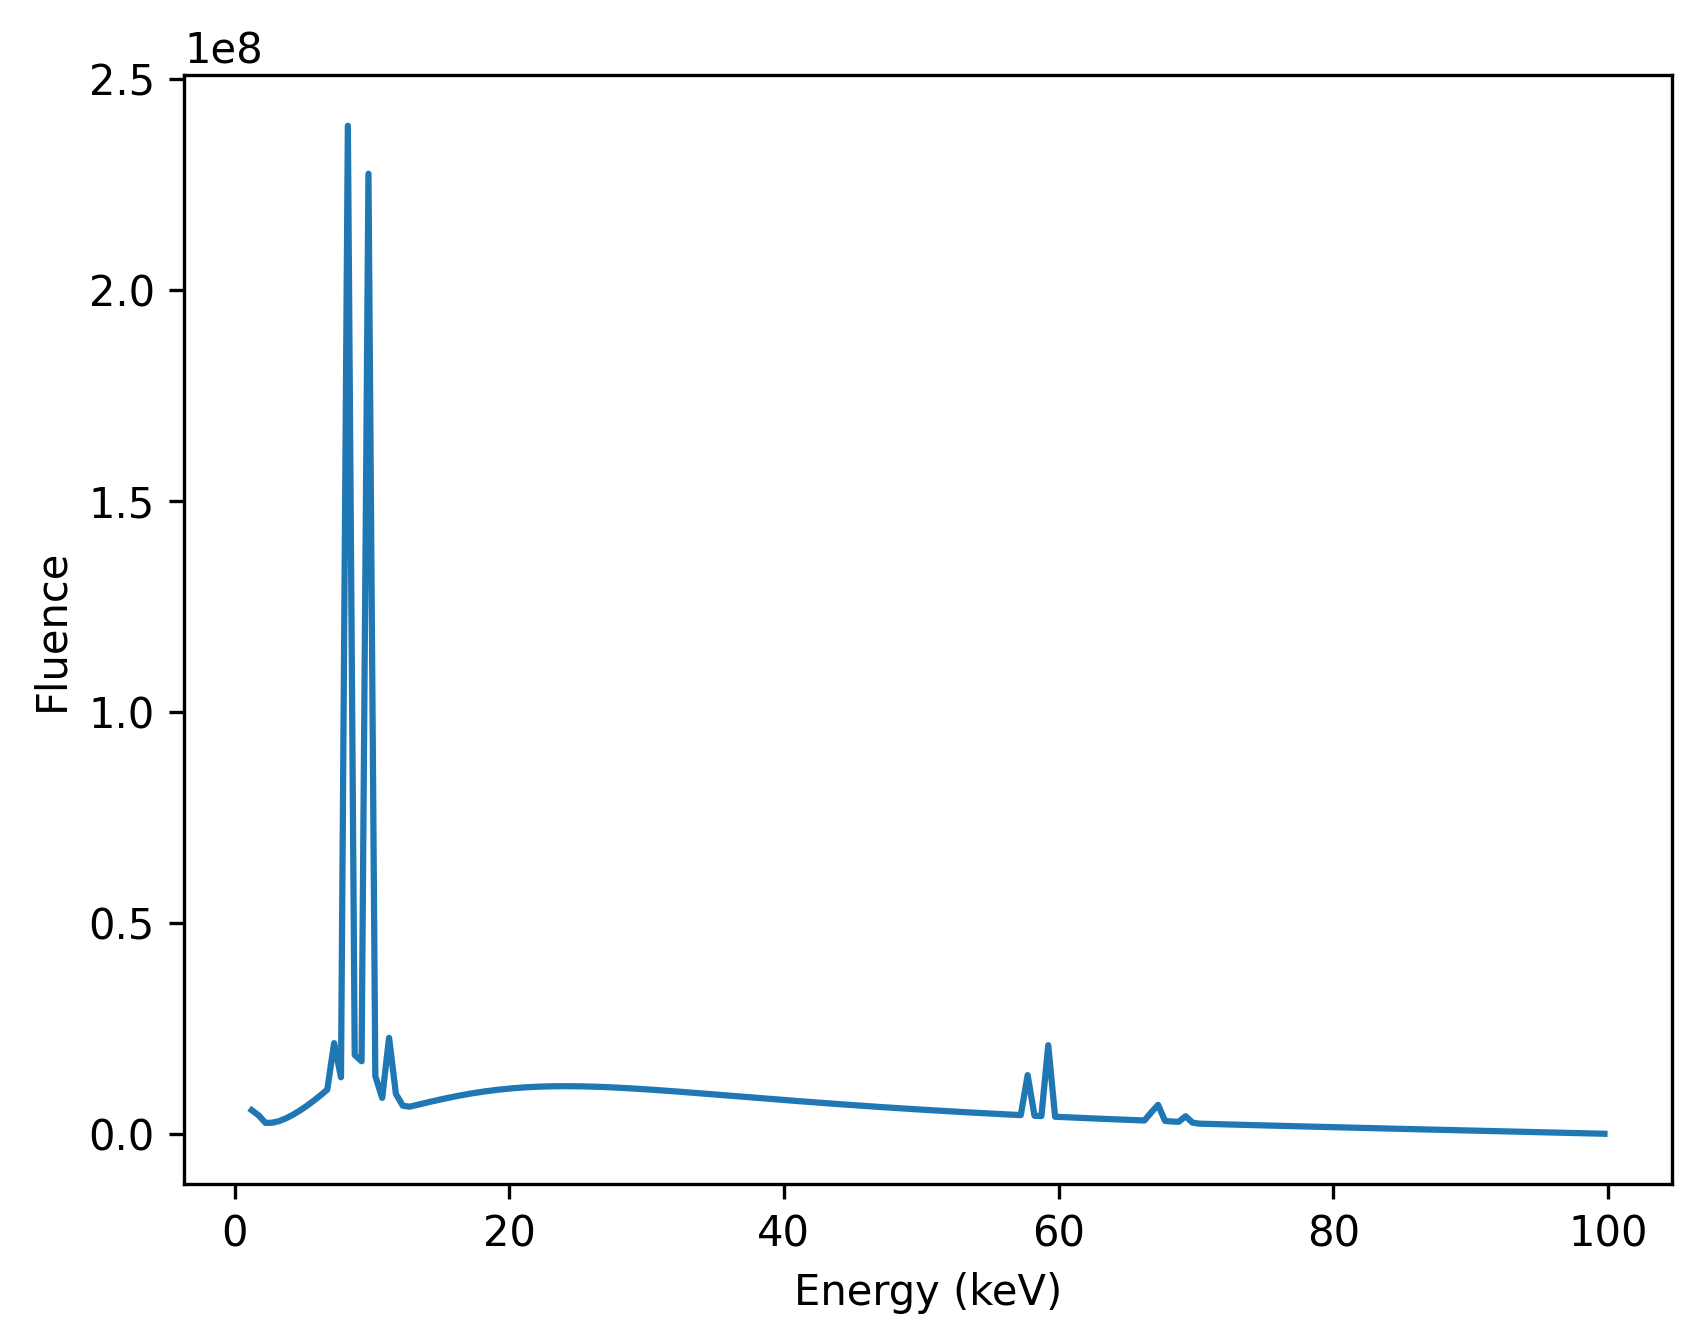
\includegraphics[width=0.8\textwidth]{Figures/spectrum_without_filter.png}
    \caption{X-ray spectrum for a tungsten cathode at 100 kVp showing the
    continuous bremsstrahlung spectrum and characteristic peaks. Build with
    \emph{SpekPy} \cite{spekpy}}
    \label{fig:spectrum100kvp}
\end{figure}


\subsection{Filter}
\label{sec:filter}

Low energy X-ray photons contribute little to image formation but significantly
increase patient dose. Therefore, X-ray tubes are often equipped with filters to
selectively attenuate these low-energy photons while allowing higher-energy
photons to pass through. This process, known as beam hardening, improves image
quality by reducing scatter and enhancing contrast. Common filter materials
include aluminum, copper and molybdenum, which are chosen based on their atomic
number and thickness to effectively absorb low-energy photons while minimizing
the impact on higher-energy photons \cite{poludniowski2022calculating}.

As can be seen in Figure~\ref{fig:xray_tube_with_filter}, the filter is placed
at the X-ray tube margin such that the photons hit the filter after the anode
target and before leaving the X-ray tube. Followingly X-rays pass through the
filter before reaching the patient.

\begin{figure}[H]
    \centering
    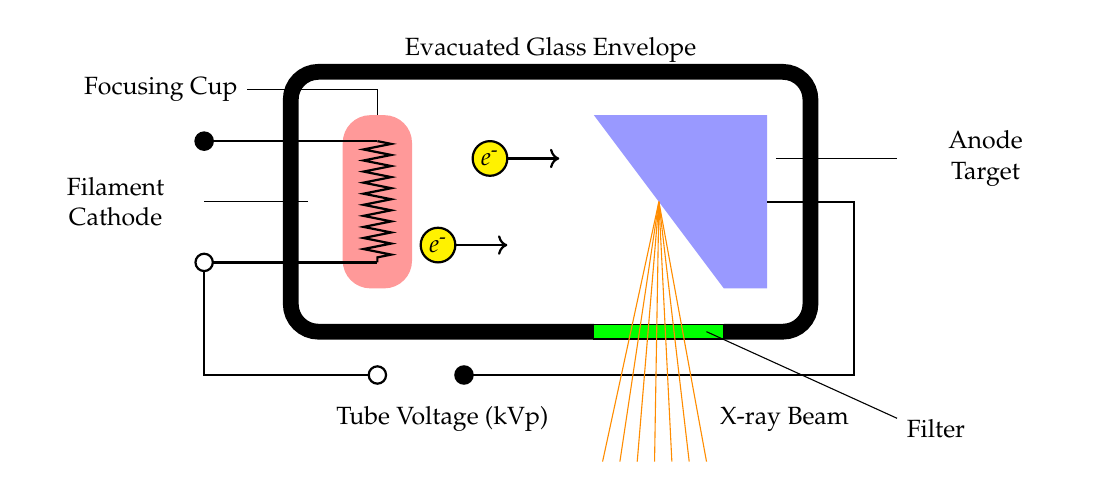
\begin{tikzpicture}[scale=1.1, every node/.style={font=\small}]
        % Glass envelope
        \draw[line width=2mm, rounded corners=10pt] (.5,-1.5) -- (-3,-1.5) -- (-3,1.5) -- (3,1.5) -- (3,-1.5) -- (2,-1.5);
        % Optional: dashed or lighter line to indicate the open section
        \draw[fill=green] (0.5,-1.415) rectangle (2,-1.585);
        \node[above] at (0,1.5) {Evacuated Glass Envelope};
        
        % Focusing Cup
        \draw[rounded corners=10pt, fill=red!40, draw=none] (-2.4,1) rectangle (-1.6,-1);
        \draw (-2,1) -- (-2,1.3) -- (-3.5,1.3) node [left] {Focusing Cup};

        % Filament (cathode)
        \draw[thick] (-4,.7) -- (-2,.7);
        \draw[thick, fill=black] (-4,.7) circle [radius=0.1];
        \draw[thick] (-4,-.7) -- (-2,-.7);
        \draw[thick] (-2,-2) -- (-4,-2) -- (-4,-.7);
        \draw[thick, fill=white] (-4,-.7) circle [radius=0.1];
        \draw[thick, decorate, decoration={zigzag, segment length=4pt, 
        amplitude=5pt}] (-2,.7) -- (-2,-.7);
        \draw (-2.8,0) -- (-4,0) node[left, align=center, text width=2cm] {Filament\\Cathode};

        % Anode Target
        \draw[fill=blue!40, draw=none] (.5,1) -- (2.5,1) -- (2.5,-1) -- (2,-1) -- cycle;
        \draw (2.6,.5) -- (4,.5) node[right, align=center, text width=2cm] {Anode\\Target};

        % Anode Voltage
        \draw[thick] (2.5,0) -- (3.5,0) -- (3.5,-2) -- (-1,-2);
        \draw[thick, fill=black] (-1,-2) circle [radius=0.1];
        \draw[thick, fill=white] (-2,-2) circle [radius=0.1];
        \node[below, align=center, text height=.5cm] at (-1.25,-2) {Tube Voltage (kVp)};

        % Electrons
        \draw[thick,->] (-1.3,-.5) -- (-.5,-.5);
        \draw[thick, fill=yellow] (-1.3,-.5) circle [radius=0.2] node[font=\small] {$e^{\text{-}}$};
        \draw[thick,->] (-.7,.5) -- (.1,.5);
        \draw[thick, fill=yellow] (-.7,.5) circle [radius=0.2] node[font=\small] {$e^{\text{-}}$};

        % Photon Beam
        \draw[orange!90!yellow] (.6,-3) -- (1.25,0);
        \draw[orange!90!yellow] (.8,-3) -- (1.25,0);
        \draw[orange!90!yellow] (1,-3) -- (1.25,0);
        \draw[orange!90!yellow] (1.2,-3) -- (1.25,0);
        \draw[orange!90!yellow] (1.4,-3) -- (1.25,0);
        \draw[orange!90!yellow] (1.6,-3) -- (1.25,0);
        \draw[orange!90!yellow] (1.8,-3) -- (1.25,0);
        \node[right, below, align=center, text height=.5cm] at (2.7,-2) {X-ray Beam};
        \draw (1.8,-1.5) -- (4,-2.5) node[right, align=center, text height=.5cm] {Filter};
    \end{tikzpicture}
    \caption{Schematic of an X-ray tube with Filter.}
    \label{fig:xray_tube_with_filter}
\end{figure}

Throughout this thesis, a filter consisting of $0.4$ \si{\milli\meter} Tin (Sn)
and $0.1$ \si{\milli\meter} Copper (Cu) is used for the simulations. This filter
is chosen to represent a realistic X-ray tube filter that is commonly used in
clinical practice \cite{steidel2022dose}. The resulting spectrum is shown in
Figure~\ref{fig:spectrum100kvp_with_filter}.

\begin{figure}[H]
    \centering
    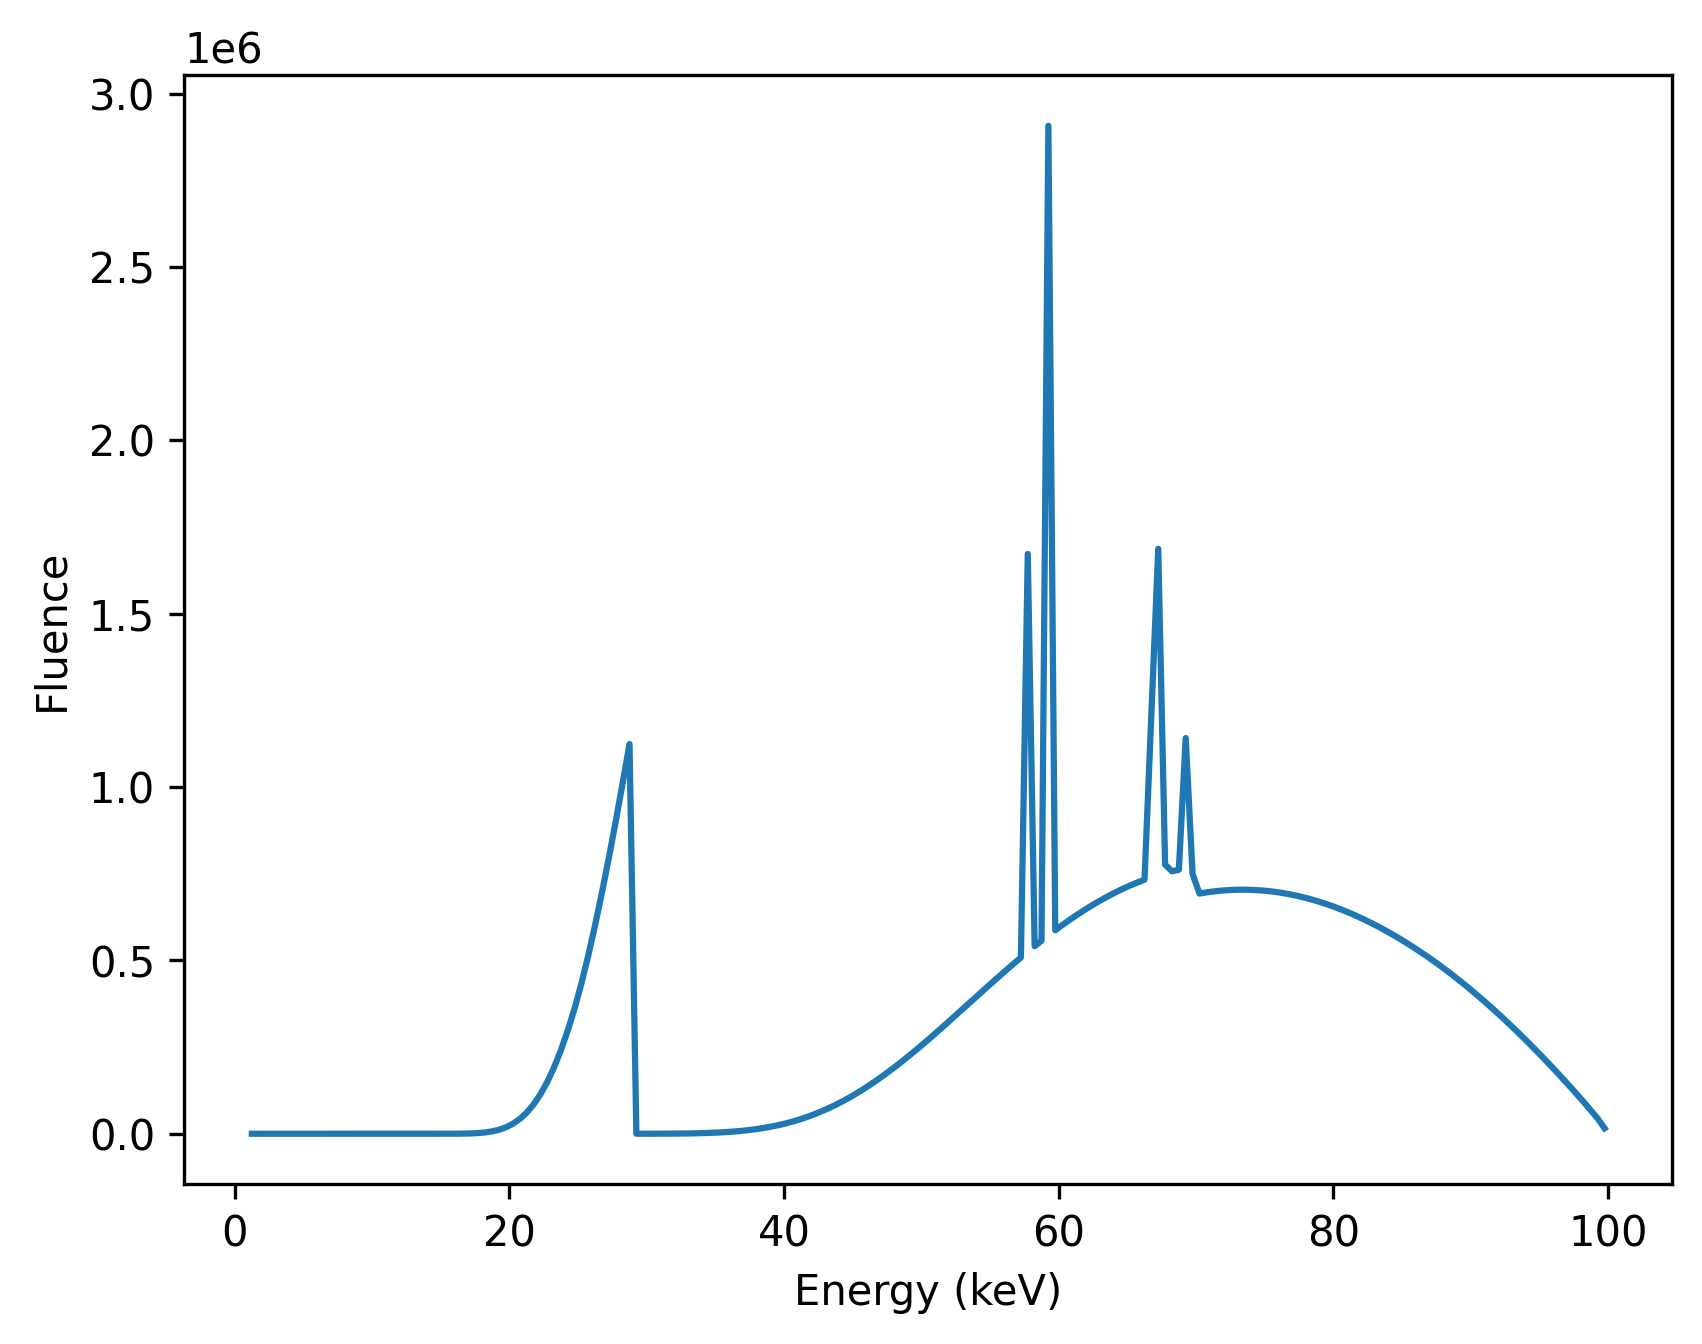
\includegraphics[width=0.8\textwidth]{Figures/spectrum_with_filter.png}
    \caption{X-ray spectrum for a tungsten cathode at $100$ \si{\kilo\voltpeak}
    with a $0.4$ \si{\milli\meter} showing the continuous bremsstrahlung
    spectrum and characteristic peaks. Build with \emph{SpekPy} \cite{spekpy}}
    \label{fig:spectrum100kvp_with_filter}
\end{figure}


%-------------------------------------------------------------------------------
%	SECTION 3
\section{Photon Generation}
%-------------------------------------------------------------------------------

In the context of Monte Carlo simulations, photons are generated from the X-ray
tube source, which is typically modeled as a point source emitting photons
within a conical beam. The emission cone is defined by a half-angle $\Theta$,
which determines the angular distribution of emitted photons. -- The emitted photons are characterized by two key properties: their direction and
energy. 

\subsection{Photon Energy}
\label{sec:photon_energy}
The photon energy is sampled from the X-ray tube spectrum as described in
Section~\ref{sec:filter}. In the simulations referenced in this thesis the
spectra are generated utilizing \emph{SpekPy} \cite{spekpy,
poludniowski2021spekpy}. The energies of the resulting photons are sampled via
inverse transform sampling from the normalized spectrum.

Inverse transform sampling \cite{muller2012monte} is a method to generate random samples from a target distribution using uniformly distributed random variables, such as those generated by a Quasi-Monte Carlo sequence.

\begin{definition}[Inverse Transform Sampling]\ \\
    \label{def:inverse_transform_sampling}
    Let $F_X: \mathbb{R} \to [0,1]$ be the cumulative distribution function (CDF) of a continuous, strictly increasing random variable $X$. The method of \emph{inverse transform sampling} generates a realization of $X$ by the following procedure:

    \begin{enumerate}
        \item Generate a sample $U$ from the uniform distribution on the unit interval, i.e., $U \sim \mathcal{U}(0,1)$.
        \item Compute the value $X := F_X^{-1}(U)$, where $F_X^{-1}$ denotes the inverse of the CDF $F_X$.
    \end{enumerate}
\end{definition}

\begin{theorem}\ \\
Let $F_X$ be a continuous and strictly increasing cumulative distribution function and let $U \sim \mathcal{U}(0,1)$. Then the random variable
\[
X := F_X^{-1}(U)
\]
has cumulative distribution function $F_X$, i.e.,
\[
\mathbb{P}(X \leq x) = F_X(x), \quad \text{for all } x \in \mathbb{R}.
\]
\end{theorem}

\begin{proof}\ \\
Since $F_X$ is continuous and strictly increasing, its inverse $F_X^{-1}$ exists. For any $x \in \mathbb{R}$, we compute:

\[
\mathbb{P}(X \leq x) = \mathbb{P}(F_X^{-1}(U) \leq x)
= \mathbb{P}(U \leq F_X(x)) \quad  \underset{\text{decreasing}}{\overset{\text{since } F_X \text{ is strictly}}{=}} F_X(x),
\]

because \( U \sim \mathcal{U}(0,1) \) and thus \( \mathbb{P}(U \leq u) = u \) for all \( u \in [0,1] \). This shows that \( X \) has CDF \( F_X \).
\end{proof}


\subsection{Photon Direction}
The direction of each emitted photon is sampled uniformly within a conical
emission cone defined by the half-angle $\Theta$. For the simulation a spherical alignment of the X-ray tube is assumed, such that the beam is oriented along the vector $\vec{v} = (v_1,v_2,v_3)$ in the Cartesian coordinate system.

Followingly, the direction of the emitted photon is sampled based on two random
values $u_1, u_2 \in [0,1)$ as follows:
\begin{enumerate}
    \item Sample a random angle $\theta$ uniformly from the interval $[0,
    \Theta]$ with $u_1$:
    $$\theta = u_1 \cdot \Theta$$
    \item Sample a random azimuthal angle $\phi$ uniformly from the interval
    $[0, 2\pi)$ with $u_2$:
    $$\phi = u_2 \cdot 2\pi$$
    \item Compute the direction vector $\vec{d}$ of the photon as:
    $$\vec{d} = (\sin(\theta) \cos(\phi), \sin(\theta) \sin(\phi),
    \cos(\theta))$$
\end{enumerate}


% ------------------------------------------------------------------------------
\section{Scattering and Attenuation}
%-------------------------------------------------------------------------------

This section provides the basic concepts of photon interaction with matter. The
interaction relevant for medical imaging results in a reduction of radiation
intensity, which corresponds to a decreased number of photons reaching the
detector. Hereby X-ray photons may be fully absorbed by \emph{photoelectric absorption} or undergo either \emph{elastic scattering} (Rayleigh) or \emph{inelastic scattering} (Compton) as they interact with matter.

The attenuation of X-ray photons arises from physical processes that alter their
number, direction, or energy as they interact with matter. These interactions
occur at the level of individual photons and are highly dependent on the photon
energy. This section presents an overview of the primary interaction mechanisms
relevant to attenuation like in \cite{medicalImagingSystemsIntro2019:}.

For correctness, in the simmulations it is further assumed that the X-ray
photons are propagating through vacuum before entering and after exiting the
phantom. Usually the tissues are surrounded by air, which has a negligible
effect on the photon transport.

\begin{figure}
    \centering
    \begin{minipage}[t]{0.45\textwidth}
        \raggedright
        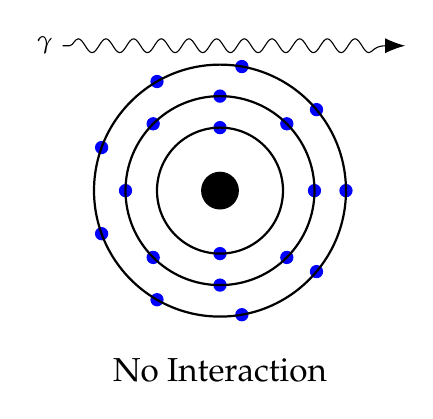
\begin{tikzpicture}[scale=.8]
            \draw[decorate, decoration=snake, {Latex[scale=1.5]}-, shorten <=-10] (2.5,2.3) -- (-2.5,2.3) node[left] {\small$\gamma$};
            \fill[black] (0,0) circle (0.3);
            \foreach \angle in {90, 270} {
                \fill[color=blue] (0,0) ++(\angle:1) circle (3pt);
            }
            \foreach \angle in {0, 45, 90, 135, 180, 225, 270, 315} {
                \fill[color=blue] (0,0) ++(\angle:1.5) circle (3pt);
            }
            \foreach \angle in {0, 40, 80, 120, 160, 200, 240, 280, 320} {
                \fill[color=blue] (0,0) ++(\angle:2cm) circle (3pt);
            }
            \foreach \radius in {1,1.5,2}
            {
                \draw[thick] (0,0) circle (\radius);
            }
            \node[below, font=\large] at (0,-2.5) {No Interaction};
        \end{tikzpicture}
    \end{minipage}
    \begin{minipage}[t]{0.45\textwidth}
        \raggedleft
        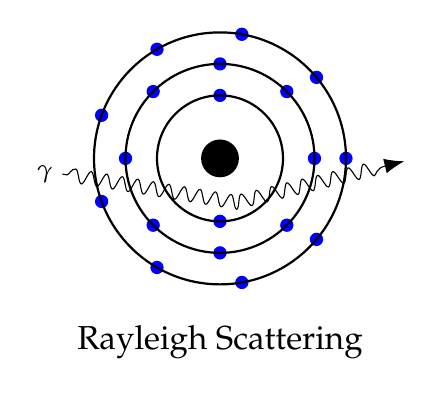
\begin{tikzpicture}[scale=.8]
            \draw[decorate, decoration=snake, segment length=2mm, {Latex[scale=1.5]}-, shorten <=-10] (2.5,-.15) -- (.25,-.7) -- (-2.5,-.25) node[left] {\small$\gamma$};
            \fill[black] (0,0) circle (0.3);
            \foreach \angle in {90, 270} {
                \fill[color=blue] (0,0) ++(\angle:1) circle (3pt);
            }
            \foreach \angle in {0, 45, 90, 135, 180, 225, 270, 315} {
                \fill[color=blue] (0,0) ++(\angle:1.5) circle (3pt);
            }
            \foreach \angle in {0, 40, 80, 120, 160, 200, 240, 280, 320} {
                \fill[color=blue] (0,0) ++(\angle:2cm) circle (3pt);
            }
            \foreach \radius in {1,1.5,2}
            {
                \draw[thick] (0,0) circle (\radius);
            }
            \node[below, font=\large] at (0,-2.5) {Rayleigh Scattering};
        \end{tikzpicture}
    \end{minipage}
    \par\vspace{2em}
    \begin{minipage}[t]{0.45\textwidth}
        \raggedright
        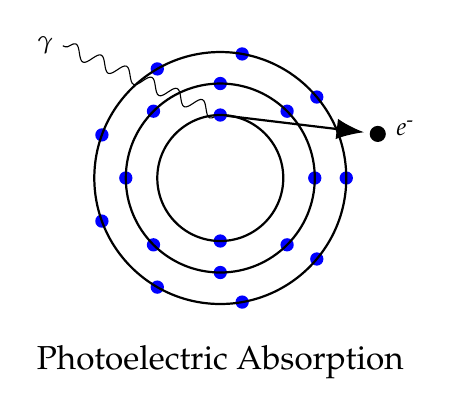
\begin{tikzpicture}[scale=.8]
            \draw[decorate, decoration=snake] (0,1) -- (-2.5,2.1) node[left] {\small$\gamma$};
            \draw[thick] [thick, -{Latex[scale=1.5]}, shorten >=5] (0,1) --
            (2.5, .7) node[draw, circle, fill=black, minimum size=5pt, inner
            sep=0pt] {} node[xshift=10pt, yshift=2pt] {\small$e^\text{-}$};
            \foreach \angle in {90, 270} {
                \fill[color=blue] (0,0) ++(\angle:1) circle (3pt);
            }
            \foreach \angle in {0, 45, 90, 135, 180, 225, 270, 315} {
                \fill[color=blue] (0,0) ++(\angle:1.5) circle (3pt);
            }
            \foreach \angle in {0, 40, 80, 120, 160, 200, 240, 280, 320} {
                \fill[color=blue] (0,0) ++(\angle:2cm) circle (3pt);
            }
            \foreach \radius in {1,1.5,2}
            {
                \draw[thick] (0,0) circle (\radius);
            }
            \node[below, font=\large] at (0,-2.5) {Photoelectric Absorption};
        \end{tikzpicture}
    \end{minipage}
    \begin{minipage}[t]{0.45\textwidth}
        \raggedleft
        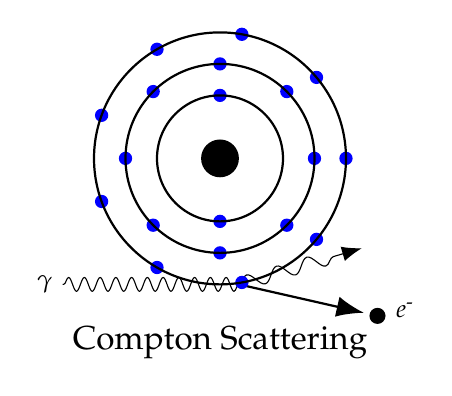
\begin{tikzpicture}[scale=.8]
            \draw[decorate, decoration=snake, segment length=2mm] (.3,-2) --
            (-2.5,-2) node[left] {\small$\gamma$};
            \draw[decorate, decoration=snake, segment length=4mm, -{Latex[scale=1.5]}, shorten >=-6] (.3,-2) -- (2.0,-1.5);
            \draw[thick, -{Latex[scale=1.5]}, shorten >=5] (.3,-2) -- (2.5,-2.5)
            node[draw, circle, fill=black, minimum size=5pt, inner sep=0pt] {}
            node[xshift=10pt, yshift=2pt] {\small$e^\text{-}$};
            \fill[black] (0,0) circle (0.3);
            \foreach \angle in {90, 270} {
                \fill[color=blue] (0,0) ++(\angle:1) circle (3pt);
            }
            \foreach \angle in {0, 45, 90, 135, 180, 225, 270, 315} {
                \fill[color=blue] (0,0) ++(\angle:1.5) circle (3pt);
            }
            \foreach \angle in {0, 40, 80, 120, 160, 200, 240, 280, 320} {
                \fill[color=blue] (0,0) ++(\angle:2cm) circle (3pt);
            }
            \foreach \radius in {1,1.5,2}
            {
                \draw[thick] (0,0) circle (\radius);
            }
            \node[below, font=\large] at (0,-2.5) {Compton Scattering};
        \end{tikzpicture}
    \end{minipage}
    % \begin{minipage}[t]{0.45\textwidth}
    %     \centering
    %     \begin{tikzpicture}[scale=.8]
    %         \draw[decorate, decoration=snake, segment length=2mm] (0,-.3) --
    %         (-2.5,-.3) node[left] {\small$\gamma$};
    %         \draw[thick, -{Latex[scale=1.5]}, shorten >=5] (0,-.3) -- (2.5,1)
    %         node[draw, circle, fill=black, minimum size=5pt, inner sep=0pt] {}
    %         node[xshift=10pt, yshift=2pt] {\small$e^\text{-}$};
    %         \draw[thick, -{Latex[scale=1.5]}, shorten >=5] (0,-.3) -- (2.5,-1.3)
    %         node[draw, circle, fill=black, minimum size=5pt, inner sep=0pt] {}
    %         node[xshift=10pt, yshift=2pt] {\small$e^\text{-}$};
    %         \fill[black] (0,0) circle (0.3);
    %         \foreach \angle in {90, 270} {
    %             \fill[color=blue] (0,0) ++(\angle:1) circle (3pt);
    %         }
    %         \foreach \angle in {0, 45, 90, 135, 180, 225, 270, 315} {
    %             \fill[color=blue] (0,0) ++(\angle:1.5) circle (3pt);
    %         }
    %         \foreach \angle in {0, 40, 80, 120, 160, 200, 240, 280, 320} {
    %             \fill[color=blue] (0,0) ++(\angle:2cm) circle (3pt);
    %         }
    %         \foreach \radius in {1,1.5,2}
    %         {
    %             \draw[thick] (0,0) circle (\radius);
    %         }
    %         \node[below, font=\large] at (0,-2.5) {Pair Production};
    %     \end{tikzpicture}
    % \end{minipage}
    \caption{Principles from photon interaction with matter similar to \cite[Chap. 7]{medicalImagingSystemsIntro2019:}}
    \label{fig:tungsten_atomic_model}
\end{figure}

\subsection{Free Path Length}

All mentioned interaction processes - the photoelectric effect, Compton
scattering and Rayleigh scattering - are probabilistic in nature. The according
attenuation coefficients $\mu$ characterizes the extend of the beam being
reduced by its according effect, when passing through the material, in \si{\square\centi\metre\per\gram}. For the
simulation of photons, the attenuation coefficients are dependend on the
according energy $E$ of the photon and the material at spherical location $x$ of
the photon. The coefficients are summarized in
Table~\ref{tab:attenuation_coefficients}.

\begin{table}[H]
    \centering
    \begin{tabular}{lcc}
        \toprule
        \textbf{Interaction Type} & \textbf{Attenuation Coefficient} \\
        \midrule
        Photoelectric Effect & $\mu_{\text{PE}}(x,E)$ \\
        Rayleigh Scattering & $\mu_{\text{RS}}(x,E)$ \\
        Compton Scattering & $\mu_{\text{CS}}(x,E)$ \\
        \bottomrule
    \end{tabular}
    \caption{Attenuation coefficients for different photon interaction mechanisms.}
    \label{tab:attenuation_coefficients}
\end{table}

The linear attenuation coefficient $\mu(x,E)$ is the sum of the individual
attenuation coefficients of the interaction coefficients:

$$\mu(x,E) = \mu_{\text{PE}}(x,E) + \mu_{\text{RS}}(x,E) +
\mu_{\text{CS}}(x,E)$$

When an X-ray photon eneters the phantom two main effects are considered:
\begin{itemize}
    \item \textbf{Attenuation:} The photon may be absorbed or Scattered.
    \item \textbf{No Interaction:} The photon may pass through the phantom
    without any interaction.
\end{itemize}

The \emph{free path length} $t$ of a photon describes the distance a photon takes to traverse through the phantom before it interacts with matter. Supposing the phantoms location is $x$ and the photon is traveling in the unit direction $\vec{v}$, as in \cite{qmcXray2023} the free path length $t$ follows the distribution given by:

$$t \sim \mu(x,E)\exp\bigg[-\int_{0}^{t}{\mu(x+s\cdot\vec{v})}\bigg]$$

\textcolor{red}{Check: nach dem paper müsste $\mu$ abhängig vom Endpunkt sein.}

The free path length $t$ is constraint by the maximum distance $c$ ($0\leq t\leq
c$) to the next exit point of the phantom along the ray with direction
$\vec{v}$. After leaving the phantom, we assume the photon is reaching the
detector or leaving the simulation domain.

The probability of the photon to leave the phantom unaltered is
described by the \emph{escape probability} $\mathcal{P}$ of a photon at a given
position $A$ with unit direction $\vec{v}$ and energy $E$ as in
\cite{qmcXray2023}:

$$\mathcal{P}(x, \vec{v}, E) = \exp \bigg[ -\int\limits_{0}^{c}{\mu(x+t\vec{v}, E)} dt \bigg],$$

\begin{figure}[H]
    \centering
    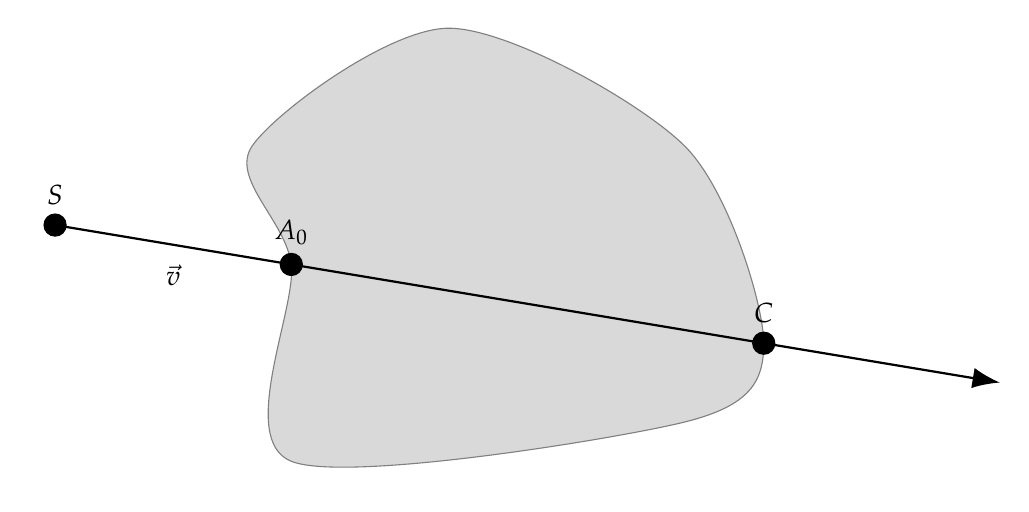
\begin{tikzpicture}[scale=1]
        \draw[color=gray, fill=gray!30] plot[smooth cycle] coordinates {(-2,0) (-2.5,1.5) (0,3) (3,1.5) (4,-1) (3,-2) (-2,-2.5)};
        \filldraw[fill=black] (-5,.5) circle (4pt) node[above, inner sep=7pt] {$S$};
        \node[below, inner sep=7pt] at (-3.5,.25) {$\vec{v}$};
        \draw[thick] (-5,.5) -- (-2,0);
        \filldraw[fill=black] (-2,0) circle (4pt) node[above, inner sep=7pt] {$A_0$};
        \draw[thick] (-2,0) -- (4,-1);
        \filldraw[fill=black] (4,-1) circle (4pt) node[above, inner sep=7pt] {$C$};
        \draw[thick, -{Latex[scale=1.5]}] (4,-1) -- (7,-1.5);

        % \node[above] at (-.5,.5) {$A_0$};
    \end{tikzpicture}
    \caption{Illustration of the entry and exit point of the ray of a photon without interaction.}
    \label{fig:exit_point}
\end{figure}

% \textcolor{green}{Todo: Image illustrating the entry and exit point of a ray without interaction.}


\subsection{Compton Scattering}
\label{sec:physicsComptonScattering}
\emph{Compton scattering} is the most dominant interaction mechanism for X-ray
photons in tissue \cite[Chap. 7]{medicalImagingSystemsIntro2019:}. It occurs
when a X-ray photon with considerably higher energy than the binding energy of an outer shell electron collides with this electron. This interaction
results in a transfer of energy and momentum. The electron is ejected from the atom, while the incoming photon is scattered at an
angle and its energy is reduced.

A portion of the incident photon energy is transferred to the electron, which
is referred to as the "recoil electron" or Compton electron. The interaction
produces a positive ion, the "recoil electron" and a scattered photon. If the deflection angle of the scattered photon is small, most of the energy is retained by the scattered photon. The deflection angle can vary from 0 to 180 degrees, depending on the energy transfer during the interaction.

For the distribution of the scattering angle $\theta$ of the scattered photons
in the differential cross section, we apply the formula derived by \emph{Klein
and Nishina} in 1928. This equation describes the distribution of the scattering
angle of X-ray photons in Compton scattering assuming the electron is initially
free and stationary, the relation between energy loss and photon deflection is
determined from conservation of momentum and energy between the photon and the
recoiling electron \cite{hubbell1969photon,klein1928scattering}.

\begin{equation}
    \label{eq:kleinNishina}
    \frac{d\sigma}{d\Omega} = \frac{1}{2} r_e^2 \frac{1}{(1 + k(1 - \cos \theta))^2} \left( 1 + \cos^2 \theta + \frac{k^2 (1 - \cos \theta)^2}{1+ k(1 - \cos \theta)} \right)
\end{equation}

where $k=\frac{e}{mc^2} \approx \frac{E}{0.511}$ with $mc^2$ being the rest mass
energy of the electron, $E$ being the energy of the incident photon and $r_e$
being the classical electron radius.

For sampling from the distribution of the scattering angle we cannot apply the
same procedure as for the photon energy in Section~\ref{sec:photon_energy},
since the Klein-Nishina formula is not a cumulative distribution function (CDF).
Instead the method of \emph{rejection sampling} is used. 

Rejection sampling is a technique to generate samples from a target distribution
by using an envelope distribution that is easy to sample from. The envelope
distribution is an upper bound to the original distribution. The basic idea is
to sample from this proposal distribution and accept or reject the samples based
on a criterion that relates the envelope distribution to the target distribution
from Klein-Nishina \cite[Chap. 4]{muller2012monte}.

In the context of the distribution of Klein-Nishina, the convergence behavior for $E\to\infty$ and $k\to\infty$ consequently is:

\begin{equation}
    f(k,x) \in \mathcal{O} (\frac{1}{k(1-x)})
\end{equation}

A suitable envelope distribution is of the form
\begin{equation*}
    h(k,x) = \frac{1}{k(1-x)}
\end{equation*}

with the given conditions
\begin{align*}
    f(k,1) &= h(k,1) = 2 \\
    f(k,-1) &= h(k,-1) = \zeta(k) \\
    \zeta(k) &= \frac{2(2k^2 + 2k + 1)}{(2k + 1)^3}
\end{align*}
By a straightforward calculation, this leads to the following values\cite{ozmutlu1992sampling}:
\begin{align*}
    a(k) = 2(b(k)-1) \\
    b(k) = \frac{1+\frac{\zeta(k)}{2}}{1-\frac{\zeta(k)}{2}}
\end{align*}

Now by using the rejection sampling method, $x=\cos\theta$ is sampled from the distribution $h$ by generating a uniform random variable $r \sim \mathcal{U}(0,1)$ and calculating the value $x$ as follows:
\begin{equation}
    x = b(k)- (b(k)-1) \left(\frac{\zeta}{2}\right)^r
\end{equation}

We will accept this value if $\frac{f(k,x)}{h(k,x)} \geq u_1$, where $u_1$ denotes the random input variable. To derive an exact direction of the scattered photon, we need to further sample an azimuthal angle $\phi$, which is done by the second random input variable:
\begin{equation}
    \label{eq:azimuthal_angle}
    \phi = 2\pi u_2
\end{equation}

Once the scattering angle $\theta$ is sampled, the energy of the scattered
photon $E'$ can be calculated using the Compton formula:

\begin{equation}
    \label{eq:compton_energy}
    E' = \frac{E}{1 + \frac{E}{m_e c^2} (1 - \cos \theta)}
\end{equation}

\subsection{Rayleigh Scattering}
\emph{Rayleigh scattering} is a type of elastic scattering that occurs at low X-ray energies \cite[Chap. 7]{medicalImagingSystemsIntro2019:}. The incident photon interacts with several electrons that are
usually bound in the outer shells of the atom. In this process, the low energy photon is not ejected, but rather the electrons and in turn thw whole atom is
set to vibration with respect to the incident photon’s wavelength. The vibrating photon transfers its excess energy to an electromagnetic photon with the same wavelength but probably a different direction than the incident photon. The majority of these scattered photons are emitted in a forward direction. This interaction does not result in the ejection of electrons from the atom and no ionization occurs as no energy is converted into kinetic energy.

Although Rayleigh scattering is taking place in the X-ray tube, it can be 
excluded from the linear attenuation coefficient, as it does not contribute to
the attenuation of the X-ray beam in the same way as Compton scattering or
photoelectric absorption. As described in \cite{poludniowski2022calculating}, the exclusion of Rayleigh scattering from the linear attenuation coefficient is based on the assumption that the characteristic radiation emitted by the target is isotropic, meaning it is emitted uniformly in all directions. As the X-ray is not attenuated by Rayleigh scattering, it is a common assumption to exclude Rayleigh scattering from the attenuation coefficient.

%!TEX root = ../main.tex
\chapter{The Simulation Algorithm}
\label{Chapter5}

This chapter presents the algorithm used for X-ray image simulation. It
incorporates elements of \emph{Forced Detection} as introduced in \cite{fd2001},
in order to accelerate convergence.

Unlike standard Monte Carlo simulations, where a random variable determines
whether a photon escapes the phantom or undergoes another scattering event, the
forced detection approach employed, calculates the probability of escaping the
phantom at each interaction point and reflects this distribution in accordingly
updated photon intensities for the case of escaping the phantom and the case of
scattering. Instead of probabilistically terminating the photon trajectory, the
algorithm tracks it through a predefined number of scattering events $N$. At
each interaction, the remaining intensity is updated to reflect both the
probability of Compton scattering and the conditional escape probability. This
ensures that both potential outcomes—escape or continued scattering—are
implicitly accounted for in the evolving photon intensity. As a result, the
simulation maintains physical accuracy while achieving a significant reduction
in variance.

When a photon eventually escapes the phantom, it contributes to the
corresponding detector pixel, weighted by its current intensity, photon energy,
and escape probability. Conversely, the distance to the next interaction is
sampled based on the probability of not escaping the phantom. Further
implementation details are discussed in Section~\ref{sec:algorithmOverview}.

This variance reduction strategy enables the simulation to converge more rapidly
toward high-resolution images with suppressed noise and well-preserved
structural detail.


%-------------------------------------------------------------------------------
%	SECTION 1
\section{Algorithm overview}
\label{sec:algorithmOverview}
%-------------------------------------------------------------------------------

The algorithm begins by initializing a set of photons, each assigned an initial
energy $E_0$, sampled from the X-ray tube spectrum and an initial direction
$\vec{\omega}_0$ sampled uniformly within a cone centered around the principal
beam axis. A total of three random variables are drawn for each photon to
determine its energy and direction.

Given a fixed source position $A$ representing the location of the X-ray tube,
each photon's initial origin is placed within a voxel grid composed of cubic
voxels that define the geometry of the scene. Each voxel encodes an integer
value identifying a specific material or tissue type. Furthermore, each photon
is initialized with an intensity of $W_0=1$, which is iteratively updated
throughout the simulation to account for attenuation and scattering processes.

\begin{figure}[H]
    \centering
    \tdplotsetmaincoords{70}{120} % view angle
    \begin{tikzpicture}[tdplot_main_coords, scale=.7]

    % Grid size
    \def\N{3}

    % Draw voxels
    \foreach \x in {0,...,2} {
        \foreach \y in {0,...,2} {
            \foreach \z in {0,...,2} {
                \draw[gray, thick] (\x,\y,\z) -- ++(1,0,0) -- ++(0,1,0) -- ++(-1,0,0) -- cycle; % bottom face
                \draw[gray, thick] (\x,\y,\z) -- ++(0,0,1); % vertical lines from bottom
                \draw[gray, thick] (\x+1,\y,\z) -- ++(0,0,1);
                \draw[gray, thick] (\x,\y+1,\z) -- ++(0,0,1);
                \draw[gray, thick] (\x+1,\y+1,\z) -- ++(0,0,1);
                \draw[gray, thick] (\x,\y,\z+1) -- ++(1,0,0) -- ++(0,1,0) -- ++(-1,0,0) -- cycle; % top face
            }
        }
    }

    % Optional axis labels
    \draw[->, thick] (0,0,0) -- (3.5,0,0) node[anchor=north east]{$x$};
    \draw[->, thick] (0,0,0) -- (0,3.5,0) node[anchor=north west]{$y$};
    \draw[->, thick] (0,0,0) -- (0,0,3.5) node[anchor=south]{$z$};

    \end{tikzpicture}
\end{figure}

Then an algorithm is applied to traverse the photon through the voxel grid until
it reaches the first material which is not air. This is done with a ray
traversal algorithm. Once the phantom at a point $A_0$ is reached, the photon
transport is simulated by the physical laws described in Chapter~\ref{Chapter6}.

Hereby, as in all other scatter points within the phantom, the free \emph{free
path length} $t_i$ is sampled from the exponential distribution based on
\emph{Beer-Lambert's law} (Eq.~\ref{eq:lambert_beer_law}) and the \emph{total
attenuation coefficient} $\mu(A_i, E_i)$ accordingly. $A_i$ hereby denotes the
current position and $E_i$ the current energy. First, the \emph{escape
probability} depending on the current position $A_i$ and the unit direction
$\vec{\omega}_i$ and the energy $E_i$ is computed. The escape probability in
Equation~\ref{eq:escapeProbability} is the probability of the photon escaping
the phantom at the current position $A_i$ without being further scattered.

\begin{equation}
    \label{eq:escapeProbability}
    p(A_i, \omega_i, E_i) = \exp\bigg(-\int\limits_{\overrightarrow{A_iC_i}} \mu(x, E_i) dx\bigg)
\end{equation}

Hereby $C_i$ denotes the exit point of the phantom in the direction of the photon $\vec{\omega}_i$. The escape probability is used to determine the intensity of the photon without the $(i+1)$-th scatter event.

Using one random variable $u_{3i+1}$, the free path length is sampled. Hereby both cases are being considered:

\begin{enumerate}
    \item \textbf{Photon escapes the phantom without further scattering:}\\
        This happens with the portion matching the escape probability $p(A_i,
        \omega_i, E_i)$. Accordingly 
        \begin{equation}
            W^{\text{escape}}_{i+1} = W_i \cdot p(A_i, \omega_i, E_i)
        \end{equation}
        The photon contributes to the detector signal in direction
        $\vec{\omega}_i$ with a final intensity of $E_i \cdot
        W^{\text{escape}}_{i+1}$. In case $i=0$, this intensity is accounted as
        priamry intensity.

    \item \textbf{Photon does not escape the phantom and scatters:}\\
        This happens with the portion matching the inverse of the escape
        probability $1 - p(A_i, \omega_i, E_i)$. Accordingly, the free path
        length is sampled from the exponential distribution by solving
        Equation~\ref{eq:freePathLength} for $t_i$:
        \begin{equation}
            \label{eq:freePathLength}
            \exp\bigg(-\int\limits_0^{t_i} \mu(A_{i} + s \cdot \vec{\omega}_
            {i}, E_{i}) ds\bigg) = u_{3i+4}
        \end{equation}
        Accordingly, the next scatter point is being computed as:
        \begin{equation}
            A_{i+1} = A_i + t_i \cdot \vec{\omega}_i
        \end{equation}
        The photon intensity is then updated with:
        \begin{equation}
            W_{i+1} = W_i \cdot (1 - p(A_i, \omega_i, E_i)) \cdot \frac{\mu_
            {\text{CS}}(A_{i+1}, E_i)}{\mu(A_{i+1}, E_i)}
        \end{equation}
\end{enumerate}


In the next step, the photon energy and opening angle after the Compton scatter
event is sampled with a second random variable $u_{3i+2}$. A thrid variable is
used to apply a azimuthal rotation around the direction of the photon
$\vec{\omega}_i$ to sample the new direction $\vec{\omega}_{i+1}$ of the photon
after the scatter event.

This process is repeated according to the maximum scatter order $N$.

\textcolor{red}{TODO: what happens with the leftover intensity? It is forwarded without any further scattering!}

%-------------------------------------------------------------------------------
%	SECTION 2
\section{Sub-Algorithms}
\label{sec:subAlgorithms}
%-------------------------------------------------------------------------------

To model the relevant physical processes in a structured manner, the main
simulation is decomposed into several sub-algorithms. This section describes the
purpose and implementation of each sub-algorithm in detail.

\subsection{Photon Generation}
For the photon generation step, two fundamental properties are sampled for each
photon:

\begin{itemize}
    \item \emph{Photon energy}, sampled using a single random variable from the
    X-ray spectrum.
    \item \emph{Photon direction}, sampled using two random variables uniformly
    within a cone defined by the beam axis $\vec{d}$ and opening angle $\alpha$.
\end{itemize}

\subsubsection{Photon Energy Sampling}

The photon energy is sampled from the X-ray tube spectrum, which is represented
as a discrete set of energy values with corresponding fluence values. The
spectrum was generated using \emph{Spekpy}~\cite{spekpy,poludniowski2021spekpy},
based on an X-ray tube configured with the parameters listed in
Table~\ref{tab:xray_params}.

\begin{table}[H]
    \centering
    \begin{tabular}{ll}
        \toprule
        \textbf{Parameter}      & \textbf{Value} \\
        \midrule
        Tube voltage            & 120\,kV \\
        Anode material          & Tungsten \\
        Filtration              & 0.4\,\si{\milli\meter} Tin (Sn),
        0.1\,\si{\milli\meter} Copper (Cu) \\
        Target angle            & 12.5\textdegree \\
        \bottomrule
    \end{tabular}
    \caption{Parameters used to generate the X-ray spectrum with \emph{Spekpy}.}
    \label{tab:xray_params}
\end{table}

Photon energies are sampled using inverse transform sampling. The algorithm
normalizes the fluence values to obtain a probability density function (PDF),
computes the corresponding cumulative distribution function (CDF) and uses a
uniformly distributed random variable to select an energy according to the CDF.

\begin{algorithm}[H]
\caption{Photon Energy Sampling from Spectrum}
\label{alg:photonEnergySampling}
\begin{algorithmic}[1]
\Require Array of energies $E = [E_1, E_2, \dots, E_n]$ 
\Require Corresponding fluence values $\Phi = [\phi_1, \phi_2, \dots, \phi_n]$ 
\Require Number of samples $N$ 
\Require Random variable $u \sim \mathcal{U}(0, 1)$ \Ensure Sampled photon
energies $S = [s_1, s_2, \dots, s_N]$

\LineComment{Normalize fluence values:} \State $$T \gets \sum_{i=1}^{n} \phi_i$$
\State $$\text{PDF}[i] \gets \frac{\phi_i}{T}$$

\LineComment{Compute cumulative distribution function:} 
\State $$\text{CDF}[1] \gets \text{PDF}[1]$$ 
\For{$i = 2$ to $n$} 
\State $\text{CDF}[i] \gets \text{CDF}[i-1] + \text{PDF}[i]$ 
\EndFor

\LineComment{Note: $PDF[i]>0$ in the spectrum, therefore $\text{CDF}$ is
strictly increasing.}

\State Create interpolating function $\text{ InverseCDF}(u)$ from
$(\text{CDF}[i], E[i])$

\State \Return $\text{InverseCDF}(u)$

\end{algorithmic}
\end{algorithm}

\subsubsection{Photon Direction Sampling}

The direction of each photon is sampled uniformly within a cone defined by the
beam axis $\vec{d}$ and opening angle $\alpha$. This requires two independent
random variables $u_1, u_2 \sim \mathcal{U}(0, 1)$.

Algorithm~\ref{alg:uniformDirectionSampling}, adapted
from~\cite{venkatapathi2021n}, generates a random unit vector $\vec{v}$
uniformly distributed within a cone of half-angle $\alpha$ around the direction
$\vec{d}$:

\begin{enumerate}
    \item \textbf{Sampling the polar angle $\theta$}:\\
    Draw $u_1 \sim \mathcal{U}(0,1)$ and compute
    \[
        \theta = \arccos\left(1 - u_1 (1 - \cos \alpha)\right).
    \]
    This corresponds to inverse transform sampling such that $\cos\theta$ is
    uniformly distributed on $[\cos\alpha, 1]$, resulting in uniform sampling
    over the spherical cap.

    \item \textbf{Sampling the azimuthal angle $\phi$}:\\
    Draw $u_2 \sim \mathcal{U}(0,1)$ and compute
    \[
        \phi = 2\pi u_2,
    \]
    ensuring a uniform distribution around the cone axis.

    \item \textbf{Constructing the local direction vector}:\\
    In a local spherical coordinate system with the cone axis aligned along the
    $z$-axis, the sampled unit vector is
    \[
        \vec{v}_{\text{local}} =
        \begin{pmatrix}
            \sin\theta \cos\phi \\
            \sin\theta \sin\phi \\
            \cos\theta
        \end{pmatrix}.
    \]

    \item \textbf{Rotation into global coordinates}:\\
    To align the cone axis from the local $z$-axis to an arbitrary unit vector
    $\vec{d}$, an orthonormal basis $(\vec{u}, \vec{v}, \vec{d})$ is constructed
    via the Gram–Schmidt process:
    \begin{itemize}
        \item Choose a helper vector $\vec{a} = (0,0,1)$ if $|d_3| < 0.999$,
        otherwise $\vec{a} = (1,0,0)$.
        \item Compute $\vec{u} = \frac{\vec{a} \times \vec{d}}{\|\vec{a} \times
        \vec{d}\|}$.
        \item Set $\vec{v} = \vec{d} \times \vec{u}$ to complete a right-handed
        orthonormal basis.
    \end{itemize}
    Finally, rotate $\vec{v}_{\text{local}}$ into global coordinates via the
    transformation
    \[
        \vec{v}_{\text{global}} = (\vec{v}_{\text{local}})_x \vec{u} + (\vec{v}_{\text{local}})_y \vec{v} + (\vec{v}_{\text{local}})_z \vec{d}.
    \]
\end{enumerate}


\begin{algorithm}[H]
\caption{Uniform Direction Sampling Within a Cone}
\label{alg:uniformDirectionSampling}
\begin{algorithmic}[1]
\Require Cone angle $\alpha$
\Require Unit beam direction vector $\vec{d} = (d_1, d_2, d_3)$
\Require Random variables $u_1, u_2 \sim \mathcal{U}(0,1)$
\Ensure Sampled direction vector $\vec{v}$ uniformly within cone around
$\vec{d}$

\LineComment{Calculate angles according to samples}

\State $\theta \gets \arccos(1 - u_1 (1 - \cos \alpha))$ \Comment{Polar angle}
\State $\phi \gets 2\pi u_2$ \Comment{Azimuthal angle}

\LineComment{Calculate local direction vector in spherical coordinates}

\State $$\vec{v}_{\text{local}} \gets 
\begin{pmatrix}
\sin\theta \cos\phi \\
\sin\theta \sin\phi \\
\cos\theta \end{pmatrix}$$

\LineComment{Orthonormal basis construction (Gram-Schmidt)}
\If{$|d_3| < 0.999$}
    \State $\vec{a} \gets (0, 0, 1)$
\Else
    \State $\vec{a} \gets (1, 0, 0)$
\EndIf
\State $\vec{u} \gets \frac{\vec{a} \times \vec{d}}{\|\vec{a} \times \vec{d}\|}$ \Comment{Orthogonal vector}
\State $\vec{v} \gets \vec{d} \times \vec{u}$ \Comment{Complete right-handed basis}

\LineComment{Rotate local vector into global coordinates}
\State $\vec{v}_{\text{global}} \gets \vec{u} (\vec{v}_{\text{local}})_x + \vec{v} (\vec{v}_{\text{local}})_y + \vec{d} (\vec{v}_{\text{local}})_z$

\State \Return $\vec{v}_{\text{global}}$

\end{algorithmic}
\end{algorithm}


\subsection{Ray Traversal}
\label{sec:rayTraversal}

The ray traversal algorithm is responsible for simulating the propagation of a
photon through the voxel grid. It is used to forward the photon until it reaches
the first chemical compound, which is not air (or is air). It is also
used to simulate the photon transport within the phantom until it reaches the
exit point of the phantom.

The Input values of the algorithm are:
\begin{itemize}
    \item The voxel grid $materialGrid$ representing the geometry of the scene.
    \item The initial position of the photon $A$.
    \item The (unit) direction of the photon $\vec{\omega}$.
\end{itemize}

The algorithm traverses the photon through the voxel grid, voxel by voxel while checking the material of the next voxel and iterrupts in case the next voxel is not air (or is air).

The return values of the algorithm are:
\begin{itemize}
    \item The coordinates of the final postion: $C$
    \item An array of all crossed voxel indices: $crossedVoxels$
    \item An array of all crossed voxel materials: $crossedMaterials$
    \item An array of al entry points of each crossed voxel: $entryPoints$
    \item An array of the distances traveres in each voxel: $distances$
    \item A boolean mask indicating whether the photon exited the grid:
    $exitGrid$
\end{itemize}

The sequence of the algorithm can be summarized as follows:
\begin{enumerate}[label=\Roman*.]
    \item Initialize empty arrays for $crossedVoxels$, $crossedMaterials$, $entryPoints$ and $distances$.
    \item Convert the photon position $A$ into voxel coordinates $pos$.
    \item Determine the indices of the next voxel $voxelIdx$ based on the
    $pos$ and the direction $\vec{\omega}$.
    \item Set $exitGrid$ to false.
    \item \textbf{If} the $voxelIdx$ of the next voxel is out of bounds, set $exitGrid$ to true and exit the algorithm.
    \item Determine $material$ of the next $voxelIdx$
    \item \textbf{If} the $material$ is not air, exit the algorithm.
    \item \textbf{While} $material$ is air:
        \begin{enumerate}[label=\arabic*.]
            \item Append $voxelIdx$ to $crossedVoxels$.
            \item Append $material$ to $crossedMaterials$.
            \item Append $pos$ to $entryPoints$.
            \item Determine $maxDist$ to the next voxel boundary.
            \item Append $maxDist$ to $distances$.
            \item Update $pos$ by adding $\vec{\omega} \cdot maxDist$.
            \item Determine $voxelIdx$ of the next voxel based on the updated $pos$.
            \item \textbf{If} the $voxelIdx$ is out of bounds, set $exitGrid$ to true and exit the algorithm.
            \item Determine $material$ of the next $voxelIdx$.
        \end{enumerate}
\end{enumerate}

When the algorithm finishes, the final Position $C$ is set to the last value of
$position$.

To use this agorithm for travering the photons through air until they reach the phantom and to traverse the photons through the phantom until they reach the exit point of the phantom, the algorithm is called with the boolean value $throughAir$. In case $throughAir=true$, the algorithm will traverse the photons through air until they reach the first material which is not air. In case $throughAir=false$, the algorithm will traverse the photons through the phantom until they reach the exit point of the phantom.

Therefore we define a short helper function in
Algorithm~\ref{alg:rayTraversalHelper} beforehand, which generates the specific
expression depending on the boolean value of $throughAir$.

\begin{algorithm}[H]
\caption{Ray Traversal Helper Function}
\label{alg:rayTraversalHelper}
\begin{algorithmic}[1]
\Require Boolean $throughAir$
\Require $material$
\Ensure Boolean value
\If {$throughAir$}
    \State \Return $material = \text{air}$
\Else
    \State \Return $material \neq \text{air}$
\EndIf
\end{algorithmic}
\end{algorithm}

Algorithm~\ref{alg:rayTraversal} implements the process of ray traversing
through the voxel grid in detail.

\begin{algorithm}[H]
    \caption{Ray Traversal Algorithm}
    \label{alg:rayTraversal}
    \begin{algorithmic}[1]
        \Require Boolean $throughAir$
        \Require Material grid $materialGrid \in \mathbb{Z}^{X \times Y \times
        Z}$, voxel size $s \in \mathbb{R}^+$
        \Require Initial pos $A \in \mathbb{R}^3$, direction $\vec{\omega} \in
        \mathbb{R}^3$
        \Ensure Final pos $C \in \mathbb{R}^3$
        \Ensure Arrays $crossedVoxels, crossedMaterials, entryPoints, distances$
        \Ensure Boolean $exitGrid$ indicating whether the photon exited the grid
        \State $pos \gets O / s$
        \State $exitGrid \gets \text{false}$
        \State $currentVoxelIdx \gets \lfloor pos \rfloor$
        \State $negDir$ $\gets \vec{\omega} < 0$
        \State $onB \gets (pos = \lfloor currentVoxelIdx \rfloor)$
        \State $nextVoxelIdx \gets currentVoxelIdx$
        \State $nextVoxelIdx[negDir \land onB] \gets nextVoxelIdx[negDir
        \land onB] - 1$
        \If{any($nextVoxelIdx < 0$) or any($nextVoxelIdx \geq
        \text{shape}(materialGrid)$)}
            \State $exitGrid \gets \text{true}$
            \State $C \gets pos$
            \State \Return $C, crossedVoxels, crossedMaterials,entryPoints, 
            distances, exitGrid$
        \EndIf
        \State $material \gets materialGrid[nextVoxelIdx]$
        \While{Algorithm~\ref{alg:rayTraversalHelper}(throughAir, material)}
            \State $crossedVoxels.\text{append}(nextVoxelIdx)$
            \State $crossedMaterials.\text{append}(material)$
            \State $entryPoints.\text{append}(pos)$
            \State $fracPos \gets pos - \lfloor pos \rfloor$
            \State $maxDist \gets [\infty, \infty, \infty]$
            \State $negDir$ $\gets \vec{\omega} < 0$
            \State $posDir$ $\gets \vec{\omega} > 0$
            \State $onB \gets (pos = \lfloor currentVoxelIdx \rfloor)$
            \State $maxDist[negDir \land onB] \gets -1 / \vec{\omega}[negDir
            \land onB]$
            \State $maxDist[negDir \land \neg onB] \gets 
            -fracPos[negDir \land \neg onB] / \vec{\omega}
            [negDir \land \neg onB]$
            \State $maxDist[posDir] \gets (1 - fracPos[posDir]) / \vec{\omega}
            [posDir]$
            \State $distance = \min(maxDist)$
            \State $distances.\text{append}(maxDist)$
            \State $pos \gets pos + \vec{\omega} \cdot distance$
            \State $currentVoxelIdx \gets \lfloor pos \rfloor$
            \State $nextVoxelIdx \gets currentVoxelIdx$
            \State $nextVoxelIdx[negDir \land onB] \gets nextVoxelIdx[negDir
            \land onB] - 1$
            \If{any($nextVoxelIdx < 0$) or any($nextVoxelIdx \geq
            \text{shape}(materialGrid)$)}
                \State $exitGrid \gets \text{true}$
                \State $C \gets pos$
                \State \Return $C, crossedVoxels, crossedMaterials, entryPoints,
                distances, exitGrid$
            \EndIf
            \State $material \gets materialGrid[nextVoxelIdx]$
        \EndWhile
        \State $C \gets pos$
        \State \Return $C, crossedVoxels, crossedMaterials, entryPoints, distances, exitGrid$

    \end{algorithmic}
\end{algorithm}

\subsection{Forced Detection}

The forced detection algorithm is responsible to apply one iteration of the
forced detection process to a photon within the phantom. Hereby the algorithm
accounts:

\begin{itemize}
    \item The voxel grid $materialGrid$ representing the geometry of the scene.
    \item The voxel grid $totalAttenuationGrid$ representing the attenuation coefficients of the materials in the voxel grid $materialGrid$.
    \item The voxel grid $comptonAttenuationGrid$ representing the Compton scattering coefficients of the materials in the voxel grid $materialGrid$.
    \item The voxel grid $absorptionGrid$ representing the absorption coefficients of the materials in the voxel grid $materialGrid$.
    \item The initial position of the photon $A_i$.
    \item The (unit) direction of the photon $\vec{\omega}_i$.
    \item The initial energy of the photon $E_i$.
    \item The initial intensity of the photon $W_i$.
    \item A random variable $u \sim \mathcal{U}(0, 1)$ to sample the free path length.
    \item The voxel size $s$.
\end{itemize}

The algorithm then applies the ray traversal algorithm
(Algorithm~\ref{alg:rayTraversal}) to traverse the photon through the phantom
until it reaches the exit point of the phantom $C_i$. Obtaining the exit point
$C_i$, the arrays of $crossedVoxels$ and $distances$, now the attenuation
coefficients of the materials along the ray can be extracted from the voxel
grids for the crossed voxels:

\begin{align*}
    \label{eq:gatAttenuation}
    totalAttenuationCoefficients &= totalAttenuationGrid[crossedVoxels] \\
    comptonScatteringCoefficients &= comptonAttenuationGrid[crossedVoxels]
\end{align*}

With the following helper algorithm (Algorithm~\ref{alg:partialProductSum}), the $escapeProbability$ is computed. Further the last distance index $k$ and last interpolation factor $f$ are returned, to solve Equation~\ref{eq:freePathLength} for the free path length $t_i$, which can then be simply computed by:

\begin{equation}
    t_i = \sum_{j=0}^{k-1} distances[j] + f
\end{equation}

Now the next scatter point $A_{i+1}=A_i+t_i\cdot s \cdot\vec{\omega}_i$ can be
determined and the new intensities together with the exit point $C_i$ can be
computed:

\begin{align*}
    voxelIdx &= \lfloor A_{i+1} / s \rfloor \\
    W_{i+1} &= W_i \cdot (1 - escapeProbability) \cdot \frac
    {comptonAttenuationGrid[voxelIdx]}{totalAttenuationCoefficients[voxelIdx]} 
    \\
    W^{\text{escape}}_{i+1} &= W_i \cdot escapeProbability
\end{align*}

And accordingly the forced detection algorithm returns the following values:
\begin{itemize}
    \item The new position of the photon $A_{i+1}$.
    \item The new intensity of the photon after the scatter event $W_{i+1}$.
    \item The intensity of the photon for the case of escaping the phantom $W^{\text{escape}}_{i+1}$.
    \item The exit point of the phantom $C_i$.
    \item The Compton scattering coefficient $\mu_{\text{CS}}$ at the scatter
    point $A_{i+1}$.
\end{itemize}

\begin{algorithm}[!tp]
\caption{Partial Product Sum for Free Path Sampling in Forced Detection}
\label{alg:partialProductSum}
\begin{algorithmic}[1]
\Require Arrays $distances, totalAttenuationCoefficients \in \mathbb{R}^n$, weight $u \in [0, 1]$
\Ensure Last distance index $k$, last interpolation factor $f$,
$escapeProbability$

\State $S_\text{total} \gets 0$
\State Initialize array $P[0\ldots n-1]$

\For{$i \gets 0$ to $n-1$}
    \State $P[i] \gets distances[i] \cdot totalAttenuationCoefficients[i]$
    \State $S_\text{total} \gets S_\text{total} + P[i]$
\EndFor

\State $T \gets u \cdot S_\text{total}$
\State $S \gets 0$

\For{$i \gets 0$ to $n-1$}
    \If{$S + P[i] > T$}
        \State $f \gets \frac{T - S}{totalAttenuationCoefficients[i]}$
        \State \textbf{return} $(i, f, S_\text{total})$
    \EndIf
    \State $S \gets S + P[i]$
\EndFor

\State \textbf{return} $(n, 1.0, S_\text{total})$ \Comment{u = 1.0 or exact fit}
\end{algorithmic}
\end{algorithm}


\begin{algorithm}[H]
\caption{Forced Detection Algorithm}
\label{alg:forcedDetection}
\begin{algorithmic}[1]
\Require Material grid $materialGrid \in \mathbb{Z}^{X \times Y \times Z}$
\Require Total attenuation grid $totalAttenuationGrid \in \mathbb{R}^{X \times 
Y \times Z}$
\Require Compton scattering grid $comptonAttenuationGrid \in \mathbb{R}^{X 
\times Y \times Z}$
\Require Absorption grid $absorptionGrid \in \mathbb{R}^{X \times Y \times Z}$
\Require Initial position $A_i \in \mathbb{R}^3$
\Require Unit direction $\vec{\omega}_i \in \mathbb{R}^3$
\Require Initial energy $E_i \in \mathbb{R}^+$
\Require Initial intensity $W_i \in \mathbb{R}^+$
\Require Random variable $u \sim \mathcal{U}(0, 1)$
\Require Voxel size $s \in \mathbb{R}^+$
\Ensure New position $A_{i+1} \in \mathbb{R}^3$
\Ensure New intensity $W_{i+1} \in \mathbb{R}^+$
\Ensure Escape intensity $W^{\text{escape}}_{i+1} \in \mathbb{R}^+$
\Ensure Exit point $C_i \in \mathbb{R}^3$
\Ensure Compton Attenuation coefficient $\mu_{\text{CS}}$
\State $C_i, crossedVoxels, crossedMaterials, entryPoints, distances, exitGrid
\gets \text{Algorithm~\ref{alg:rayTraversal}}(throughAir = true, materialGrid,
s, A_i)$
\If{exitGrid}
    \State \Return $(C_i, W_i, 0, C_i)$ \Comment{Photon escaped the phantom}
\EndIf
\State $totalAttenuationCoefficients \gets totalAttenuationGrid[crossedVoxels]$
\State $comptonScatteringCoefficients \gets comptonAttenuationGrid
[crossedVoxels]$
\State $absorptionCoefficients \gets absorptionGrid[crossedVoxels]$
\State $k, f, escapeProbability \gets \text{Algorithm~\ref{alg:partialProductSum}}
(distances, totalAttenuationCoefficients, u)$
\State $escapeProbability \gets \frac{escapeProbability}{\sum_{j=0}^{k-1} distances
[j] \cdot totalAttenuationCoefficients[j]}$
\State $t_i \gets \sum_{j=0}^{k-1} distances[j] + f$
\State $A_{i+1} \gets A_i + t_i \cdot s \cdot \vec{\omega}_i$
\State $voxelIdx \gets \lfloor A_{i+1} / s \rfloor$
\State $\mu_{\text{CS}} \gets comptonScatteringCoefficients[voxelIdx]$
\State $W_{i+1} \gets W_i \cdot (1 - escapeProbability) \cdot
\frac{\mu_{\text{CS}}}{totalAttenuationCoefficients [voxelIdx]}$
\State $W^{\text{escape}}_{i+1} \gets W_i \cdot escapeProbability$
\State \Return $(A_{i+1}, W_{i+1}, W^{\text{escape}}_{i+1}, C_i,
\mu_{\text{CS}})$
\end{algorithmic}
\end{algorithm}


\subsection{Photon Exit Point Determination}

To determine the exit point of the photon in the world after exiting the phantom, a more efficient algorithm than the ray traversal algorithm from Section~\ref{sec:rayTraversal} is used can be applied. This algorithm yields the exit point of the phantom which is used to determin the detector pixel the photon contributes to.

The algorithm is initialized with the following parameters:
\begin{itemize}
    \item The voxel grid shape $(N_x,N_y,N_z)$ of the $materialGrid$
    representing the
    geometry of the scene.
    \item The initial position of the photon $C^{\text{phantom}}$.
    \item The (unit) direction of the photon $\vec{\omega}$.
    \item The voxel size $s$.
\end{itemize}

The algorithm then computes the point where the photon exits the voxel grid
efficiently and returns the exit point $C^{\text{grid}}$ and the according
Coordinates $C^{\text{gridCoords}}$. The algorithm is implemented as follows:

\begin{algorithm}[H]
\caption{Compute Exit Point of Ray from Voxel Grid}
\label{alg:exitPointComputation}
\begin{algorithmic}[1]
\Require Ray origin $C^{\text{phantom}} \in \mathbb{R}^3$, direction $\vec{\omega} \in \mathbb{R}^3$
\Require Grid shape $(N_x, N_y, N_z)$, voxel size $s \in \mathbb{R}^+$
\Ensure Exit point $C^\text{grid}$, $C^{\text{gridCoords}}$
\State $C^{\text{phantomCoords}} \gets C^{\text{phantom}} / s$ \Comment{Convert to voxel coordinates}
\State $x_{\min} \gets 0$, $x_{\max} \gets N_x$
\State $y_{\min} \gets 0$, $y_{\max} \gets N_y$
\State $z_{\min} \gets 0$, $z_{\max} \gets N_z$

\For{axis in \{x, y, z\}}
    \State $o \gets C^{\text{phantomCoords}}_\text{axis}$
    \State $d \gets \vec{\omega}_\text{axis}$

    \If{$d > 0$}
        \State $t^{(\text{axis})} \gets \frac{x_{\max} - o}{d}$
    \ElsIf{$d < 0$}
        \State $t^{(\text{axis})} \gets \frac{x_{\min} - o}{d}$
    \ElsIf{$d = 0$}
        \State $t^{(\text{axis})} \gets -\infty$
    \EndIf
\EndFor
\State $t_\text{exit} \gets \min(t^{(x)}, t^{(y)}, t^{(z)})$ \Comment{Exit time}
\State $C^{\text{gridCoords}} \gets C^{\text{phantomCoords}} + t_\text{exit} \cdot \vec{\omega}$
\State $C^{\text{grid}} \gets C^{\text{gridCoords}} \cdot s \cdot \vec{\omega}$ 
\State \textbf{return} $C^{\text{grid}}$, $C^{\text{gridCoords}}$
\end{algorithmic}
\end{algorithm}


\subsection{Compton Scattering}

The Compton scattering algorithm is responsible for simulating the physical process for the event of Compton scattering. Based on the Klein-Nishina formula (Equation~\ref{eq:kleinNishina}) and the rejection sampling method from Section~\ref{sec:physicsComptonScattering}, the algorithm samples the scatter angle and computes the new photon energy and direction after the scattering event.

The algorithm initializes with the following parameters:

\begin{itemize}
    \item The initial energy of the photon $E_i$.
    \item The (unit) direction of the photon $\vec{\omega}_i$.
    \item Two random variables $u_1, u_2 \sim \mathcal{U}(0, 1)$ to sample the
    new photon energy and direction.
\end{itemize}

The algorithm applies the Klein-Nishina procedure to compute the scatter angle
and therefore utilizes the electron rest energy $E_\text{rest}$ and follow this
procedure:

\begin{enumerate}[label=\arabic*.]
    \item Initialize 
    \begin{equation*}
        k = E_i/ mc^2, \qquad \zeta(k) = \frac{2(2k^2+2k+1)}{(2k + 1)^3}, \qquad b(k) = \frac{1+\frac{\zeta}{2}}{1-\frac{\zeta}{2}}, \qquad a(k) = 2(b-1).
    \end{equation*}
    \item Rejection Sampling loop:
        \begin{enumerate}[label*=\arabic*.]
            \item Generate random number $r\sim\mathcal{U}(0,1)$.
            \item Calculate 
            \begin{align*}
                x&=b-(b+1)\left(\frac{\zeta}{2}\right)^r \\
                f(k,x) &= \frac{1+x^2+\frac{k^2(1-x)^2}{1+k(1-x)}}{(1+k(1-x))^2} \\
                h(k,x) &= \frac{a}{b-x} \\
            \end{align*}
            \item \textbf{If} $u_1 \leq \frac{f(k,x)}{h(k,x)}$ \textbf{then}: $\theta = \arccos(x)$
        \end{enumerate}
    \item Calculate photon energy with Equation~\ref{eq:compton_energy} and direction using the azimuthal angle $\phi$ from Equation~\ref{eq:azimuthal_angle}.
\end{enumerate}

Given the scatter angle $\theta$, the new photon energy $E_{i+1}$ is computed as in \cite{nelsoncompton}:
\begin{equation}
    E_{i+1} = \frac{E_i}{1 + k (1 - \cos \theta)}.
\end{equation}

With the random variable $u_2$ an azimuthal angle $\phi$ is sampled to determine the new direction.
\begin{equation}
    \phi = 2\pi u_2
\end{equation}
Assuming the vector $\vec{u}$ is an orthogonal unit vector $\vec{u} \perp \vec{\omega}_i$ and $\vec{v} = \vec{u} \times \vec{\omega}_i$, then the new direction $\vec{\omega}_{i+1}$ is as follows:
\begin{equation}
    \vec{\omega}_{i+1} = \sin(\theta)cos(\phi)\cdot u + \sin(\theta)sin(\phi)\cdot v + \cos(\theta)\cdot \vec{\omega_i}
\end{equation}

This leads to the following return values of the algorithm:
\begin{itemize}
    \item The new photon energy $E_{i+1}$ after the Compton scattering event.
    \item The new (unit) direction $\vec{\omega}_{i+1}$ of the photon after the
    Compton scattering event.
\end{itemize}

In the pseudoalgorithm is more explicitly describing this process in detail in
Algorithm~\ref{alg:comptonScatteringBlank} by implementing omitted tweaks and
details.

\begin{algorithm}[H]
\caption{Compton Scattering Algorithm}
\label{alg:comptonScatteringBlank}
\begin{algorithmic}[1]
\Require Initial photon energy $E_i$, direction $\vec{\omega}_i$
\Require Electron rest energy $E_\text{rest}$
\Require Random variables $u_1, u_2 \sim \mathcal{U}(0, 1)$
\Ensure New photon energy $E_{i+1}$, direction $\vec{\omega}_{i+1}$

\LineComment{Scatter angle sampling}
\State $k \gets E_i / E_\text{rest}$
\State $\varepsilon_0 \gets 1 / (2k + 1)$
\Repeat
    \State Generate $r \sim \mathcal{U}(0, 1)$
    \If{$r < 0.5$}
        \State $\varepsilon \gets \varepsilon_0 + (1 - \varepsilon_0) \cdot 2r$
    \Else
        \State $\varepsilon \gets \varepsilon_0 + (1 - \varepsilon_0) \cdot 2(1 - r)$
    \EndIf
    \State $\cos\theta \gets 1 + \frac{1}{k} \left(1 - \frac{1}{\varepsilon}\right)$
    \If{$|\cos\theta| \leq 1$}
        \State $\sin^2\theta \gets 1 - \cos^2\theta$
        \If{$u_1 \leq \frac{1}{2}\left(\varepsilon + \frac{1}{\varepsilon} - \sin^2\theta\right)$}
            \State $\theta \gets \arccos(\cos\theta)$
            \State \textbf{break}
        \EndIf
    \EndIf
\Until{accepted}

\LineComment{New photon energy calculation}
\State $E_{i+1} \gets \frac{E_i}{1 + k (1 - \cos\theta)}$

\LineComment{Orthonormal basis construction}
\State $\phi \gets 2\pi u_2$
\If{$|(\vec{\omega}_i)_z| < 0.999$}
    \State $\vec{a} \gets (0, 0, 1)$
\Else
    \State $\vec{a} \gets (1, 0, 0)$
\EndIf
\State $\vec{u} \gets \frac{\vec{a} \times \vec{\omega}_i}{\|\vec{a} \times \vec{\omega}_i\|}$
\State $\vec{v} \gets \vec{\omega}_i \times \vec{u}$
\LineComment{New direction calculation}
\State $\vec{\omega}_{i+1} \gets \sin\theta \cos\phi \cdot \vec{u} + \sin\theta \sin\phi \cdot \vec{v} + \cos\theta \cdot \vec{\omega}_i$

\State \Return $E_{i+1}, \vec{\omega}_{i+1}$
\end{algorithmic}
\end{algorithm}


% ------------------------------------------------------------------------------
\section{Algorithm Composition}
\label{sec:algorithmComposition}
% ------------------------------------------------------------------------------
The main algorithm is composing the sub-algorithms from Section~\ref{sec:subAlgorithms}.

The algorithm is initialized with the following parameters:
\begin{itemize}
    \item The voxel grid $materialGrid$ representing the geometry of the scene.
    \item The voxel grid $totalAttenuationGrid$ representing the total
    attenuation coefficients of the materials in the voxel grid $materialGrid$.
    \item The voxel grid $comptonAttenuationGrid$ representing the Compton
    scattering coefficients of the materials in the voxel grid $materialGrid$.
    \item The voxel grid $absorptionGrid$ representing the absorption
    coefficients of the materials in the voxel grid $materialGrid$.
    \item The source position $S$ of the X-ray tube.
    \item The number of scatter events $N$ to simulate.
    \item The opening angle $\alpha$ of the X-ray beam.
    \item The voxel size $s$ of the voxel grid.
    \item A sequence of random variables $u \sim \mathcal{U}(0, 1)^{3(N+1)}$ to
    sample the photon energies, directions and free path lengths.
\end{itemize}

Hereby, the photon generation algorithm is called to generate the photon energies and directions.

Then the photon is initialized with the an initial energy $E_0$, an initial
direction $\vec{\omega}_0$ and an initial intensity $W_0=1$ by applying
Algorithm~\ref{alg:photonEnergySampling} and
Algorithm~\ref{alg:uniformDirectionSampling}. Based on the initial position $A_0
= S$, direction $\vec{\omega}$, the voxel grid and voxel size $s$, the ray
traversal algorithm (Algorithm~\ref{alg:rayTraversal}) is applied to traverse
the photon through the voxel grid until it reaches the first material which is
not air. The exit point of the phantom is denoted as $C_0$.

\subsubsection*{The loop over the scatter events:}

Later $N$ iterations of the forced detection algorithm
(Algorithm~\ref{alg:forcedDetection}) are applied together with one random
variable to simulate the photon transport through the phantom. In each
iteration, the photon position and intensity are updated. With
Algorithm~\ref{alg:exitPointComputation}, the exit point $C_i^\text{grid}$ of
the photon is computed and captured together with the relevant intensity $E_i
\cdot W^{\text{escape}}_{i+1}$.

Then the Compton scatter event is simulated, taking into account the photon
energy $E_i$, the direction $\vec{\omega}_i$ and the Compton scattering
coefficient $\mu_{\text{CS}}$ at $A_{i+1}$. Together with two random variables,
the new photon energy $E_{i+1}$ with an according direction $\vec{\omega}_{i+1}$
is sampled.

\begin{algorithm}[H]
\caption{Main Simulation Algorithm Composition}
\label{alg:mainSimulation}
\begin{algorithmic}[1]
\Require Material grid $materialGrid$
\Require Total attenuation grid $totalAttenuationGrid$
\Require Compton attenuation grid $comptonAttenuationGrid$
\Require Absorption grid $absorptionGrid$
\Require Source position $S$
\Require Number of scatter events $N$
\Require Beam opening angle $\alpha$
\Require Voxel size $s$
\Require Random variables $u \sim \mathcal{U}(0, 1)^{3(N+1)}$
\Ensure Detector contributions (primary and scatter signals)

\LineComment{Photon generation}
\State $E_0 \gets$ Algorithm~\ref{alg:photonEnergySampling}(spectrum, $u_1$)
\State $\vec{\omega}_0 \gets$ Algorithm~\ref{alg:uniformDirectionSampling}($\alpha$, beam axis, $u_2$, $u_3$)
\State $W_0 \gets 1$

\LineComment{Traverse photon through air to phantom}
\State $A_0, \ldots \gets$ Algorithm~\ref{alg:rayTraversal}(throughAir=true, $materialGrid$, $s$, $S$, $\vec{\omega}_0$)

\For{$i = 0$ to $N-1$}
    \LineComment{Forced detection step}
    \State $A_{i+1}, W_{i+1}, W^\text{escape}_{i}, C^\text{phantom}_{i}, \mu_\text{CS} \gets$ Algorithm~\ref{alg:forcedDetection}($materialGrid$, $totalAttenuationGrid$, $comptonAttenuationGrid$, $absorptionGrid$, $A_i$, $\vec{\omega}_i$, $E_i$, $W_i$, $u_{3i+1}$, $s$)
    
    \LineComment{Record escaped photon contribution}
    \If{$W^\text{escape}_i > 0$}
        \State $C^\text{world}_i, \ldots \gets$ Algorithm~\ref{alg:exitPointComputation}($C^\text{phantom}_i$, $\vec{\omega}_i$, grid shape, $s$)
        \State Add $E \cdot W^\text{escape}_i$ to detector pixel at $C^\text{world}_i$
    \EndIf

    \LineComment{Compton scatter step}
    \State $E_{i+1}, \vec{\omega}_{i+1} \gets$ Algorithm~\ref{alg:comptonScatteringBlank}($E$, $\vec{\omega}_i$, $\mu_\text{CS}$, $u_{3i+2}$, $u_{3i+3}$)
\EndFor

\LineComment{Handle leftover intensity}
\State $C^\text{world}_N, \ldots \gets$ Algorithm~\ref{alg:exitPointComputation}($A_N$, $\vec{\omega}_N$, grid shape, $s$)
\State Add $E \cdot W$ to detector pixel intensity at $C^\text{world}_N$

\end{algorithmic}
\end{algorithm}

%!TEX root = ../main.tex
% % Chapter Template


% \part{X-ray Simulation using QMC Methods}
% \chapter{X-Ray Simulation using QMC methods} % Main chapter title

% \label{Chapter5} % Change X to a consecutive number; for referencing this chapter elsewhere, use \ref{ChapterX}

% %-------------------------------------------------------------------------------
% %	SECTION 1
% %-------------------------------------------------------------------------------

% \section{Algorithm}

% In this section the gQMCFFD algorithm from \cite{qmcXray2023} is introduced. The gQMCFFD algorithm uses QMC methods to simulate an X-ray image efficiently including scattering effects. The algorithm is designed to handle multiple scatter orders and utilizes 
% In this section the Algorithm~\ref{alg:gQMCFFD} from \cite{qmcXray2023} is presented. The \ac{qmc}-Method is used to simulate the X-ray image. Therefore the algorithm is used 
% The following pseudoalgorithm outlines the process of simulating X-ray photon transport using Quasi-Monte Carlo (QMC) methods. The algorithm generates a sequence of QMC samples to determine the initial positions and directions of photons, simulates their transport through a defined geometry and records the results of interactions with materials. By that many other algorithms are used such als the \ac{rita} algorithm.
% \begin{algorithm}{gQMCFFD}
% \caption{gQMCFFD: X-ray Scatter Simulation (Part 1)}
% \label{alg:gQMCFFD}
% \begin{algorithmic}[1]
% \State \textbf{Input:} Max. scatter order $N$, phantom geometry $\mathcal{P}$, energy spectrum $\phi$, beam angle $\alpha$, set of detector pixels $\mathcal{G}=\{G_1, ..., G_s\}$, QMC point $u^j \in [0,1]^{4N}$, step size $\Delta s$
% \vspace{.25cm}

% \State \textbf{Initialize photon using } $u^j_1, u^j_2, u^j_3$:
% \begin{itemize}
%     \item energy $E_0 \sim \phi(E)$ by inverse transform sampling with $u^j_1$
%     \item direction $\vec{\omega}_0$ within cone angle $\alpha$ using $u^j_2, u^j_3$
%     \item weight $W_0 = I_0(\vec{\omega}_0) = 1$
%     \item escape probability $p_0 = 0$ \textcolor{red}{TODO: ist das richtig initialisiert?}
%     \end{itemize}
%     \State Compute entry point: find smallest $t_0$ s.t. $A_0 = S + t_0 \cdot \vec{\omega}_0 \in \partial\mathcal{P}$

% \vspace{.25cm}
% \State Initialize: $f_{n,k} = 0$ for all $D_k \in \mathcal{G}$

% \For{$i = 1$ to $N$} \State $t_i\gets\Delta s$ \Comment{Initialize path length}
%     \State$A_i \gets A_{i-1} + t_i \cdot \vec{\omega}_{i-1}$ \Comment{Initialize
%     position} \LineComment{
%     \parbox[t]{\dimexpr\linewidth-\algorithmicindent}{Sample free path length
%     $t_i$ with $u^j_{4i}$}}
    
%     \While{$A_{i} \in \mathcal{P}$ \textbf{and} $\int\limits_0^{t_i}
%     \mu_{\text{tot}}(A_{i-1} + s\vec{\omega}_{i-1}, E_{i-1}) ds < -\ln{\big(1 -
%     (1 - p_{i-1}) u^j_{4i} \big)}$} \State $t_i \gets t_i + \Delta s$
%     \Comment{Update path length} \State $A_i \gets A_{i-1} + t_i \cdot
%     \vec{\omega}_{i-1}$ \Comment{Update position} \EndWhile
    
%     \LineComment{Sample interaction type}
%     \If{$\mu_{\text{tot}}(A_i, E_i) \cdot u^j_{4i+3} < \mu_{\text{comp}}(A_i, E_i)$}

%         \State $\delta^i=0$ $\to$ \textbf{Compton Scattering}
%         \State $p_{y_0}$ gemäß Gleichung (5)
%         \State $\vec{\omega}_{i} \gets \text{comptonDirectionSampling}(E_{i-1}, \vec{\omega}_{i-1}, u^j_{4i+1}, u^j_{4i+2})$

%         \ElsIf{$\mu_{\text{comp}}(A_i, E_i) \leq \mu_{\text{tot}}(A_i, E_i)
%         \cdot u^j_{4i+3} < \mu_{\text{comp}}(A_i, E_i) + \mu_{\text{ray}}(A_i,
%         E_i)$}
        
%         \State $\delta^i=1$ $\to$ \textbf{Rayleigh Scattering} \State
%         $p_{y_1}$ gemäß Gleichung (6)

%         \Else 
%             \State \textbf{Photoelectric Absorption} $\to$ \textbf{break}
%     \EndIf
%     \State Sample new direction $\vec{\omega}_i$ using RITA using randoms $u^j_{4i+1}, u^j_{4i+2}$
%     \State \textcolor{red}{TODO: herausfinden, wie neue Energie berechnet wird}
%     \State Compute escape probability along $\vec{\omega}_{i-1}$:
%     $$p_{i-1} = \exp\left(-\int_0^{c_{i-1}} \mu_{\text{tot}}(A_{i-1} + s\vec{\omega}_{i-1}, E_{i-1}) ds\right)$$
    
%     \State Update weight: $W_i = W_{i-1} \cdot (1 - p_{i-1})$

%     \For{each detector pixel $D_j \in \mathcal{G}$}
%         \State Determine forced direction $\vec{\omega}_{i,j}$ from $A_i \to D_j$
%         \State Compute transmission factor:
%         \[
%         T_{i,j} = \exp\left(-\int_0^{b_{i,j}} \mu_{\text{tot}}(A_i + s\vec{\omega}_{i,j}, E_i) ds\right)
%         \]
%         \State Compute directional scatter PDF: $p^y(A_i, E_{i-1} \rightarrow E_i, \vec{\omega}_{i-1} \rightarrow \vec{\omega}_{i,j})$
%         \State Update scatter contribution:
%         \[
%         f_{n,j} \mathrel{+}= W_i \cdot p^y \cdot T_{i,j}
%         \]
%     \EndFor

% \EndFor

% \algstore{myalg}
% \end{algorithmic}
% \end{algorithm}

% \begin{algorithm}
% \caption{gQMCFFD: X-ray Scatter Simulation (Part 2)}
% \begin{algorithmic}[1]
% \algrestore{myalg}

% \vspace{.25cm}
% \State \textbf{Primary intensity (if unscattered):}
% \For{each detector pixel $D_j \in \mathcal{G}$}
%     \State Determine direct line $\vec{\omega}_{0,j}$ from $A_0$ to $D_j$
%     \State Compute:
%     \[
%     T_{0,j} = \exp\left(-\int_0^{b_{0,j}} \mu_{\text{tot}}(A_0 + s\vec{\omega}_{0,j}, E_0) ds\right)
%     \]
%     \State Add primary contribution:
%     \[
%     f_{n,j} \mathrel{+}= W_0 \cdot T_{0,j}
%     \]
% \EndFor

% \State \textbf{Output:} $f_{n,j}$ for each detector pixel $D_j \in \mathcal{G}$

% \end{algorithmic}
% \end{algorithm}

%-------------------------------------------------------------------------------
%	THESIS CONTENT - APPENDICES
%-------------------------------------------------------------------------------

\appendix % Cue to tell LaTeX that the following "chapters" are Appendices

% Include the appendices of the thesis as separate files from the Appendices folder
% Uncomment the lines as you write the Appendices

% Appendix A

\chapter{Frequently Asked Questions} % Main appendix title

\label{AppendixA} % For referencing this appendix elsewhere, use \ref{AppendixA}

\section{How do I change the colors of links?}

The color of links can be changed to your liking using:

{\small\verb!\hypersetup{urlcolor=red}!}, or

{\small\verb!\hypersetup{citecolor=green}!}, or

{\small\verb!\hypersetup{allcolor=blue}!}.

\noindent If you want to completely hide the links, you can use:

{\small\verb!\hypersetup{allcolors=.}!}, or even better: 

{\small\verb!\hypersetup{hidelinks}!}.

\noindent If you want to have obvious links in the PDF but not the printed text, use:

{\small\verb!\hypersetup{colorlinks=false}!}.

%\include{Appendices/AppendixB}
%\include{Appendices/AppendixC}

%-------------------------------------------------------------------------------
%	BIBLIOGRAPHY
%-------------------------------------------------------------------------------

\printbibliography[heading=bibintoc]

%-------------------------------------------------------------------------------

\end{document}  
